%! Mode:: "TeX:UTF-8"
%! TEX program = xelatex
\PassOptionsToPackage{quiet}{xeCJK}
\documentclass[withoutpreface,bwprint]{cumcm_thesis}

% ====== 基础工具 ======
\usepackage{etoolbox}
% \usepackage{xltabular}   % 已包含 longtable 和 tabularx
\usepackage{tabularx}
\usepackage{graphicx}
\BeforeBeginEnvironment{tabular}{\zihao{-5}}

% ====== 参考文献 ======
\usepackage[numbers,sort&compress]{natbib}

% ====== 数学与单位 ======
\usepackage{amsmath}
%\usepackage{siunitx}
\usepackage{xcolor}

% ====== 化学 ======
% \usepackage[version=4]{mhchem}

% ====== 图片与网页 ======
\usepackage{url}
\usepackage{subcaption}
\usepackage{graphicx}
\usepackage{textcomp}

% ====== 代码 ======
% 中文支持
\usepackage{ctex}

% 代码排版宏包
\lstset{
    columns=fullflexible,
    numbers=left,                                        % 左侧显示行号
    numberstyle=\tiny,
    numbersep=5pt,
    frame=single,
    rulecolor=\color{black!25},
    backgroundcolor=\color[RGB]{245,245,244},            % 代码背景色
    keywordstyle=\color[RGB]{40,40,255},                 % 关键字颜色
    numberstyle=\color{darkgray},                        % 行号颜色
    commentstyle=\color[RGB]{0,96,96},                   % 注释颜色
    stringstyle=\color[RGB]{128,0,0},                    % 字符串颜色
    showstringspaces=false,
    basicstyle=\ttfamily\fontsize{5.8}{6.6}\selectfont, % 紧凑代码字体
    keepspaces=true,
    breaklines=true,
    breakatwhitespace=false,
    aboveskip=3pt,
    belowskip=4pt,
    xleftmargin=1.8em,
}
\lstset{extendedchars=false} % 解决跨页时中文标题/页眉不显示问题

% ====== 字体与中文 ======
\usepackage{fontspec}
\usepackage{xeCJK}
\setmainfont{TeX Gyre Termes}
% \setCJKmainfont{SimSun}

% ====== 表格 ======
\usepackage{array}
\usepackage{booktabs}
\usepackage{caption}
% \usepackage{makecell}

\newcolumntype{C}{>{\centering\arraybackslash}X}
\newcolumntype{R}{>{\raggedleft\arraybackslash}X}
\newcolumntype{L}{>{\raggedright\arraybackslash}X}




% ====== 论文信息 ======
\title{全国大学生数学建模竞赛论文模板}
\tihao{}
\baominghao{}
\schoolname{}
\membera{}
\memberb{}
\memberc{}
\supervisor{}
\yearinput{}
\monthinput{}
\dayinput{}



%%%%%%%%%%%%%%%%%%%%%%%%%%%%%%%%%%%%%%%%%%%%%%%%%%%%%%%%%%%%%
%% 正文
\begin{document}

\maketitle
\begin{abstract}
摘要

\textbf{对于问题一,}

\textbf{对于问题二,}

\textbf{对于问题三,}

\textbf{对于问题四,}

最后，



\keywords{关键词\quad  关键词\quad  关键词\quad  关键词 \quad 关键词}
\end{abstract}
%%%%%%%%%%%%%%%%%%%%%%%%%%%%%%%%%%%%%%%%%%%%%%%%%%%%%%%%%%%%% 

% \tableofcontents  % 目录
% \newpage

%%%%%%%%%%%%%%%%%%%%%%%%%%%%%%%%%%%%%%%%%%%%%%%%%%%%%%%%%%%%%  
\section{问题重述} % section:节，栏
\subsection{问题背景} % subsection：分段

中药材干燥是影响成品品质的重要工序，热风烘干是常用方式之一。该过程通常分为预热平衡与恒温干燥两个阶段，通过调节烘房温湿环境实现药材脱水。烘干时，工艺参数若选择不合理，会造成干燥效率低、能耗高、品质波动等问题；传统试验优化又存在成本高、周期长等局限。为了解决这些问题，本文将采用数理分析与数值仿真方法，研究中药材烘干过程中的变化规律。


%%%%%%%%%%%%%%%%%%%%%%%%%%%%%%%%%%%%%%%%%%%%%%%%%%%%%%%%%%%%% 

\subsection{问题要求}



\textbf{问题1}  
在热风烘干预热平衡阶段，考虑一形状近似为圆柱体、长度和半径已知的中药材。我们需要利用给出的药材初始温度、初始水分浓度、烘房温度与水分浓度随时间的变化情况，以及相关物性参数和水分浓度扩散系数经验公式，建立预热平衡阶段药材内部温度和水分浓度随时间、空间变化的数学模型，并基于该模型计算 给出的7个时刻下，距药材中心 \(0,0.5,1,1.5,2\mathrm{cm}\) 共5个位置处的药材温度和水分浓度，在论文中给出相应表格；同时计算 \(1800\mathrm{s}\) 内每隔 \(1\mathrm{s}\)、距药材中心每隔 \(0.1\mathrm{cm}\) 的完整结果，所有结果保留四位小数。

\textbf{问题2 }  
我们需要利用给出的相关经验公式，在预热平衡阶段与恒温干燥阶段的参数有所不同的前提下，建立整个烘干过程中药材温度和水分浓度变化规律的数学模型，并基于该模型计算 \(3\mathrm{h}\) 内每隔 \(0.5\mathrm{h}\)、距药材中心 \(0,0.5,1,1.5,2\mathrm{cm}\) 处的药材温度和水分浓度，按表3和表4的格式在论文中给出；同时计算每隔 \(1\mathrm{s}\)、距药材中心每隔 \(0.1\mathrm{cm}\) 的完整结果，所有结果保留四位小数。

\textbf{问题3}  
我们需要利用给出的水分浓度限值，确定药材烘干所需的时间（单位：\(\mathrm{h}\)），并计算每隔 \(6\mathrm{h}\)、距药材中心每隔 \(0.5\mathrm{cm}\) 的水分浓度，按表5的格式在论文中给出；同时计算药材内部水分浓度每隔 \(60\mathrm{s}\)、距药材中心每隔 \(0.1\mathrm{cm}\) 的完整结果，所有结果保留四位小数。

\textbf{问题4}  
在实际烘干过程中，药材会因水分流失发生尺寸变化。我们需要利用给出的药材尺寸变化数据和相关经验公式，确定药材的烘干时长，并计算每隔 \(6\mathrm{h}\)、距药材中心每隔 \(0.5\mathrm{cm}\) 的水分浓度，按表6的格式在论文中给出；同时计算药材内部水分浓度每隔 \(60\mathrm{s}\)、距药材中心每隔 \(0.1\mathrm{cm}\) 的完整结果，所有结果保留四位小数。





%%%%%%%%%%%%%%%%%%%%%%%%%%%%%%%%%%%%%%%%%%%%%%%%%%%%%%%%%%%%% 

\section{问题分析}
\subsection{问题一分析}

对于问题一，要求在预热平衡阶段，建立圆柱形中药材内部温度与水分浓度时空演化的数学模型，本质上是一个给定外部热湿环境边界后，求解药材内部非稳态传热传质耦合偏微分方程的初边值问题。

从物理机理看，中药材内部结构复杂，鉴于题目提供的密度、比热容、导热系数与有效扩散系数均为宏观等效系数，本文采取宏观连续介质假设，将药材划分为微元控制体，建立宏观连续介质模型。同时，针对圆柱形及初始分布均匀的特点，忽略轴向与圆周方向的变化，简化为\textbf{一维径向模型}。基于傅里叶导热定律与有效Fick定律建立控制方程。由于水分扩散系数 \(D\) 是水分浓度 \(C\) 与温度 \(T\) 的非线性函数，模型呈现强非线性特征。边界条件方面，药材中心满足对称条件，表面则发生对流换热与对流传质，属于第三类边界条件。

在模型求解上，由于难以获得解析解，本文采用\textbf{显式有限差分法（FDM）}进行数值求解。求解主要面临两大难点：一是环境数据离散，且显式差分对边界条件的一阶导数极为敏感，常规线性插值易引发数值震荡，故引入\textbf{PCHIP插值}，保证插值曲线一阶导数连续且单调，避免非物理的过冲现象；二是需妥善处理圆柱中心的坐标奇点及表面通量平衡，为此本文利用洛必达法则处理中心节点，并基于有限体积法思想，保障数值计算的稳定性与物理守恒性。最后，从全局能量守恒与水分质量守恒两个维度对算法进行验证，确保结果可靠并满足精度要求。

\subsection{问题二分析}	

对于问题二，在问题一基础上，需将密度、比热容、导热系数与扩散系数视为随局部温度与水分浓度变化的函数，并考虑烘房环境由预热平衡向恒温干燥的过渡，模型因此变为强非线性双向耦合问题。

针对该问题，本文仍采用显式有限差分法进行数值求解：在每一时间步内，根据当前温度与水分浓度更新物性参数，再推进节点更新；环境边界值采用 PCHIP 插值获得，以保证边界导数连续、避免数值震荡；求解完成后，从能量守恒与水分质量守恒两个维度对算法进行验证，确保整个烘干过程数值结果的可靠性。

\subsection{问题三分析}

对于问题三，要求基于问题二的变物性模型，从初始时刻 \(t=0\) 出发，全过程计算直至药材各处水分浓度均低于 \(0.15\,\text{kg/kg}\)，从而确定烘干所需时间。与问题二不同，问题三不再划分预热与恒温两个独立阶段，而是使用拼接后的完整环境边界，一次求解至结束。主要难点在于：烘干过程长达数十小时，若沿用问题一的小时间步长将导致计算量过大；同时，烘干结束时刻并非恰好落在网格点上，需通过插值获得精确的结束时间。为此，本文沿用问题二的系数滞后后向 Euler 半隐式格式，并适当增大时间步长至 \(60\,\text{s}\)，在保证稳定性的前提下提高计算效率。每一步求解完成后，计算全域最大水分浓度 \(C_{\max}(t_n)\)，当首次满足 \(C_{\max}(t_n) \le 0.15\) 时，在相邻两个时间点之间线性插值得到烘干结束时间 \(t_d\)，并据此输出完整结果。

\subsection{问题四分析}

对于问题四，在问题三的基础上进一步考虑药材因水分流失而发生的尺寸收缩。此时药材半径 \(R(t)\) 随时间变化，计算区域从固定域变为移动边界域，直接求解会导致网格不断移动，增加数值处理难度。为此，本文引入材料坐标 \(\xi = r/R(t)\)，将移动边界问题转化为固定域 \(0\le \xi \le 1\) 上的问题，使网格固定不变。物性参数采用附录 4 的经验关系，控制方程中相应出现尺度因子 \(1/R(t)^2\)，表面边界条件也需除以 \(R(t)\) 以保持通量一致。求解仍采用系数滞后的后向 Euler 半隐式格式，时间步长 \(60\,\text{s}\)，每个时间步先更新物性参数与界面系数，再依次求解温度与水分三对角方程。输出时将材料坐标映射回物理位置 \(r_i(t_n)=\xi_i R(t_n)\)，从而得到收缩后药材内部各物理位置的水分浓度分布，并确定烘干结束时间。


%%%%%%%%%%%%%%%%%%%%%%%%%%%%%%%%%%%%%%%%%%%%%%%%%%%%%%%%%%%%% 

\begin{table}[H]
\centering
\begin{tabularx}{\textwidth}{CLC}
\toprule
符号 & 说明 & 单位 \\
\midrule
\(t\)      & 时间                                   & \(\mathrm{s}\)  \\
\(L\)      & 药材长度                               & \(\mathrm{m}\) \\
\(r\)      & 到药材中心的距离                       & \(\mathrm{m}\) \\
\(R\)      & 药材半径                               & \(\mathrm{m}\) \\
\(T_0\)    & 药材初始温度                           & \(^{\circ}\mathrm{C}\) \\
\(T(r,t)\) & 药材内部温度                           & \(^{\circ}\mathrm{C}\) 或 \(\mathrm{K}\) \\
\(T_s\)    & 药材表面温度                           & \(^{\circ}\mathrm{C}\) \\
\(T_\infty(t)\) & 烘房温度                     & \(^{\circ}\mathrm{C}\) \\
\(C_0\)    & 药材初始水分浓度                       & \(\mathrm{kg/kg}\) \\
\(C(r,t)\) & 药材水分浓度             & \(\mathrm{kg/kg}\) \\
\(C_s\)    & 药材初始水分浓度                       & \(\mathrm{kg/kg}\) \\
\(C_\infty(t)\) & 烘房空气水分浓度             & \(\mathrm{kg/kg}\) \\
\(\rho\)   & 药材密度                               & \(\mathrm{kg/m^3}\) \\
\(c_p\)    & 药材比热容                             & \(\mathrm{J/(kg\cdot K)}\) \\
\(k\)      & 药材热传导系数                         & \(\mathrm{W/(m\cdot K)}\) \\
\(\alpha\) & 热扩散系数（\(\alpha = k/(\rho c_p)\)） & \(\mathrm{m^2/s}\) \\
\(h\)      & 对流换热系数                           & \(\mathrm{W/(m^2\cdot K)}\) \\
\(h_m\)    & 对流传质系数                           & \(\mathrm{m/s}\) \\
\(D\)      & 水分浓度扩散系数                       & \(\mathrm{m^2/s}\) \\
\(Q_v\)    & 单位体积热量累积率                     & \(\mathrm{W/m^3}\) \\
\(q\)      & 热流密度矢量                           & \(\mathrm{W/m^2}\) \\
\(J_c\)    & 水分扩散通量矢量                       & \(\mathrm{kg/(m^2\cdot s)}\) \\
\(N_r\)    & 空间径向节点总数                       & --- \\
\(N_t\)    & 时间节点总数                           & --- \\

\bottomrule
\end{tabularx}
\label{tab:符号说明}
\end{table}



%%%%%%%%%%%%%%%%%%%%%%%%%%%%%%%%%%%%%%%%%%%%%%%%%%%%%%%%%%%%% 
\section{统一建模框架}

\subsection{模型选取}
在建立中药材热风干燥数学模型前，需明确描述传热传质过程的数值模拟方法。查阅文献可知，农产品热风干燥的数值模拟方法主要可分为三类：干燥动力学模型、连续介质假设模型和孔道网络模型\cite{liu2020numerical}。

考虑到题目给出的密度、比热容、导热系数与有效扩散系数均为宏观等效系数，且问题需要获取药材内部温度与水分浓度的时空变化规律及烘干时长，这些特性更符合连续介质假设模型的应用条件。本文选择连续介质假设模型进行模拟。即将药材等效为均匀连续的多孔介质，建立描述其内部水分浓度与温度时空演化的偏微分方程组，结合给定的初始条件与边界条件，使用数值方法求解，最终得到温度和水分浓度分布。


\subsection{研究对象}

将药材视为等效均匀连续介质。药材近似为长度 \(L = 0.25\,\text{m}\)、初始半径 \(R_0 = 0.02\,\text{m}\) 的圆柱体。记 \(r\) 为距圆柱中心的径向距离，\(T(r,t)\) 为药材温度，\(C(r,t)\) 为干基水分浓度，\(t\) 为时间。温度数值均以摄氏度表示；经验公式中使用开尔文温度
\begin{equation}
T_K = T + 273.15.
\end{equation}

\begin{figure}
    \centering
    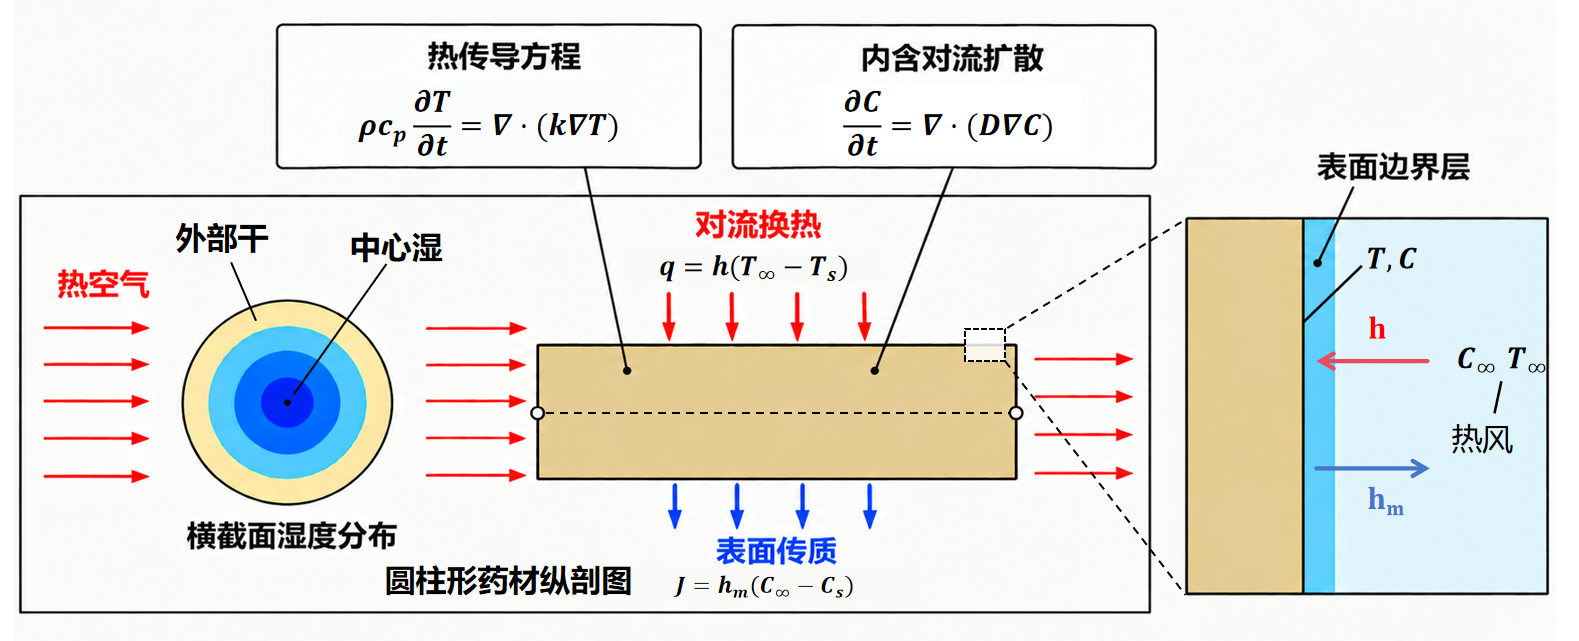
\includegraphics[width=1\linewidth]{pic/illustration.png}
    \caption{圆柱形药材热风烘干的传热传质机理示意图}
    \label{fig:illustration}
\end{figure}


药材初始状态为
\begin{equation}
T(r,0) = T_0 = 28^\circ\text{C}, \qquad C(r,0) = C_0 = 2.55\,\text{kg/kg}.
\end{equation}

\subsection{基本假设}

\begin{itemize}
    \item 药材内部初始温度和含水率在径向上均匀分布；
    \item 忽略轴向和圆周方向的传递，仅考虑半径方向的变化；
    \item 长度在径向控制方程中约去，守恒量按单位轴向长度计算；
    \item 问题一中的 \(\rho, c_p, k\) 为常数，\(D\) 仅依赖 \(C\)；问题二和问题三使用附录 3 的变物性关系；问题四使用附录 4 关系并进一步考虑半径变化。
\end{itemize}

\subsection{统一的热质传递方程}

\subsubsection{热量守恒方程}

取药材内部一微元控制体，由能量守恒定律可知：单位时间内控制体内热量的累积等于净流入控制体的热量与内热源生成热量之和。本文忽略内热源，则单位体积内热量的累积率可表示为
\begin{equation}
Q_v = \rho c_p \frac{\partial T}{\partial t}
\end{equation}
式中，\(Q_v\) 为单位体积热量累积率，\(\rho\) 为药材密度，\(c_p\) 为药材比热容，\(T\) 为药材内部温度，\(t\) 为时间。

药材内部热量主要以导热方式传递。根据傅里叶定律，热流密度与温度梯度成正比、方向相反，即
\begin{equation}
q = -k \nabla T
\end{equation}
式中，\(q\) 为热流密度矢量，\(k\) 为药材热传导系数，\(\nabla\) 表示梯度算子，\(\nabla \cdot\) 表示散度算子。

由能量守恒定律，控制体内热量的累积率等于热流密度的散度，即
\begin{equation}
\rho c_p \frac{\partial T}{\partial t} = -\nabla \cdot q
\end{equation}
将式(2)代入式(3)，得到药材内部温度场的控制方程
\begin{equation}
\rho c_p \frac{\partial T}{\partial t} = \nabla \cdot (k \nabla T)
\end{equation}

\subsubsection{水分扩散方程}

药材内部水分的迁移以扩散为主。根据有效 Fick 定律，水分扩散通量与水分浓度梯度成正比、方向相反，即
\begin{equation}
J_c = -D \nabla C
\end{equation}
式中，\(J_c\) 为水分扩散通量矢量，\(D\) 为水分浓度扩散系数，\(C\) 为药材水分浓度。

由水分质量守恒定律，控制体内水分浓度的变化率等于水分扩散通量的散度，即
\begin{equation}
\frac{\partial C}{\partial t} = -\nabla \cdot J_c
\end{equation}
将式(5)代入式(6)，得到药材内部水分浓度场的控制方程
\begin{equation}
\frac{\partial C}{\partial t} = \nabla \cdot (D \nabla C)
\end{equation}

需要指出的是，题目附录中给出的扩散系数 \(D\) 并非常数，而是与水分浓度 \(C\) 及温度 \(T\) 相关的函数。因此，式(7)应进一步写为
\begin{equation}
\frac{\partial C}{\partial t} = \nabla \cdot \bigl( D(C,T) \, \nabla C \bigr)
\end{equation}

\subsubsection{一维径向模型}

考虑到药材初始温度与含水率分布均匀，且药材几何形状为圆柱体，可作如下简化：忽略沿轴向的变化，忽略沿圆周方向的变化，仅考虑从药材中心到表面的径向变化。由此，三维问题可退化为沿半径方向的一维问题。

在柱坐标系下，对任一标量场 \(u\) 和传输系数 \(q\)，有恒等式
\begin{equation}
\nabla \cdot (q \nabla u) = \frac{1}{r} \frac{\partial}{\partial r} \left( r q \frac{\partial u}{\partial r} \right)
\end{equation}
式中，\(r\) 为到药材中心的径向距离。

将式(9)分别代入温度控制方程(4)和水分浓度控制方程(8)，可得一维径向模型下的控制方程组：
\begin{equation}
\rho(C) c_p(C) \frac{\partial T}{\partial t} = \frac{1}{r} \frac{\partial}{\partial r} \left( r k \frac{\partial T}{\partial r} \right)
\end{equation}
\begin{equation}
\frac{\partial C}{\partial t} = \frac{1}{r} \frac{\partial}{\partial r} \left( r D(C,T) \frac{\partial C}{\partial r} \right)
\end{equation}

\subsection{初始条件与边界条件}

\subsubsection{初始条件}

烘干开始时，药材内部温度和水分浓度分布均匀，由题意可得
\begin{equation}
T(r,0) = 28^\circ\text{C}, \qquad C(r,0) = 2.55\,\text{kg/kg}, \qquad 0 \le r \le R
\end{equation}
式中，\(R\) 为药材半径。根据题目给定尺寸，半径 \(R = 0.02\,\text{m}\)。

\subsubsection{中心对称条件}

在圆柱中心 \(r=0\) 处，由对称性可知热流密度与水分通量均为零，即
\begin{equation}
\left. \frac{\partial T}{\partial r} \right|_{r=0} = 0, \qquad \left. \frac{\partial C}{\partial r} \right|_{r=0} = 0
\end{equation}

\subsubsection{表面对流换热条件}

烘房空气通过对流将热量传递给药材，药材表面温度不一定等于空气温度，药材内部导热与外部对流共同决定其升温过程。由于题目未直接指定药材表面温度，采用 Newton 对流边界条件：
\begin{equation}
-k \left. \frac{\partial T}{\partial r} \right|_{r=R} = h \left[ T(R,t) - T_\infty(t) \right]
\end{equation}
式中，\(h\) 为对流换热系数，\(T_f(t)\) 为烘房温度，其随时间的变化由附件1给出。

\subsubsection{表面对流传质条件}

药材表面含水率与空气水分浓度之间存在差异，水分先从药材内部扩散至表面，再通过气膜传递至空气中。因此，药材表面满足对流传质边界条件
\begin{equation}
-D \left. \frac{\partial C}{\partial r} \right|_{r=R} = h_m \left[ C(R,t) - C_\infty(t) \right]
\end{equation}
式中，\(h_m\) 为对流传质系数，\(C_\infty(t)\) 为烘房空气水分浓度，其随时间的变化由附件1给出。


\subsection{环境数据处理与两阶段约定}

根据给出的离散时刻的烘房温度和空气水分浓度。问题一先用 PCHIP（分段三次 Hermite 保形插值）将原始数据插值到 1s 网格，输出相应结果。问题二至问题四调用边界时采用离散数据的分段线性插值；当查询时间超过数据末端时，取末尾 1000 个数据点的均值作常值延拓。

\subsection{稳定性判断与边界切换}

由附件 1 的稳定性判断得到约 5439s 的稳定起点。为了使阶段初值、边界切换和输出时间原点统一，程序取
\begin{equation}
t_s = 5500\,\text{s}.
\end{equation}

因此，所有全过程计算均按
\begin{equation}
B(t) = 
\begin{cases}
(T_1(t), C_1(t)), & 0 \le t \le t_s, \\
(T_2(t), C_2(t)), & t > t_s,
\end{cases}
\end{equation}
调用边界。其中第一段为附件 1 的变化边界，第二段为稳定阶段边界。问题二的结果表以 \(t_s\) 为新的时间原点，表中 0~10800s 表示绝对时间 5500~16300s；问题三和问题四从原始 \(t = 0\) 开始计时。

\subsection{数值保护约定}

程序在每一步求解后检查数组是否有限，并对经验公式的输入作物理范围保护：问题二、三中评价 \(D(C,T)\) 时将 \(C\) 限制在 \([0.05, 10]\)，\(T_K\) 限制在 \([273.15, 373.15]\,\text{K}\)，并将 \(D\) 限制在 \([10^{-14}, 10^{-3}]\,\text{m}^2/\text{s}\)；问题四采用同样的温度和扩散系数保护。状态量的保护范围为 \(-50 \le T \le 250^\circ\text{C}\)，\(0 \le C \le 10\)。验证结果表明正式计算未触及这些保护边界，因此我们进行的保护操作不改变本题数值解。


\section{问题一：常物性径向模型的建立和求解}
\subsection{模型建立与求解}

本文建立的一维径向传热传质控制方程属于非线性偏微分方程组，难以获得解析解。为此，本文采用显式有限差分法（FDM）对空间域和时间域进行离散，通过时间推进循环求解药材内部温度和水分浓度的时空分布。

\subsubsection{时空离散与网格划分}

在空间域上，将药材半径 \(R\) 离散为 \(N_r = 21\) 个节点，空间步长 \(\Delta r = 0.001\,\text{m}\)，节点位置为 \(r_i = i\Delta r\)（\(i = 0,1,\dots,N_r-1\)）。在时间域上，取时间步长 \(\Delta t = 1\,\text{s}\)，记 \(t_n = n\Delta t\)（\(n = 0,1,\dots,N_t-1\)），本文问题一的总计算区间为 \(0 \le t_n \le 1800\,\text{s}\)。

令系数
\begin{equation}
\alpha = \frac{k}{\rho c_p}, \qquad \lambda_i^+ = 1 + \frac{\Delta r}{2r_i}, \qquad \lambda_i^- = 1 - \frac{\Delta r}{2r_i}.
\end{equation}

\subsubsection{边界条件的数据预处理}

在算法的时间推进过程中，表面节点及内部节点的更新均高度依赖于烘房环境的实时边界值 \(T_\infty(t)\) 和 \(C_\infty(t)\)。由于仅提供了有限个离散时间点的环境参数数据，必须通过插值获取任意时间步 \(n+1\) 对应的环境值 \(T_\infty^{n+1}\) 和 \(C_\infty^{n+1}\)。

由于显式有限差分法对边界条件的一阶导数十分敏感，若采用常规线性插值，其在节点处导数不连续（折点）的非光滑特性极易引起数值震荡，进而导致求解发散。因此，本文选取 PCHIP（分段三次 Hermite 插值多项式）对烘房环境参数进行插值。PCHIP 不仅保证了插值曲线的一阶导数连续，符合物理量平滑变化的规律，同时\textbf{保持数据的单调性，避免非物理的过冲现象}。这使得插值得到的水分浓度不会出现负值，为后续偏微分方程的数值求解提供了平滑且稳定的边界输入，保障了计算收敛性。

\subsubsection{内部节点更新}

对内部节点 \(i = 1,2,\dots,N_r-2\)，温度采用显式柱坐标中心差分格式：
\begin{equation}
T_i^{n+1} = T_i^n + \alpha \frac{\Delta t}{\Delta r^2} \left[ \lambda_i^+ T_{i+1}^n - 2T_i^n + \lambda_i^- T_{i-1}^n \right].
\end{equation}

水分方程则采用\textbf{守恒型界面通量离散}，而不再直接使用节点扩散系数。定义界面扩散系数为左右节点浓度的算术平均：
\begin{equation}
D_{i+1/2}^n = D\left( \frac{C_i^n + C_{i+1}^n}{2} \right), \qquad D_{i-1/2}^n = D\left( \frac{C_{i-1}^n + C_i^n}{2} \right).
\end{equation}
则内部节点的水分更新式为
\begin{equation}
\begin{aligned}
C_i^{n+1} = C_i^n &+ \frac{\Delta t}{\Delta r^2} \Big[ \lambda_i^+ D_{i+1/2}^n (C_{i+1}^n - C_i^n) \\
&+ \lambda_i^- D_{i-1/2}^n (C_{i-1}^n - C_i^n) \Big].
\end{aligned}
\end{equation}
同一界面系数由相邻两个控制体共用，因此内部界面通量在全局求和时成对抵消，从而在数值上保证质量守恒。

\subsubsection{中心节点更新}

在圆柱中心 \(r=0\) 处，由对称性可知热流与水分通量均为零。利用洛必达法则对柱坐标方程取中心极限，得到中心节点的更新公式：
\begin{equation}
T_0^{n+1} = T_0^n + 4\alpha \frac{\Delta t}{\Delta r^2} (T_1^n - T_0^n),
\end{equation}
\begin{equation}
C_0^{n+1} = C_0^n + 4D_{1/2}^n \frac{\Delta t}{\Delta r^2} (C_1^n - C_0^n),
\end{equation}
其中 \(D_{1/2}^n = D\left((C_0^n + C_1^n)/2\right)\)。

\subsubsection{表面节点更新}

记 \(i_s = N_r-1\)，表面节点控制体的单位长度体积为
\begin{equation}
V_s = \pi \left[ R_0^2 - \left( R_0 - \frac{\Delta r}{2} \right)^2 \right] = \pi \Delta r^2 \left( i_s - \frac{1}{4} \right).
\end{equation}

温度表面更新式由内表面导热、外表面对流以及控制体热量累积三部分构成：
\begin{equation}
\begin{aligned}
T_{i_s}^{n+1} = T_{i_s}^n &+ \Delta t \Bigg[ \frac{2(i_s - \frac{1}{2})k}{\rho c_p (i_s - \frac{1}{4})\Delta r^2} (T_{i_s-1}^n - T_{i_s}^n) \\
&+ \frac{2 i_s h}{\rho c_p (i_s - \frac{1}{4})\Delta r} (T_\infty^{n+1} - T_{i_s}^n) \Bigg].
\end{aligned}
\end{equation}

令表面处界面扩散系数为 \(D_{s-1/2}^n = D\left( \frac{C_{i_s-1}^n + C_{i_s}^n}{2} \right)\)，水分表面更新式为
\begin{equation}
\begin{aligned}
C_{i_s}^{n+1} = C_{i_s}^n &+ \Delta t \Bigg[ \frac{2(i_s - \frac{1}{2}) D_{s-1/2}^n}{(i_s - \frac{1}{4})\Delta r^2} (C_{i_s-1}^n - C_{i_s}^n) \\
&+ \frac{2 i_s h_m}{(i_s - \frac{1}{4})\Delta r} (C_\infty^{n+1} - C_{i_s}^n) \Bigg].
\end{aligned}
\end{equation}
式中，\(h\) 和 \(h_m\) 分别为对流换热系数和对流传质系数。此处环境边界值 \(T_\infty^{n+1}\) 和 \(C_\infty^{n+1}\) 使用下一时刻的插值取值，而表面状态依赖当前时刻值，这正是本文程序显式实现中的边界处理方式。

\subsubsection{求解流程与结果输出}

上述显式差分的求解流程如图 \ref{fig:algorithm1} 所示。算法首先初始化温度与水分浓度矩阵，并计算热扩散系数；随后进入时间推进循环（\(n = 0\) 到 \(N_t-2\)），在每一时间步内，先利用 PCHIP 插值获取下一时刻的环境值 \(T_\infty^{n+1}\) 和 \(C_\infty^{n+1}\)，接着计算当前时刻各节点的界面扩散系数 \(D_{i+1/2}^n\)，并依次更新内部节点、中心节点及表面节点的温度与水分浓度；循环结束后，输出完整的温度矩阵 \(T_i^n\) 和水分矩阵 \(C_i^n\)，并按要求提取特定时刻与径向位置的切片数据。

\subsubsection{稳定性条件}

显式差分格式需满足 CFL 稳定性条件。在本题参数下，
\begin{equation}
\frac{\alpha \Delta t}{\Delta r^2} = 0.1689, \qquad 4 \frac{\alpha \Delta t}{\Delta r^2} = 0.6754 < 1.
\end{equation}
初始含水率下中心水分更新系数约为 \(0.0198\)，满足显式推进的稳定性要求。程序输出 \(0\sim1800\,\text{s}\) 内每隔 \(1\,\text{s}\)、径向每隔 \(0.1\,\text{cm}\) 的完整温度和水分结果。论文用表在 \(t \in \{100,300,600,900,1200,1500,1800\}\,\text{s}\) 以及 \(r \in \{0,0.5,1,1.5,2\}\,\text{cm}\) 处提取。

\begin{figure}[H]
    \centering
    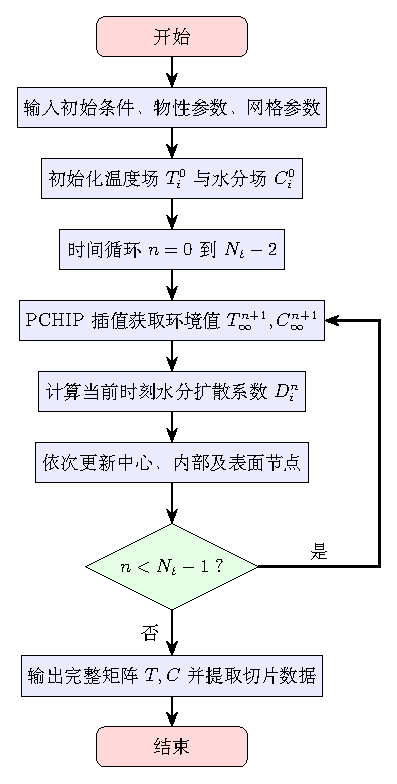
\includegraphics[width=0.5\linewidth]{pic/algorithm1.pdf}
    \caption{问题一算法流程图}
    \label{fig:algorithm1}
\end{figure}

\subsubsection{求解结果}

\begin{table}[htbp]
    \centering
    \caption{30分钟内药材的温度}
    \label{tab:temp}
    \renewcommand{\arraystretch}{1.5} % 调整行高，使其更像图片中的比例
    \setlength{\tabcolsep}{10pt} % 增大列间距，使表格适当变宽
    \begin{tabular}{|c|c|c|c|c|c|}
        \hline
        \multirow{2}{*}{时间/s} & \multicolumn{5}{c|}{到药材中心的距离/cm} \\
        \cline{2-6}
         & 0 & 0.5 & 1 & 1.5 & 2 \\
        \hline
        100 & 28.0000 & 28.0003 & 28.0039 & 28.032 & 28.1803 \\
        \hline
        300 & 28.0408 & 28.0636 & 28.1517 & 28.3681 & 28.8504 \\
        \hline
        600 & 28.4543 & 28.5372 & 28.8053 & 29.3175 & 30.1667 \\
        \hline
        900 & 29.3262 & 29.4604 & 29.8781 & 30.6192 & 31.7329 \\
        \hline
        1200 & 30.5456 & 30.7128 & 31.2256 & 32.1166 & 33.4336 \\
        \hline
        1500 & 31.9994 & 32.1906 & 32.7705 & 33.7517 & 35.1255 \\
        \hline
        1800 & 33.5798 & 33.7764 & 34.3684 & 35.3666 & 36.7905 \\
        \hline
    \end{tabular}
\end{table}


\begin{table}[htbp]
    \centering
    % 表格标题，加粗，字号稍大
    \textbf{\large 表 2\quad 30 分钟内药材的水分浓度}
    \vspace{5mm} % 标题与表格的间距
    
    % 增加行高，使表格更美观，与原图一致
    \renewcommand{\arraystretch}{1.6}
    \setlength{\tabcolsep}{10pt} % 增大列间距，使表格适当变宽    
    % 定义表格列：共6列，全部居中，且有竖线边框
    \begin{tabular}{|c|c|c|c|c|c|}
        \hline
        % 第一行：合并前两行的“时间/s”，合并后五列的“到药材中心距离/cm”
        \multirow{2}{*}{时间/s} & \multicolumn{5}{c|}{到药材中心距离/cm} \\
        \cline{2-6} % 在第2到第6列画横线
        % 第二行：空出第一列，填写距离表头
         & 0 & 0.5 & 1 & 1.5 & 2 \\
        \hline
        % 数据部分
        100 & 2.55 & 2.55 & 2.55 & 2.55 & 2.2875 \\
        \hline
        300 & 2.55 & 2.55 & 2.55 & 2.5486 & 2.066 \\
        \hline
        600 & 2.55 & 2.55 & 2.55 & 2.5342 & 1.8847 \\
        \hline
        900 & 2.55 & 2.55 & 2.5495 & 2.5041 & 1.7598 \\
        \hline
        1200 & 2.55 & 2.55 & 2.5478 & 2.4647 & 1.6623 \\
        \hline
        1500 & 2.55 & 2.5499 & 2.544 & 2.4211 & 1.5816 \\
        \hline
        1800 & 2.55 & 2.5496 & 2.5376 & 2.3762 & 1.5125 \\
        \hline
    \end{tabular}
\end{table}

\begin{figure}
    \centering
    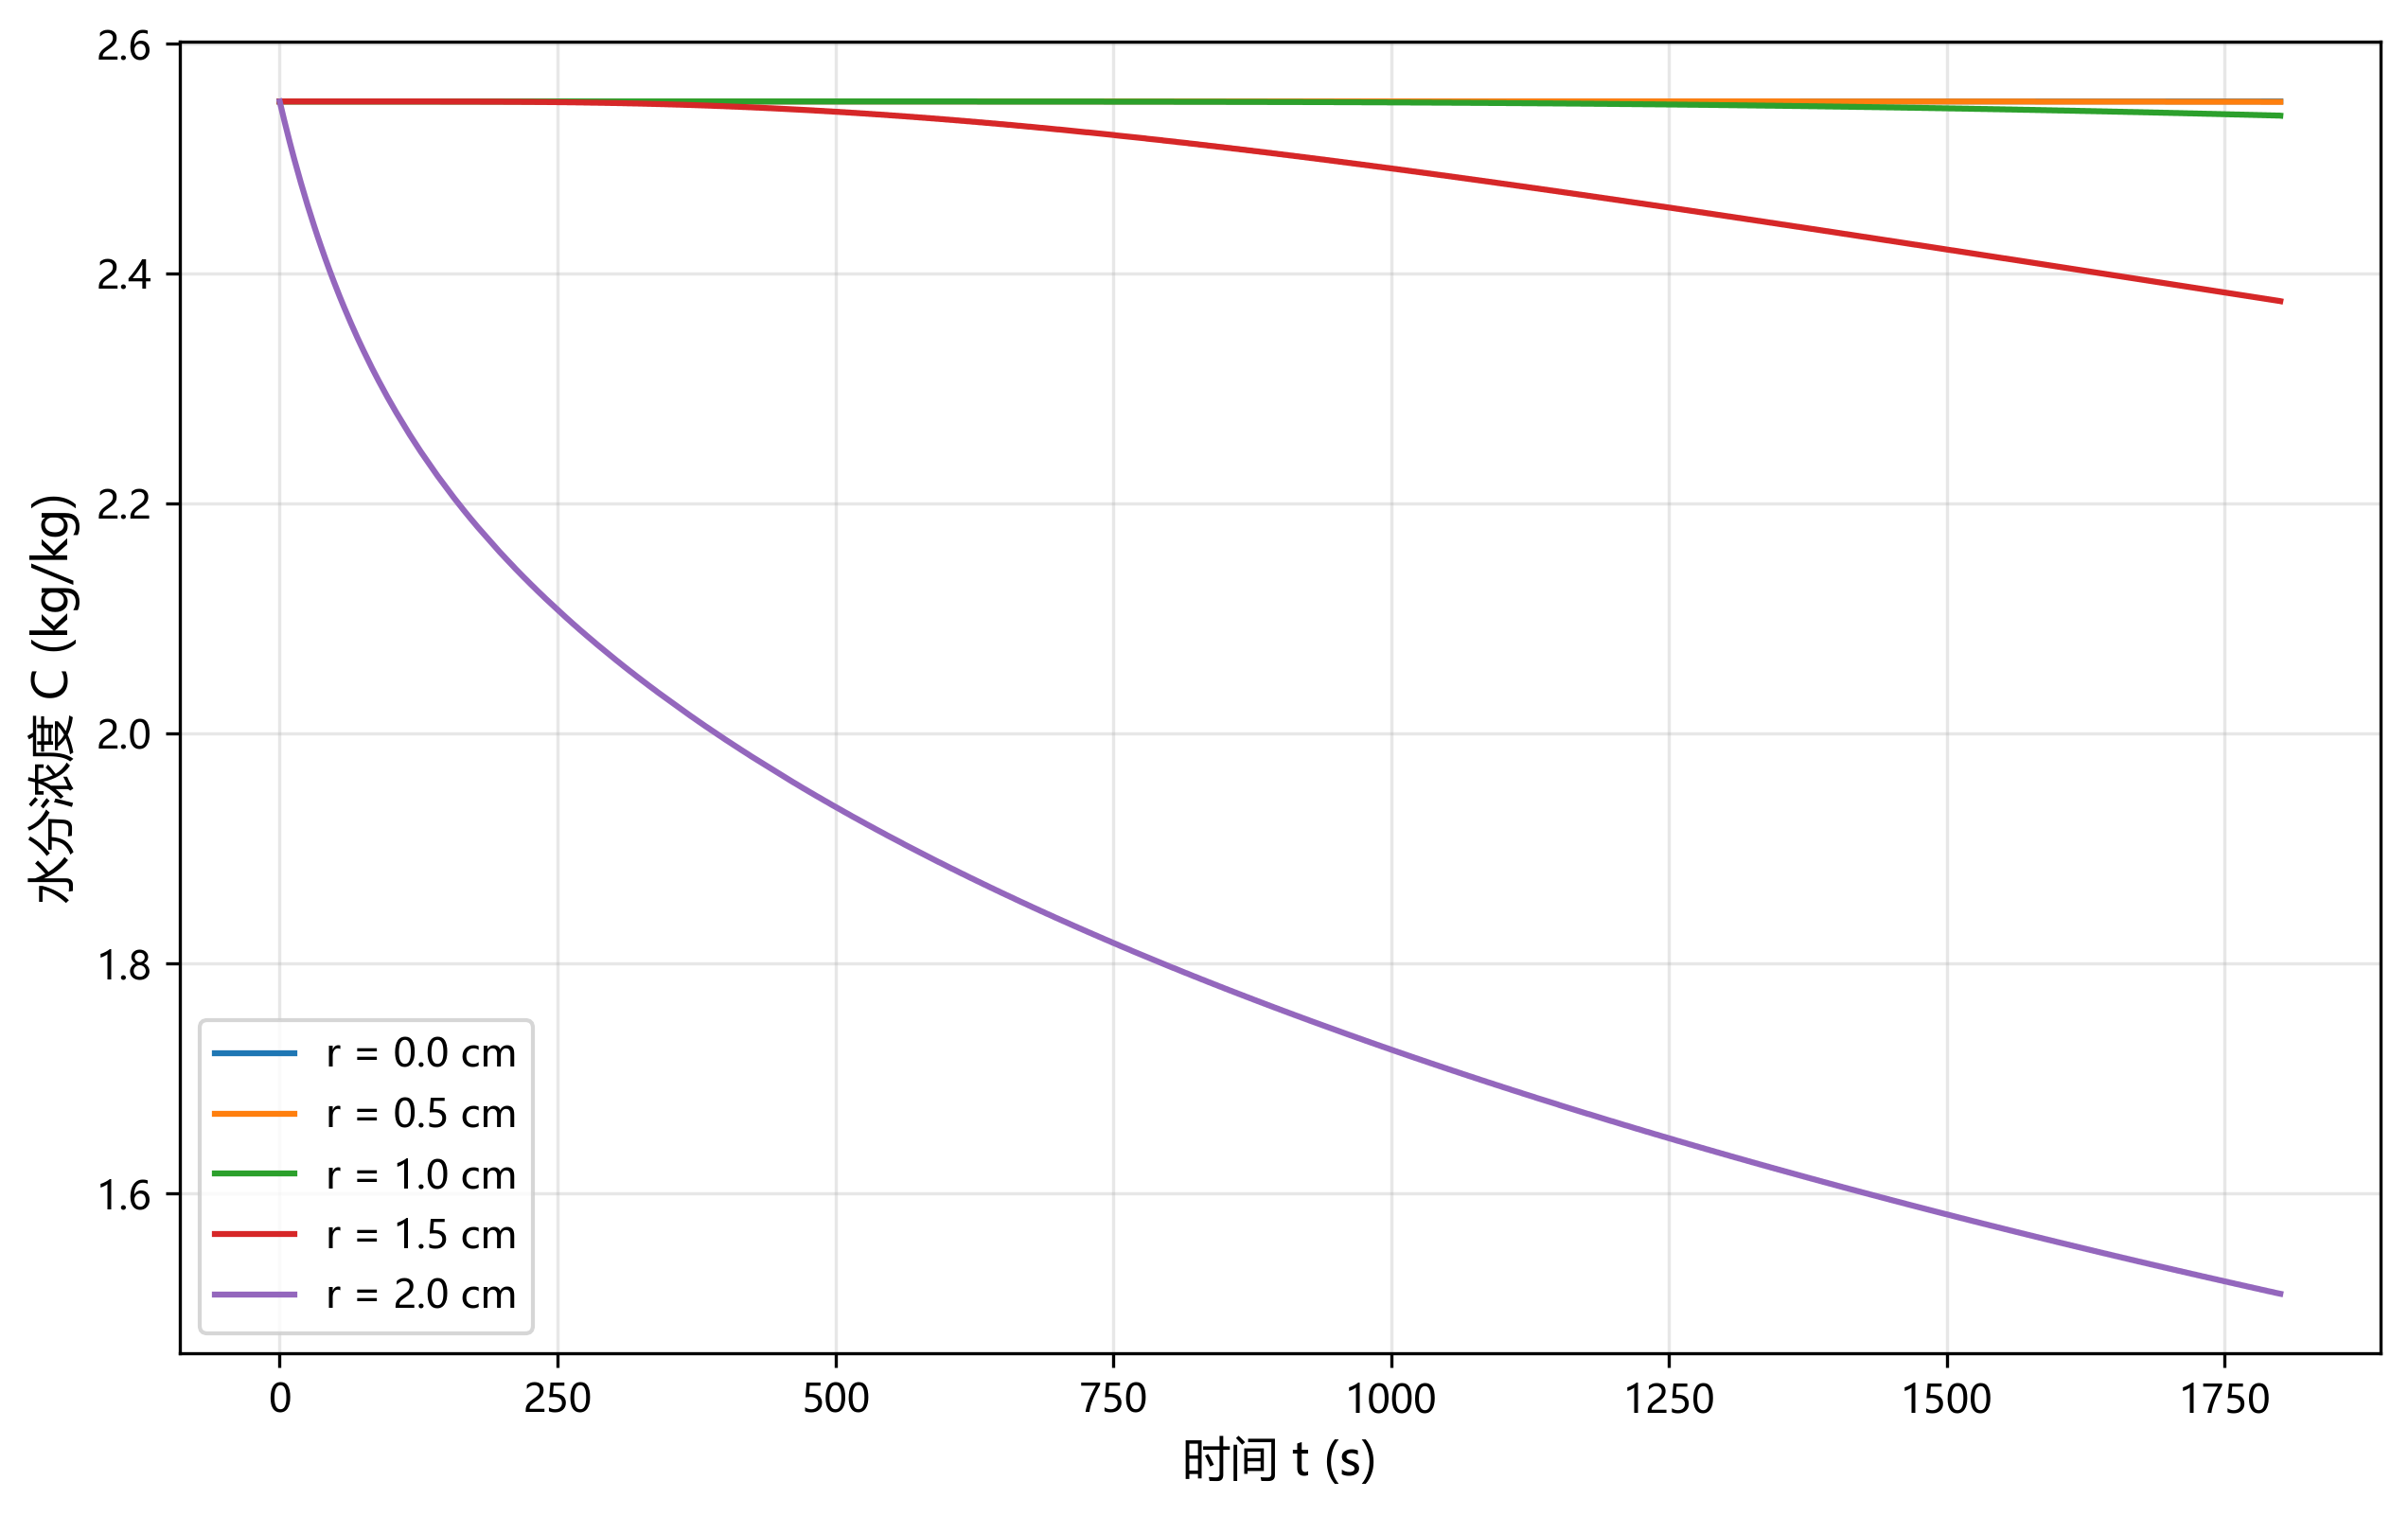
\includegraphics[width=1\linewidth]{pic/q1_1_水分时间演化图.png}
    \caption{问题一水分浓度随时间的变化}
    \label{fig:q1_moisture_time}
\end{figure}

\begin{figure}
    \centering
    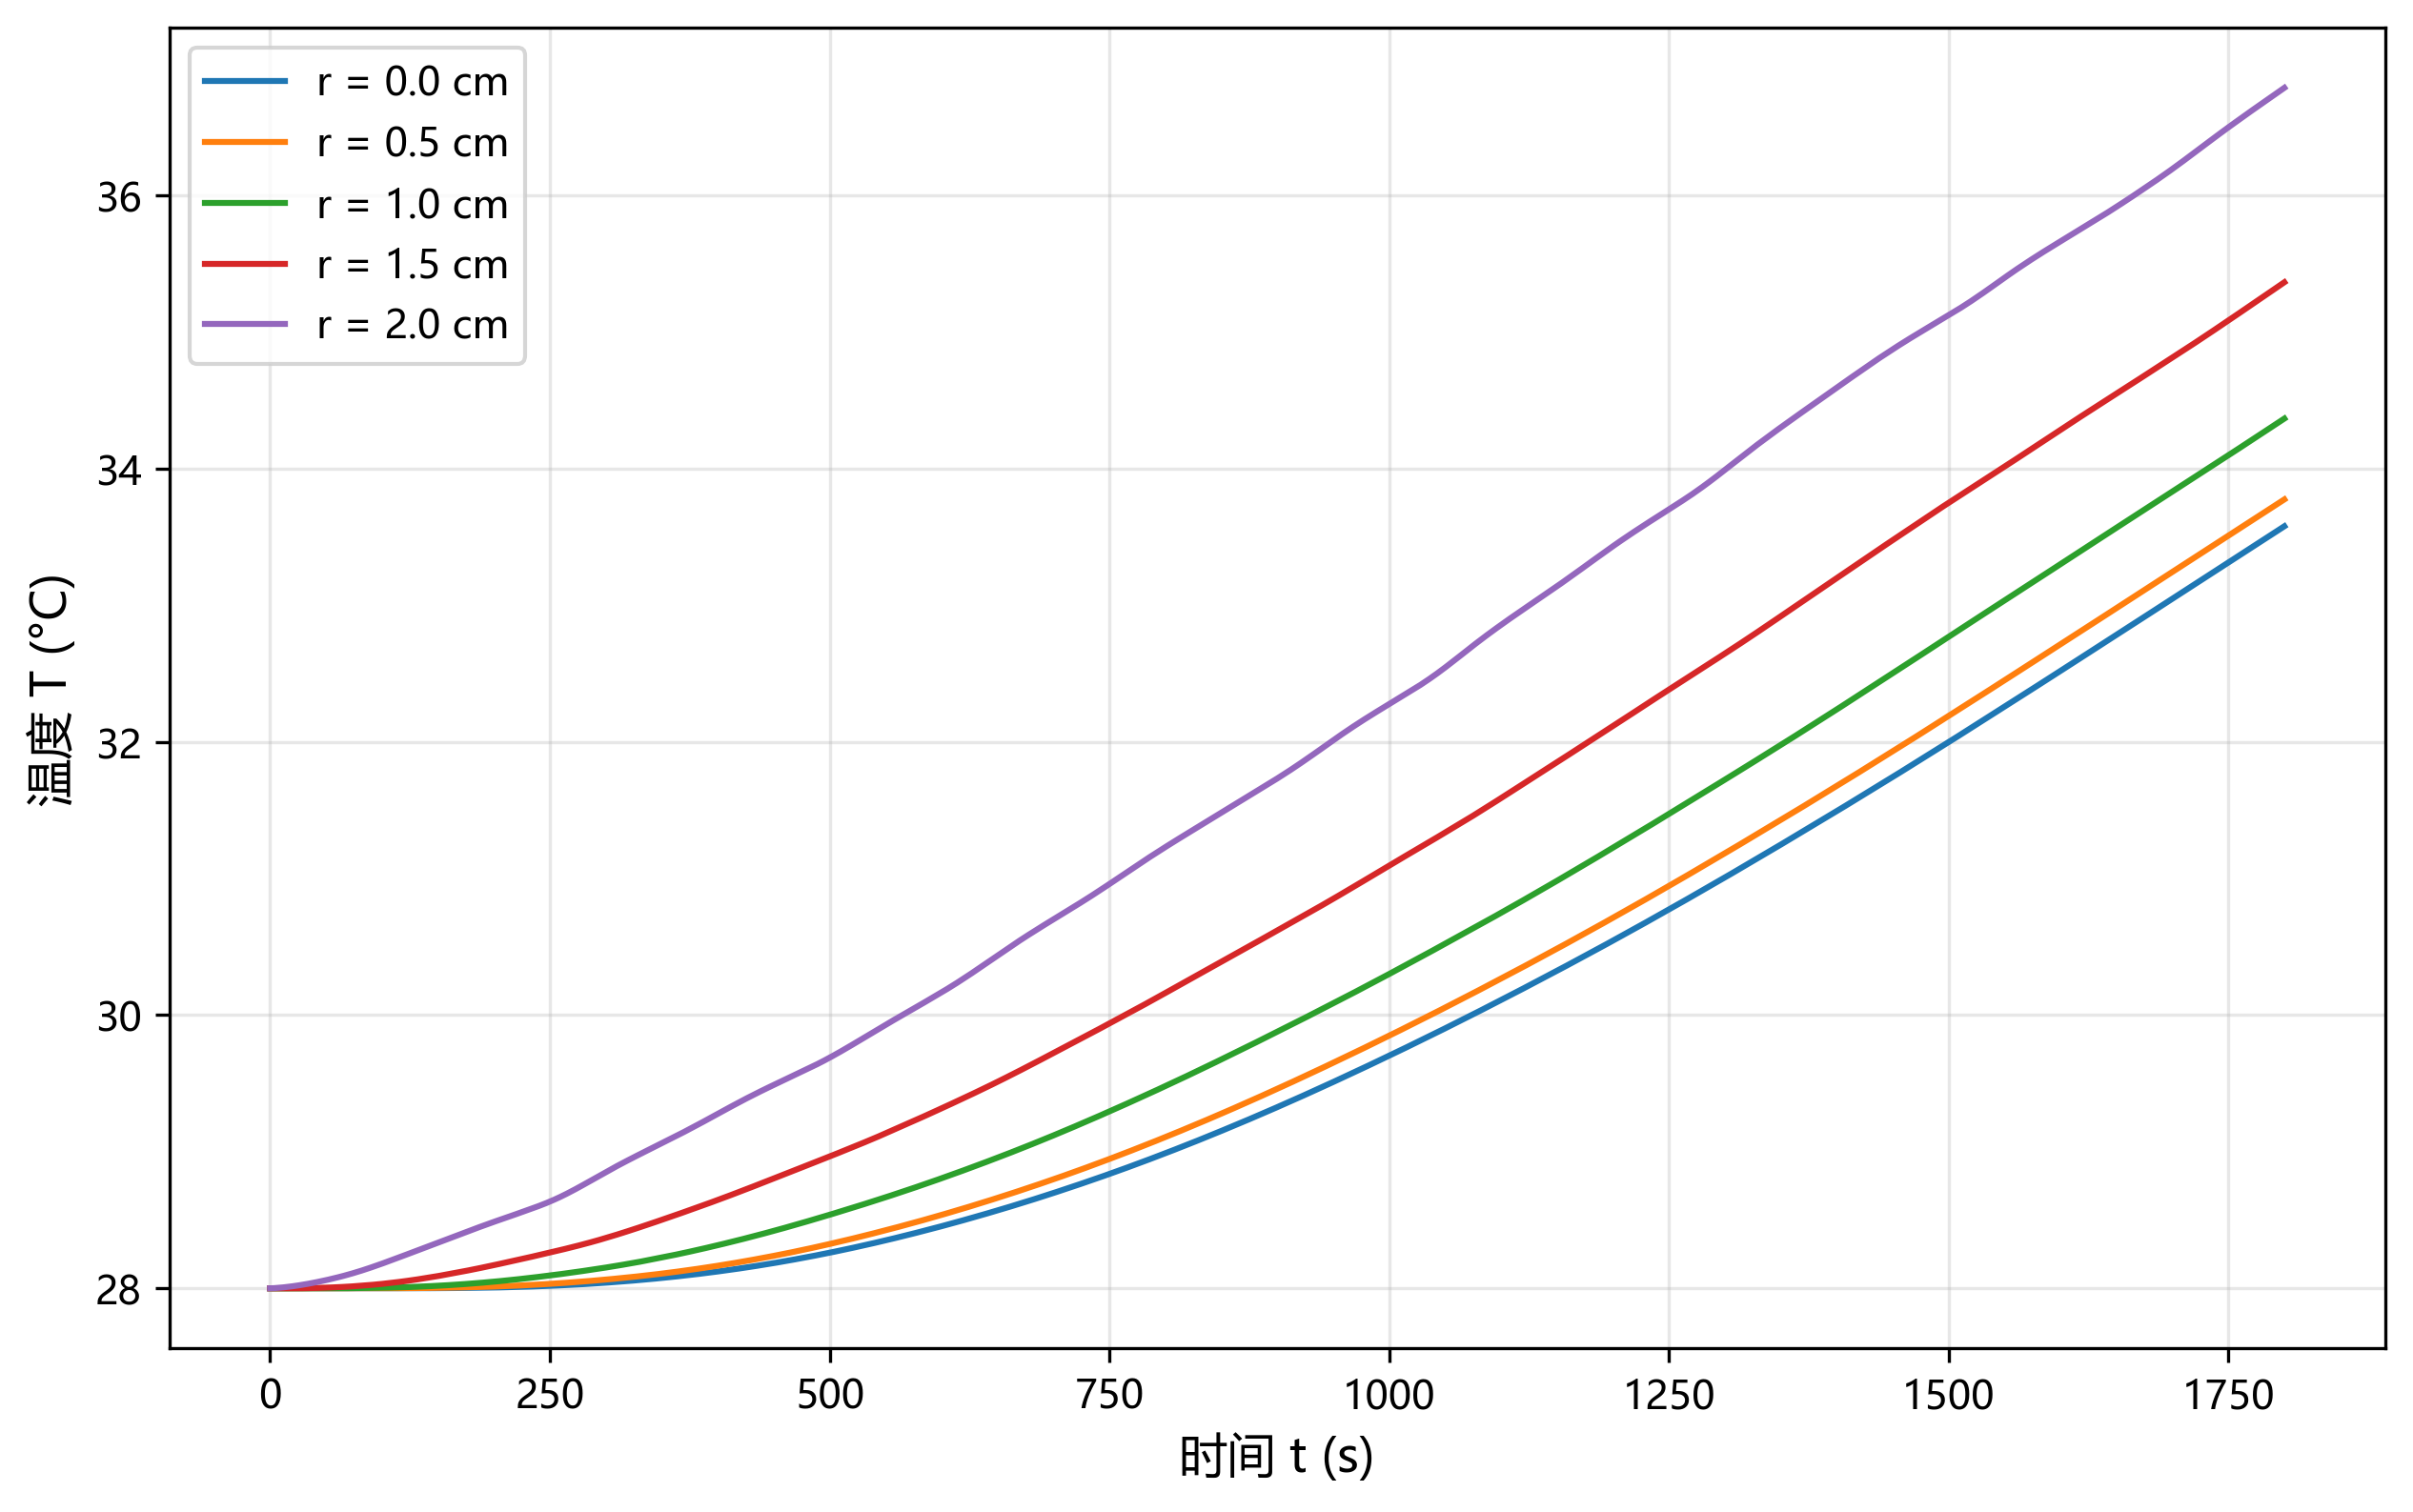
\includegraphics[width=1\linewidth]{pic/q1_2_温度时间演化图.png}
    \caption{问题一温度随时间的变化}
    \label{fig:q1_temperature_time}
\end{figure}

\begin{figure}
    \centering
    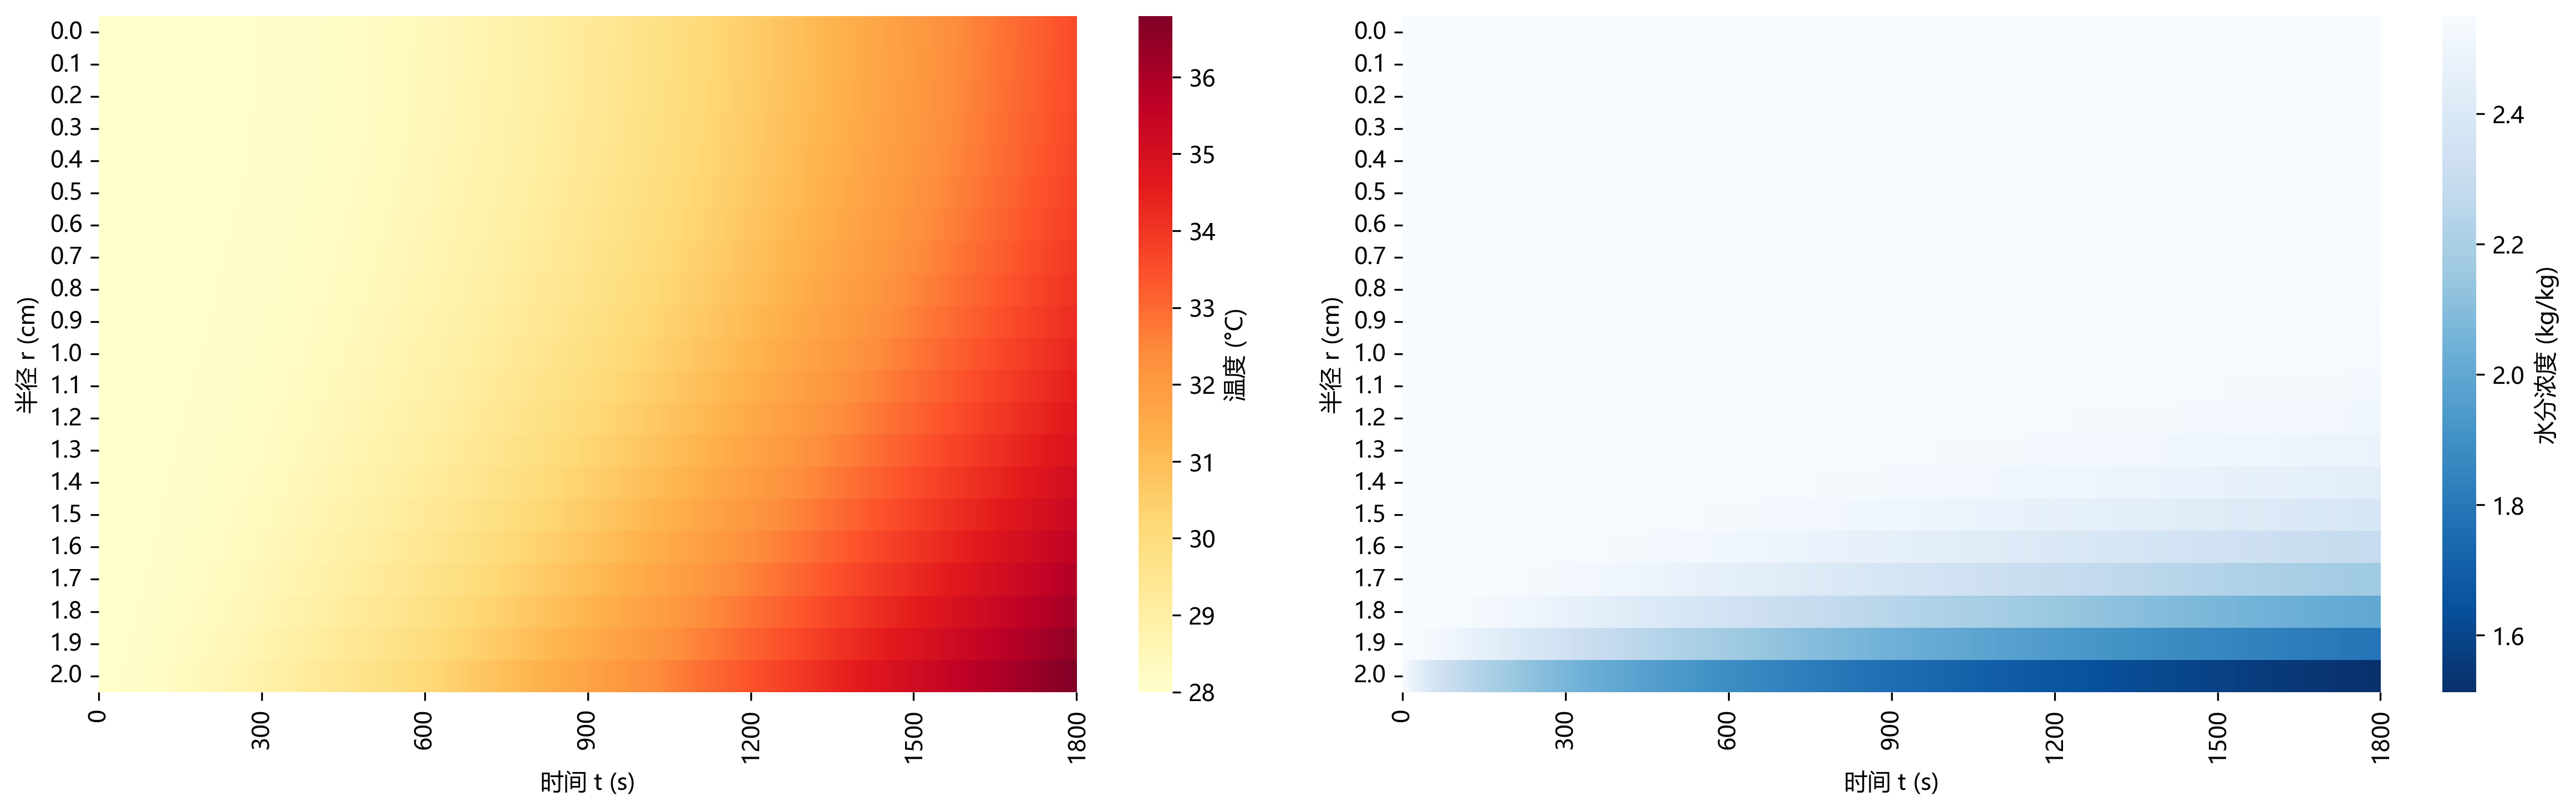
\includegraphics[width=1\linewidth]{pic/q1_3_温度和水分热力图.png}
    \caption{问题一温度和水分浓度热力图}
    \label{fig:q1_heatmap}
\end{figure}

\begin{figure}
    \centering
    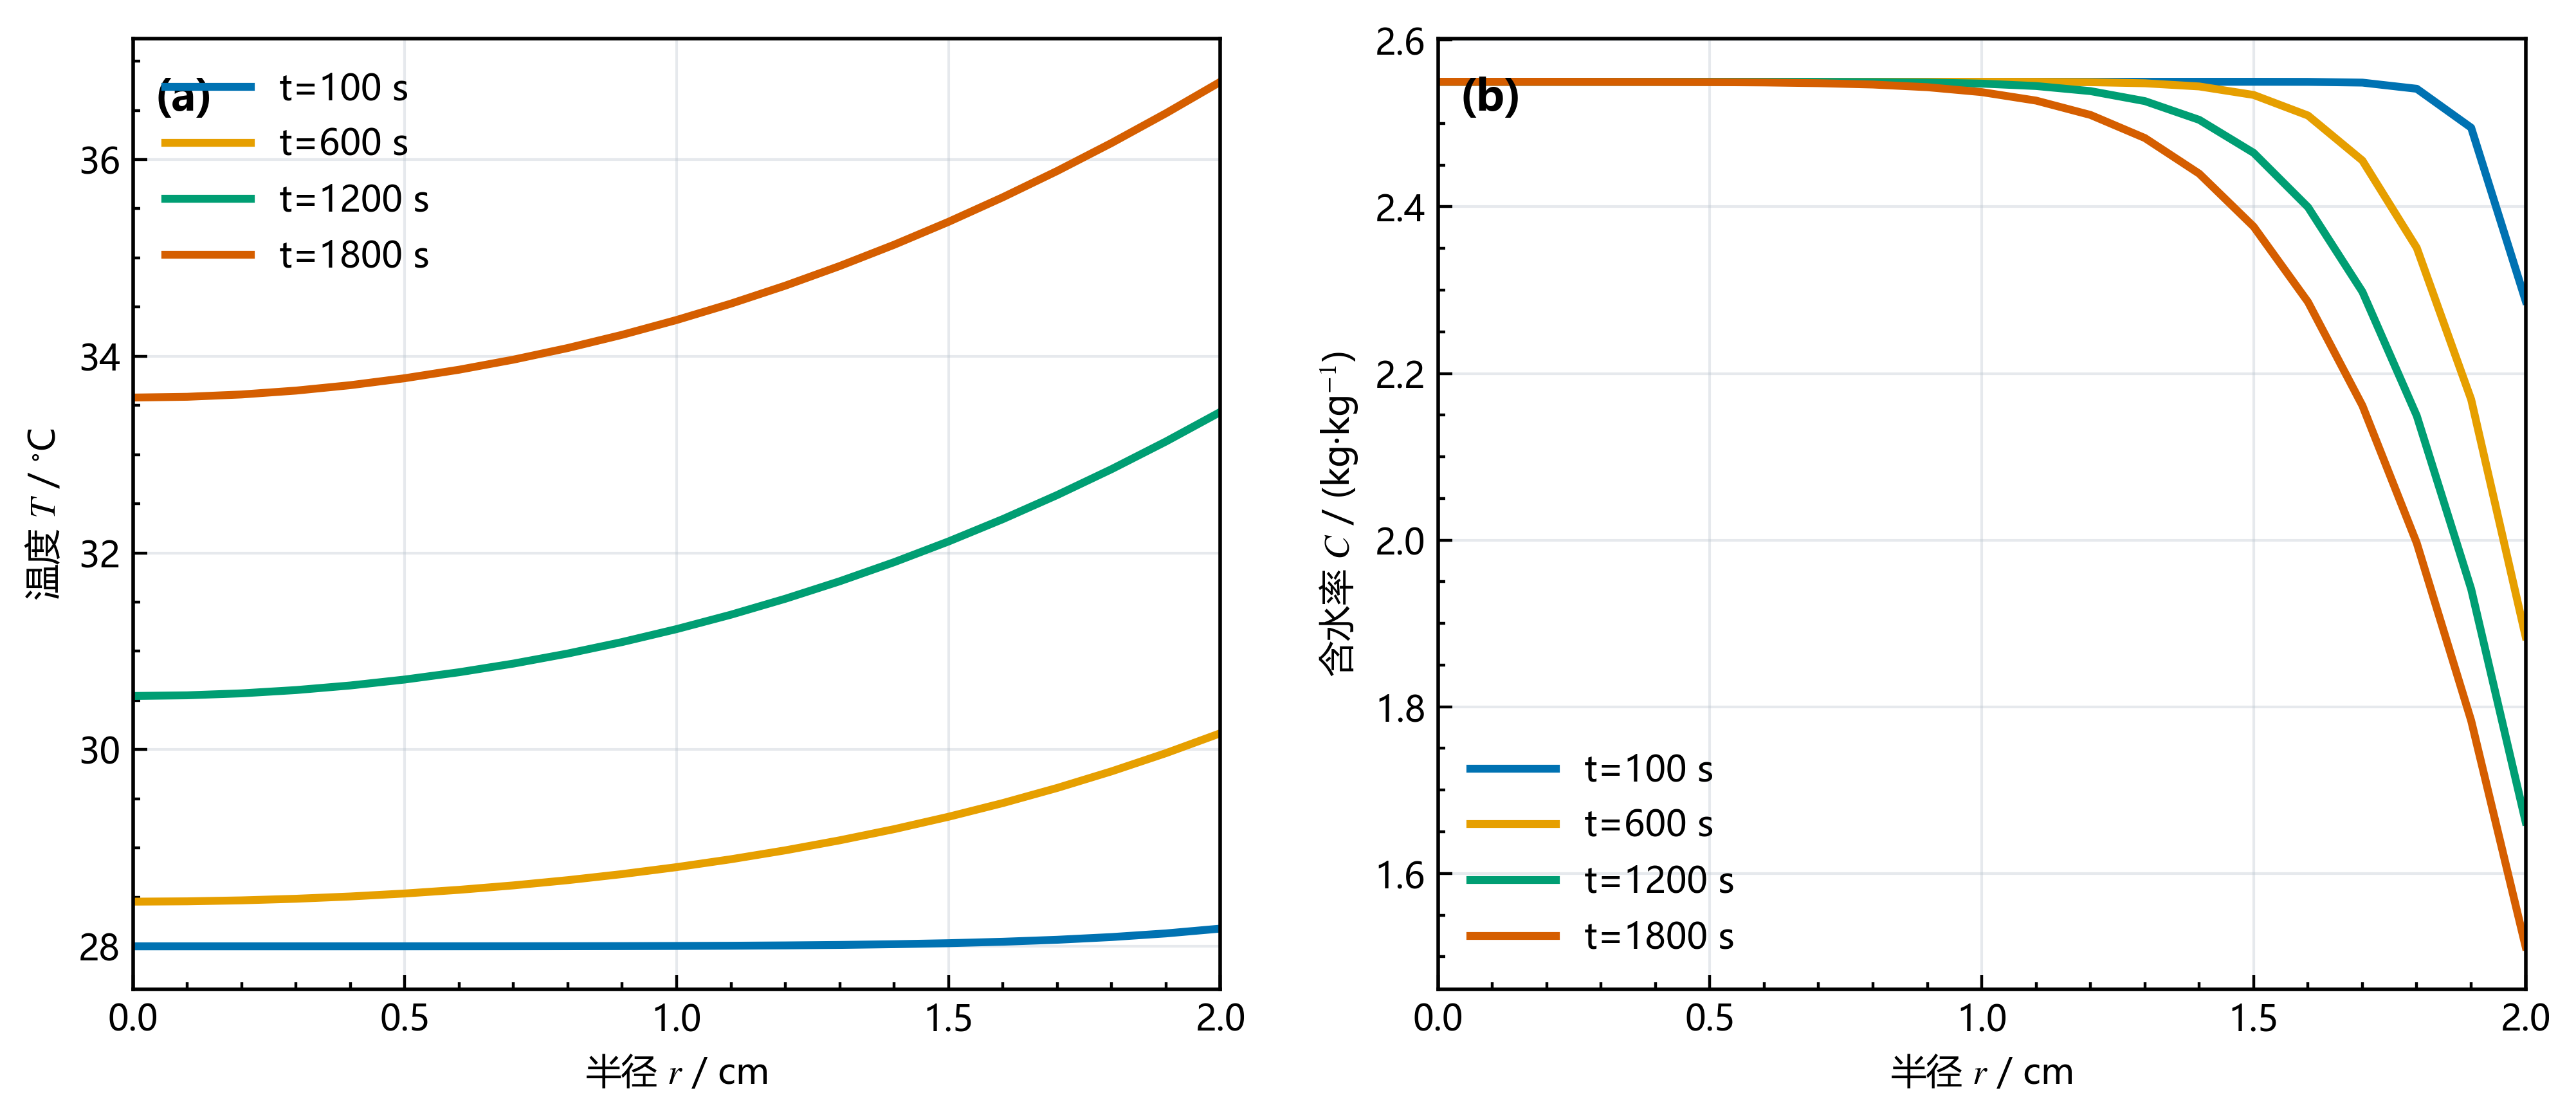
\includegraphics[width=1\linewidth]{pic/q1_4_问题一径向温度和含水率分布.png}
    \caption{问题一径向温度和含水率分布}
    \label{fig:q1_radial}
\end{figure}

结果表明，总能量变化曲线与边界热流累积曲线在整个模拟时段内几乎完全重合；总水分变化曲线与边界质流累积曲线同样几乎完全重合。两项守恒误差均远小于 5\% 的工程容许阈值，充分证明了本文所建立的显式有限差分算法具有良好的守恒性与数值稳定性，能够为后续中药材烘干过程的温度场与水分场求解提供可靠的数值保障。





















%%%%%%%%%%%%%%%%%%%%%%%%%%%%%%%%%%%%%%%%%%%%%%%%%%%%%%%%%%%%% 
\newpage
\section{问题二：变物性两阶段模型的建立和求解}
\subsection{模型建立}

问题一将密度 \(\rho\)、比热容 \(c_p\)、热传导系数 \(k\) 视为常数，水分扩散系数 \(D\) 仅依赖 \(C\)。然而整个烘干过程持续 \(2\sim3\) 天，药材内部水分浓度发生显著变化，物性参数也随之改变，且烘房环境由预热平衡阶段过渡到恒温干燥阶段。因此，问题二在问题一的基础上，将物性参数改为随局部温度与水分浓度变化的函数，并考虑热质传递的双向耦合效应。

\subsubsection{变物性关系}

问题二使用给出的经验关系：
\begin{equation}
\rho(C) = 650 + 128C,
\end{equation}
\begin{equation}
c_p(C) = 1450 + 2736\frac{C}{C+1},
\end{equation}
\begin{equation}
k(C) = 0.21 + 0.38\frac{C}{C+1},
\end{equation}
\begin{equation}
D(C,T) = 2.4\times 10^{-3}\exp\left(-\frac{0.45}{C}\right)\exp\left(-\frac{3850}{T_K}\right),
\end{equation}
其中 \(T_K = T + 273.15\) 为开尔文温度。

需要强调的是：预热平衡与恒温干燥这两个阶段使用的是同一套附录 3 物性公式，两阶段的差异体现在外部环境边界与时间分段上，而非重新替换物性参数。

\subsubsection{双向耦合关系}

在变物性条件下，温度场与水分浓度场之间形成双向耦合，耦合路径为：
\begin{align*}
    C &\rightarrow \rho, c_p, k \rightarrow T, \\
    (C,T) &\rightarrow D \rightarrow C.
\end{align*}
即水分浓度的变化通过改变密度、比热容与导热系数进而影响温度场；同时温度与水分浓度又共同决定水分扩散系数，进而反过来影响水分浓度场。这与问题一中温度场不依赖水分场的准线性情形形成本质区别。

\subsection{阶段切换与恒温段初值}

整个烘干过程按统一建模框架中的约定划分为两段：预热平衡段与恒温干燥段，切换时刻取 \(t_s = 5500\,\text{s}\)。预热阶段由 \(T = 28^{\circ}\text{C},\ C = 2.55\,\text{kg/kg}\) 的均匀初态开始，使用绝对时间 \(0\sim5500\,\text{s}\) 的附件 1 边界进行求解，得到 \(5500\,\text{s}\) 时刻的温度与水分剖面并保存为输出文件。

恒温段以该剖面为初值，再计算 \(10800\,\text{s}\)，生成问题二的最终结果。因此，恒温段求解器内部的时间记为 \(\tau\)，而边界查询使用绝对时间 \(t = t_s + \tau\)：
\begin{equation}
T_\infty^{n+1} = T_2(t_s + \tau_{n+1}), \qquad C_\infty^{n+1} = C_2(t_s + \tau_{n+1}),
\end{equation}
其中 \(T_2, C_2\) 为统一建模框架中定义的稳定阶段边界函数。结果文件中的时间列为 \(\tau = 0,1,\dots,10800\,\text{s}\)。

\subsection{系数滞后的后向 Euler 半隐式格式}

由于 \(\rho, c_p, k, D\) 均为 \(C\) 与 \(T\) 的函数，直接采用显式格式会受严格的稳定性条件限制。为此，本文采用\textbf{系数滞后的后向 Euler 半隐式格式}：每一时间步内，先由旧时刻的 \(C^n, T^n\) 计算物性参数与界面系数，再对新时刻的未知量组装三对角方程组并求解。该格式兼顾了后向 Euler 的无条件稳定性与显式物性计算的简洁性。

空间网格取 \(r_i = i\Delta r\)，\(\Delta r = 0.001\,\text{m}\)，\(N_r = 21\)；时间步长 \(\Delta t = 1\,\text{s}\)。界面处的物性系数取左右节点算术平均：
\begin{equation}
k_{i+1/2}^n = k\left(\frac{C_i^n + C_{i+1}^n}{2}\right),
\end{equation}
\begin{equation}
D_{i+1/2}^n = D\left(\frac{C_i^n + C_{i+1}^n}{2}, \frac{T_i^n + T_{i+1}^n}{2}\right).
\end{equation}

\subsubsection{内部节点的隐式方程}

对内部节点 \(i = 1,2,\dots,N_r-2\)，定义
\begin{equation}
a_i^T = \frac{\Delta t}{\rho(C_i^n)c_p(C_i^n)\Delta r^2}, \qquad \lambda_i^\pm = 1 \pm \frac{\Delta r}{2r_i},
\end{equation}
则温度三对角方程为
\begin{equation}
\begin{aligned}
&-a_i^T \lambda_i^- k_{i-1/2}^n T_{i-1}^{n+1} + \left[1 + a_i^T\left(\lambda_i^- k_{i-1/2}^n + \lambda_i^+ k_{i+1/2}^n\right)\right]T_i^{n+1} \\
&\quad - a_i^T \lambda_i^+ k_{i+1/2}^n T_{i+1}^{n+1} = T_i^n.
\end{aligned}
\end{equation}

水分内部方程具有相同的守恒结构。令 \(a^C = \Delta t/\Delta r^2\)，则
\begin{equation}
\begin{aligned}
&-a^C \lambda_i^- D_{i-1/2}^n C_{i-1}^{n+1} + \left[1 + a^C\left(\lambda_i^- D_{i-1/2}^n + \lambda_i^+ D_{i+1/2}^n\right)\right]C_i^{n+1} \\
&\quad - a^C \lambda_i^+ D_{i+1/2}^n C_{i+1}^{n+1} = C_i^n.
\end{aligned}
\end{equation}

\subsubsection{中心节点的隐式方程}

令 \(k_{1/2}^n = k\left((C_0^n + C_1^n)/2\right)\)，\(\beta_T = \Delta t/[\rho(C_0^n)c_p(C_0^n)\Delta r^2]\)，则中心温度满足
\begin{equation}
\left(1 + 4\beta_T k_{1/2}^n\right)T_0^{n+1} - 4\beta_T k_{1/2}^n T_1^{n+1} = T_0^n.
\end{equation}

相应地，令
\begin{equation}
D_{1/2}^n = D\left(\frac{C_0^n + C_1^n}{2}, \frac{T_0^n + T_1^n}{2}\right),
\end{equation}
中心水分方程为
\begin{equation}
\left(1 + 4a^C D_{1/2}^n\right)C_0^{n+1} - 4a^C D_{1/2}^n C_1^{n+1} = C_0^n.
\end{equation}

\subsubsection{表面节点的隐式方程}

记 \(i_s = N_r-1\)，\(V_f = i_s - 1/4\)，令
\begin{equation}
k_s^n = k\left(\frac{C_{i_s-1}^n + C_{i_s}^n}{2}\right),
\end{equation}
\begin{equation}
\beta_s^T = \frac{\Delta t}{\rho(C_{i_s}^n)c_p(C_{i_s}^n)V_f \Delta r^2}, \quad A_T = 2\left(i_s - \frac{1}{2}\right)k_s^n, \quad B_T = 2i_s h \Delta r,
\end{equation}
则表面温度方程为
\begin{equation}
-\beta_s^T A_T T_{i_s-1}^{n+1} + \left[1 + \beta_s^T(A_T + B_T)\right]T_{i_s}^{n+1} = T_{i_s}^n + \beta_s^T B_T T_\infty^{n+1}.
\end{equation}

对于表面水分方程，令
\begin{equation}
D_s^n = D\left(\frac{C_{i_s-1}^n + C_{i_s}^n}{2}, \frac{T_{i_s-1}^n + T_{i_s}^n}{2}\right),
\end{equation}
\begin{equation}
G_1 = \frac{2\Delta t(i_s - 1/2)D_s^n}{V_f \Delta r^2}, \qquad G_2 = \frac{2\Delta t i_s h_m}{V_f \Delta r},
\end{equation}
则表面水分方程为
\begin{equation}
-G_1 C_{i_s-1}^{n+1} + (1 + G_1 + G_2)C_{i_s}^{n+1} = C_{i_s}^n + G_2 C_\infty^{n+1}.
\end{equation}

\subsection{求解顺序与输出}

每个时间步内的计算顺序为：先用旧时刻的 \(C^n, T^n\) 计算所有物性参数与界面系数；然后求解温度三对角方程；再用同一旧时刻的界面扩散系数求解水分三对角方程。整个时间步内不进行非线性迭代，两组线性方程组均使用追赶法（Thomas 算法）求解，效率较高。

程序输出 \(10800\,\text{s}\) 内每隔 \(1\,\text{s}\)、径向每隔 \(0.1\,\text{cm}\) 的完整结果；论文用表按 \(0.5\,\text{h}\)、\(0.5\,\text{cm}\) 抽取。



\subsection{求解结果}

\begin{table}[htbp]
    \centering
    % 表格标题，加粗，字号稍大
    \textbf{\large 表 3\quad 3 小时内药材的温度}
    \vspace{5mm} % 标题与表格的间距
    
    % 增加行高，使表格更美观，与原图一致
    \renewcommand{\arraystretch}{1.6}
    
    % 定义表格列：共6列，全部居中，且有竖线边框
    \begin{tabular}{|c|c|c|c|c|c|}
        \hline
        % 第一行：合并前两行的“时间/h”，合并后五列的“到药材中心的距离/cm”
        \multirow{2}{*}{时间/h} & \multicolumn{5}{c|}{到药材中心的距离/cm} \\
        \cline{2-6} % 在第2到第6列画横线
        % 第二行：空出第一列，填写距离表头
         & 0 & 0.5 & 1 & 1.5 & 2 \\
        \hline
        % 数据部分（时间格式化为1.0, 2.0等以匹配图片样式）
        0.5 & 48.5403 & 48.5761 & 48.6808 & 48.8471 & 49.0497 \\
        \hline
        1.0 & 49.4961 & 49.5077 & 49.5442 & 49.6138 & 49.7045 \\
        \hline
        1.5 & 49.8659 & 49.8729 & 49.8947 & 49.9328 & 49.9776 \\
        \hline
        2.0 & 49.9494 & 49.9495 & 49.952 & 49.9606 & 49.9619 \\
        \hline
        2.5 & 49.9975 & 49.9962 & 49.9928 & 49.9897 & 49.9902 \\
        \hline
        3.0 & 49.9965 & 49.9966 & 49.9967 & 49.997 & 49.9973 \\
        \hline
    \end{tabular}
\end{table}

\begin{table}[htbp]
    \centering
    % 表格标题，加粗，字号稍大
    \textbf{\large 表 4\quad 3 小时内药材的水分浓度}
    \vspace{5mm} % 标题与表格的间距
    
    % 增加行高，使表格更美观，与原图一致
    \renewcommand{\arraystretch}{1.6}
    
    % 定义表格列：共6列，全部居中，且有竖线边框
    \begin{tabular}{|c|c|c|c|c|c|}
        \hline
        % 第一行：合并前两行的“时间/h”，合并后五列的“到药材中心的距离/cm”
        \multirow{2}{*}{时间/h} & \multicolumn{5}{c|}{到药材中心的距离/cm} \\
        \cline{2-6} % 在第2到第6列画横线
        % 第二行：空出第一列，填写距离表头
         & 0 & 0.5 & 1 & 1.5 & 2 \\
        \hline
        % 数据部分（时间格式化为1.0, 2.0等以匹配图片样式）
        0.5 & 2.1583 & 2.0962 & 1.9125 & 1.6167 & 1.2243 \\
        \hline
        1.0 & 1.9454 & 1.8897 & 1.7261 & 1.4637 & 1.1102 \\
        \hline
        1.5 & 1.7563 & 1.707 & 1.5615 & 1.3258 & 1.002 \\
        \hline
        2.0 & 1.591 & 1.5468 & 1.4159 & 1.2015 & 0.9015 \\
        \hline
        2.5 & 1.446 & 1.4059 & 1.2867 & 1.0899 & 0.8103 \\
        \hline
        3.0 & 1.3177 & 1.2811 & 1.1718 & 0.9902 & 0.7281 \\
        \hline
    \end{tabular}
\end{table}




\begin{figure}
    \centering
    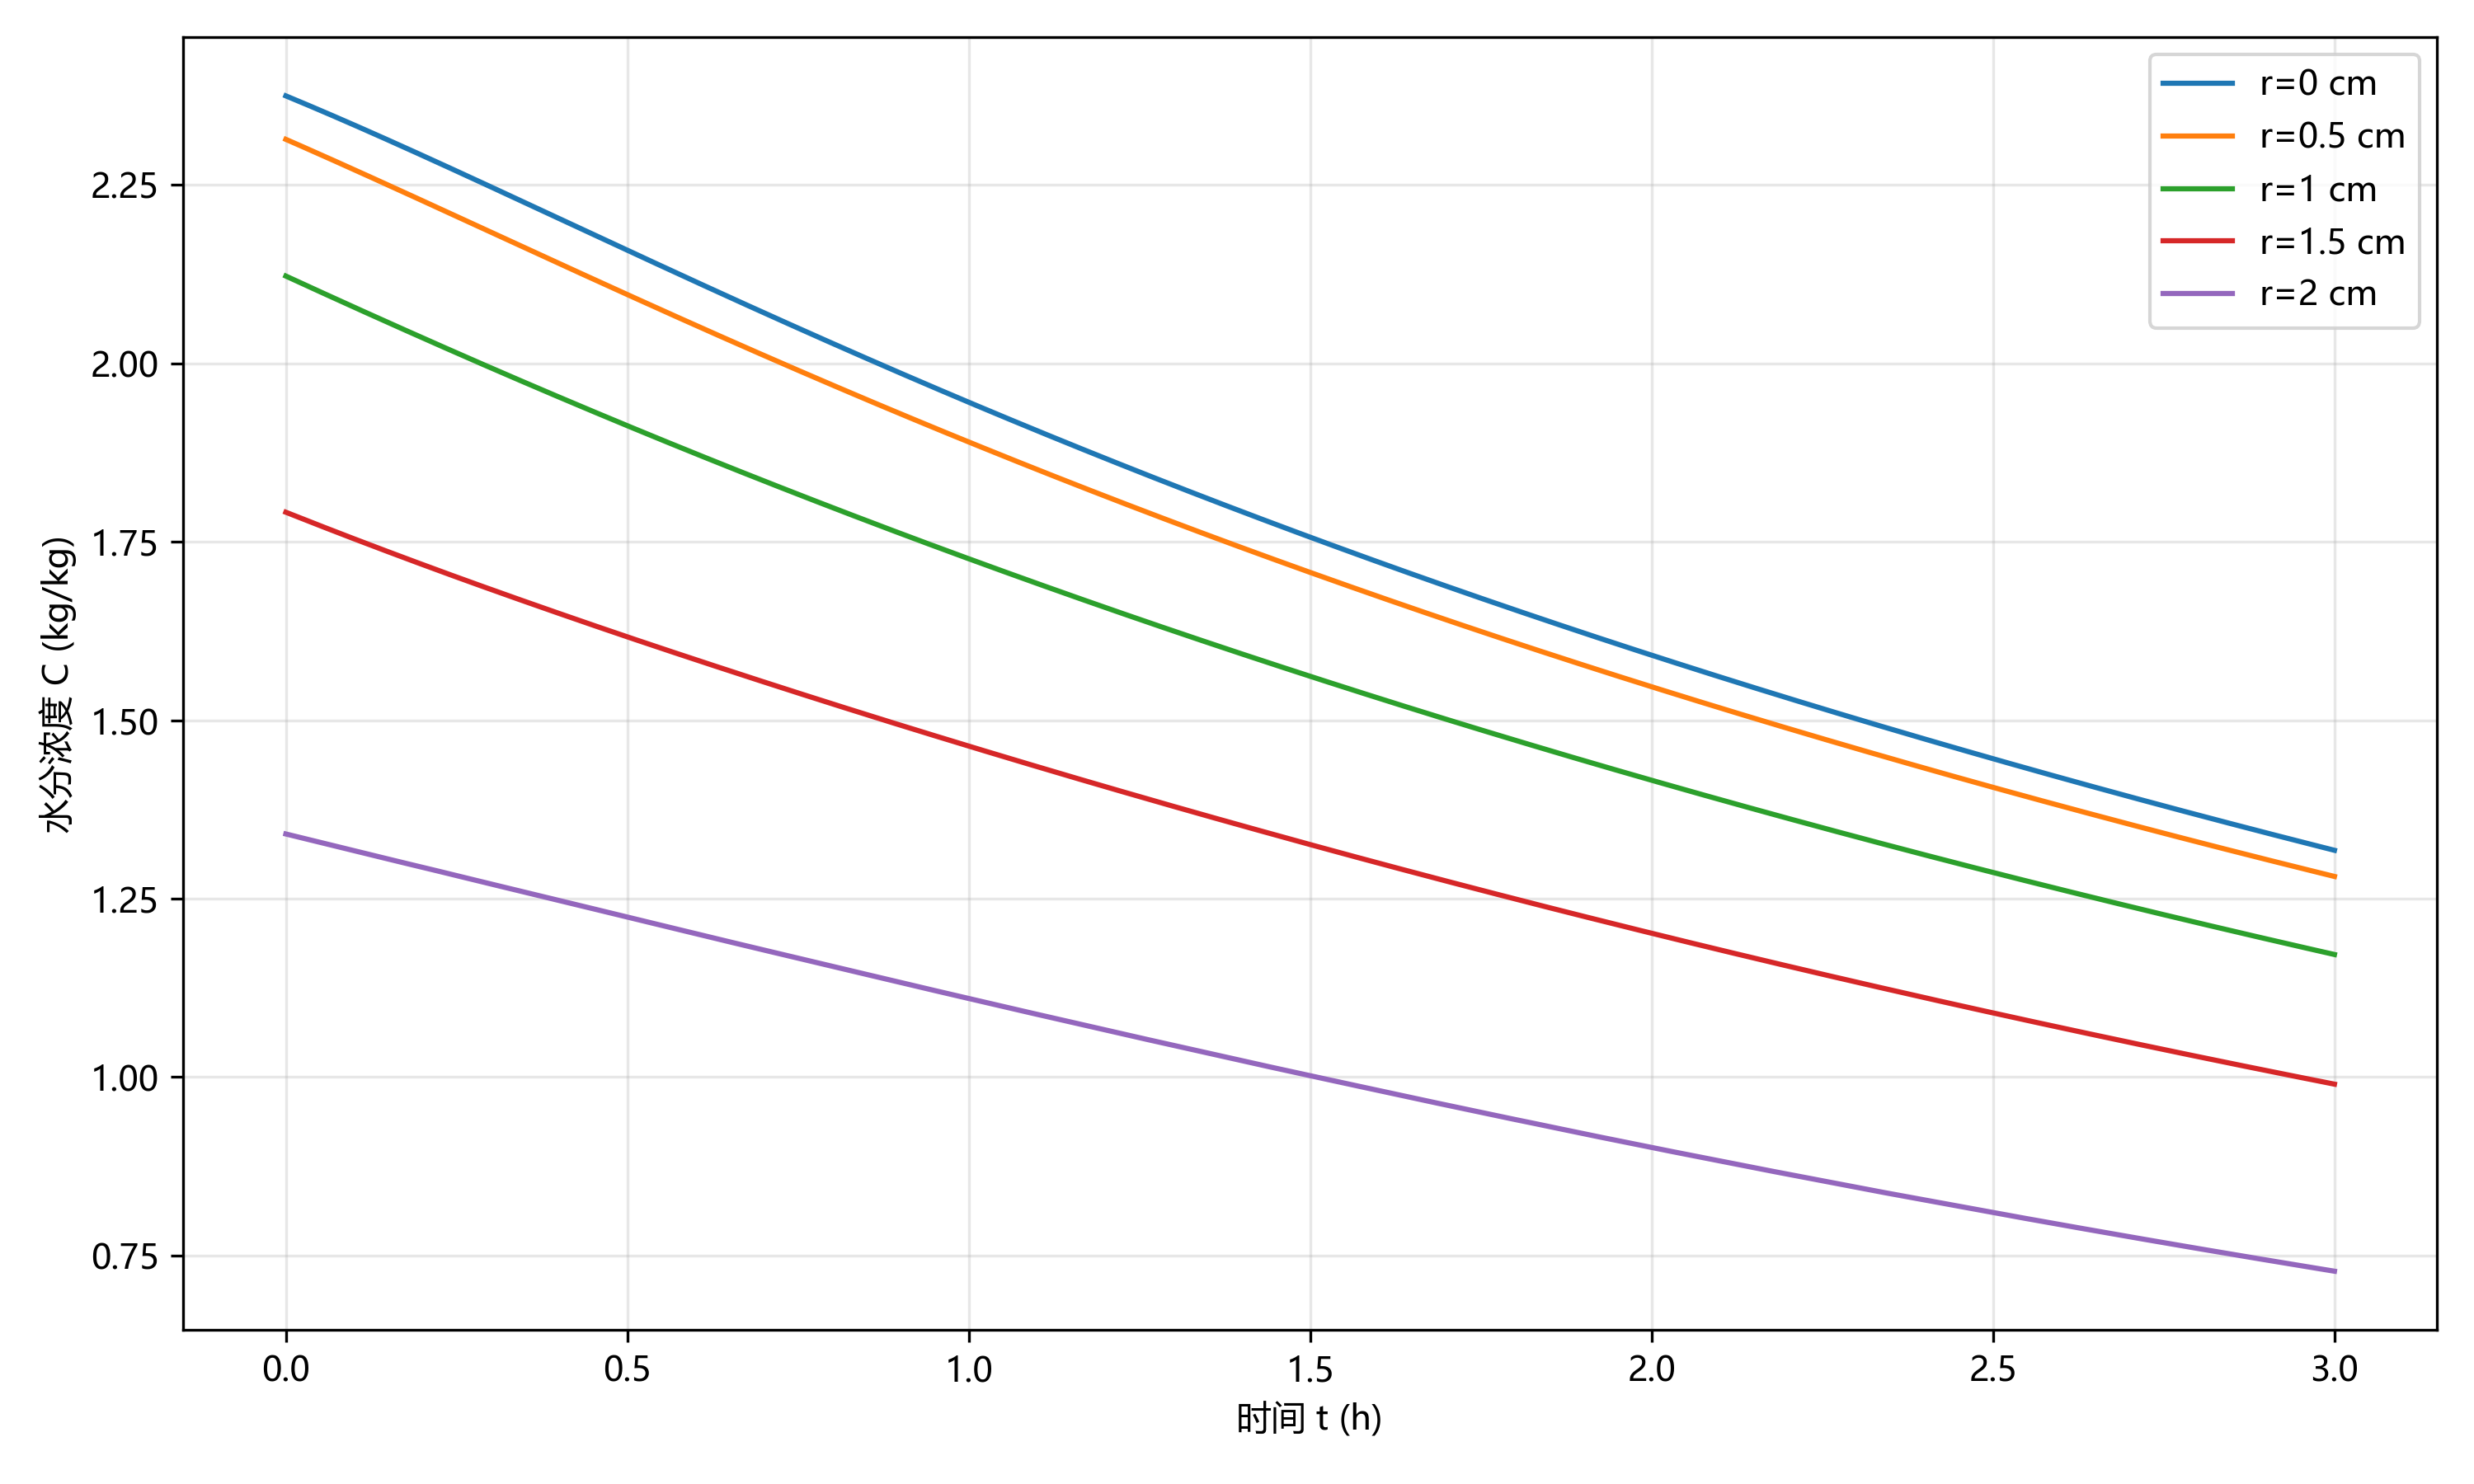
\includegraphics[width=0.5\linewidth]{pic/q2_水分时间演化图.png}
    \caption{问题二水分浓度随时间的变化}
    \label{fig:q2_moisture_time}
\end{figure}

\begin{figure}
    \centering
    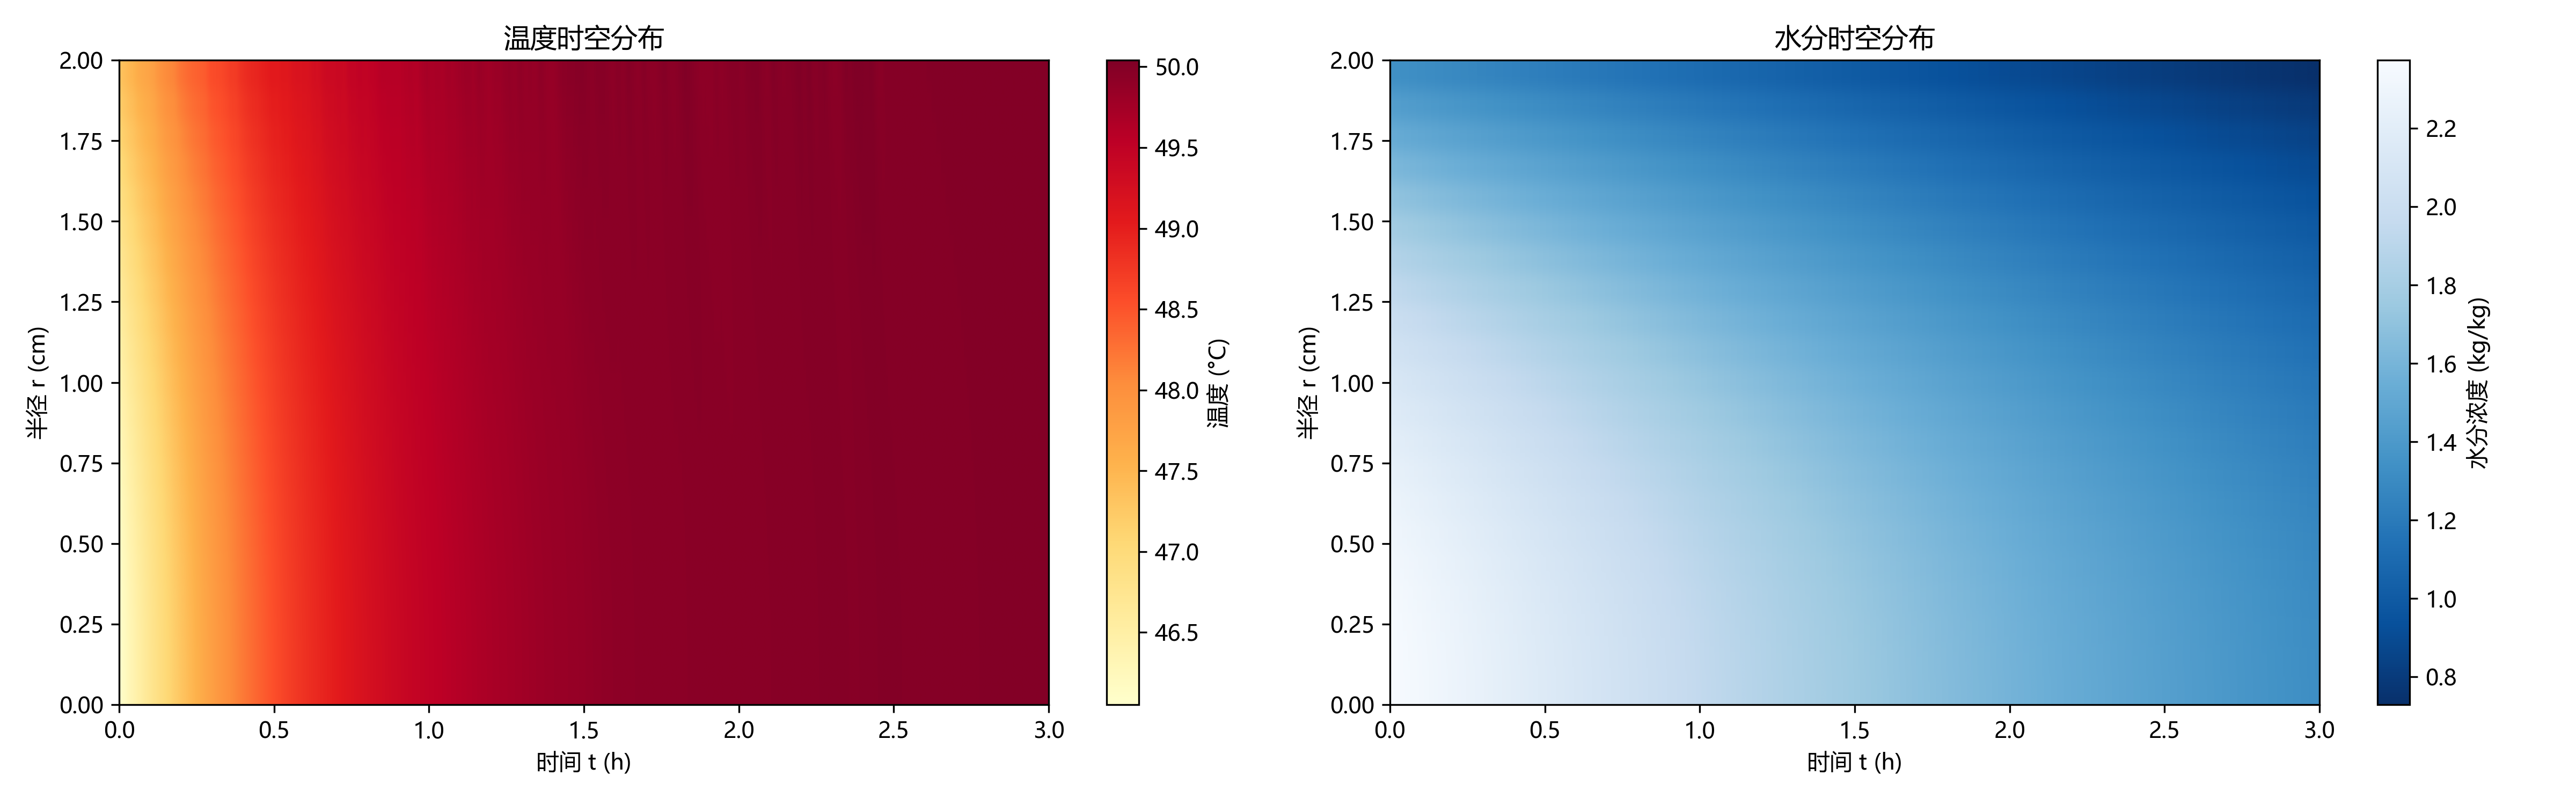
\includegraphics[width=0.5\linewidth]{pic/q2_温度和水分热力图.png}
    \caption{问题二温度和水分浓度热力图}
    \label{fig:q2_heatmap}
\end{figure}

\begin{figure}
    \centering
    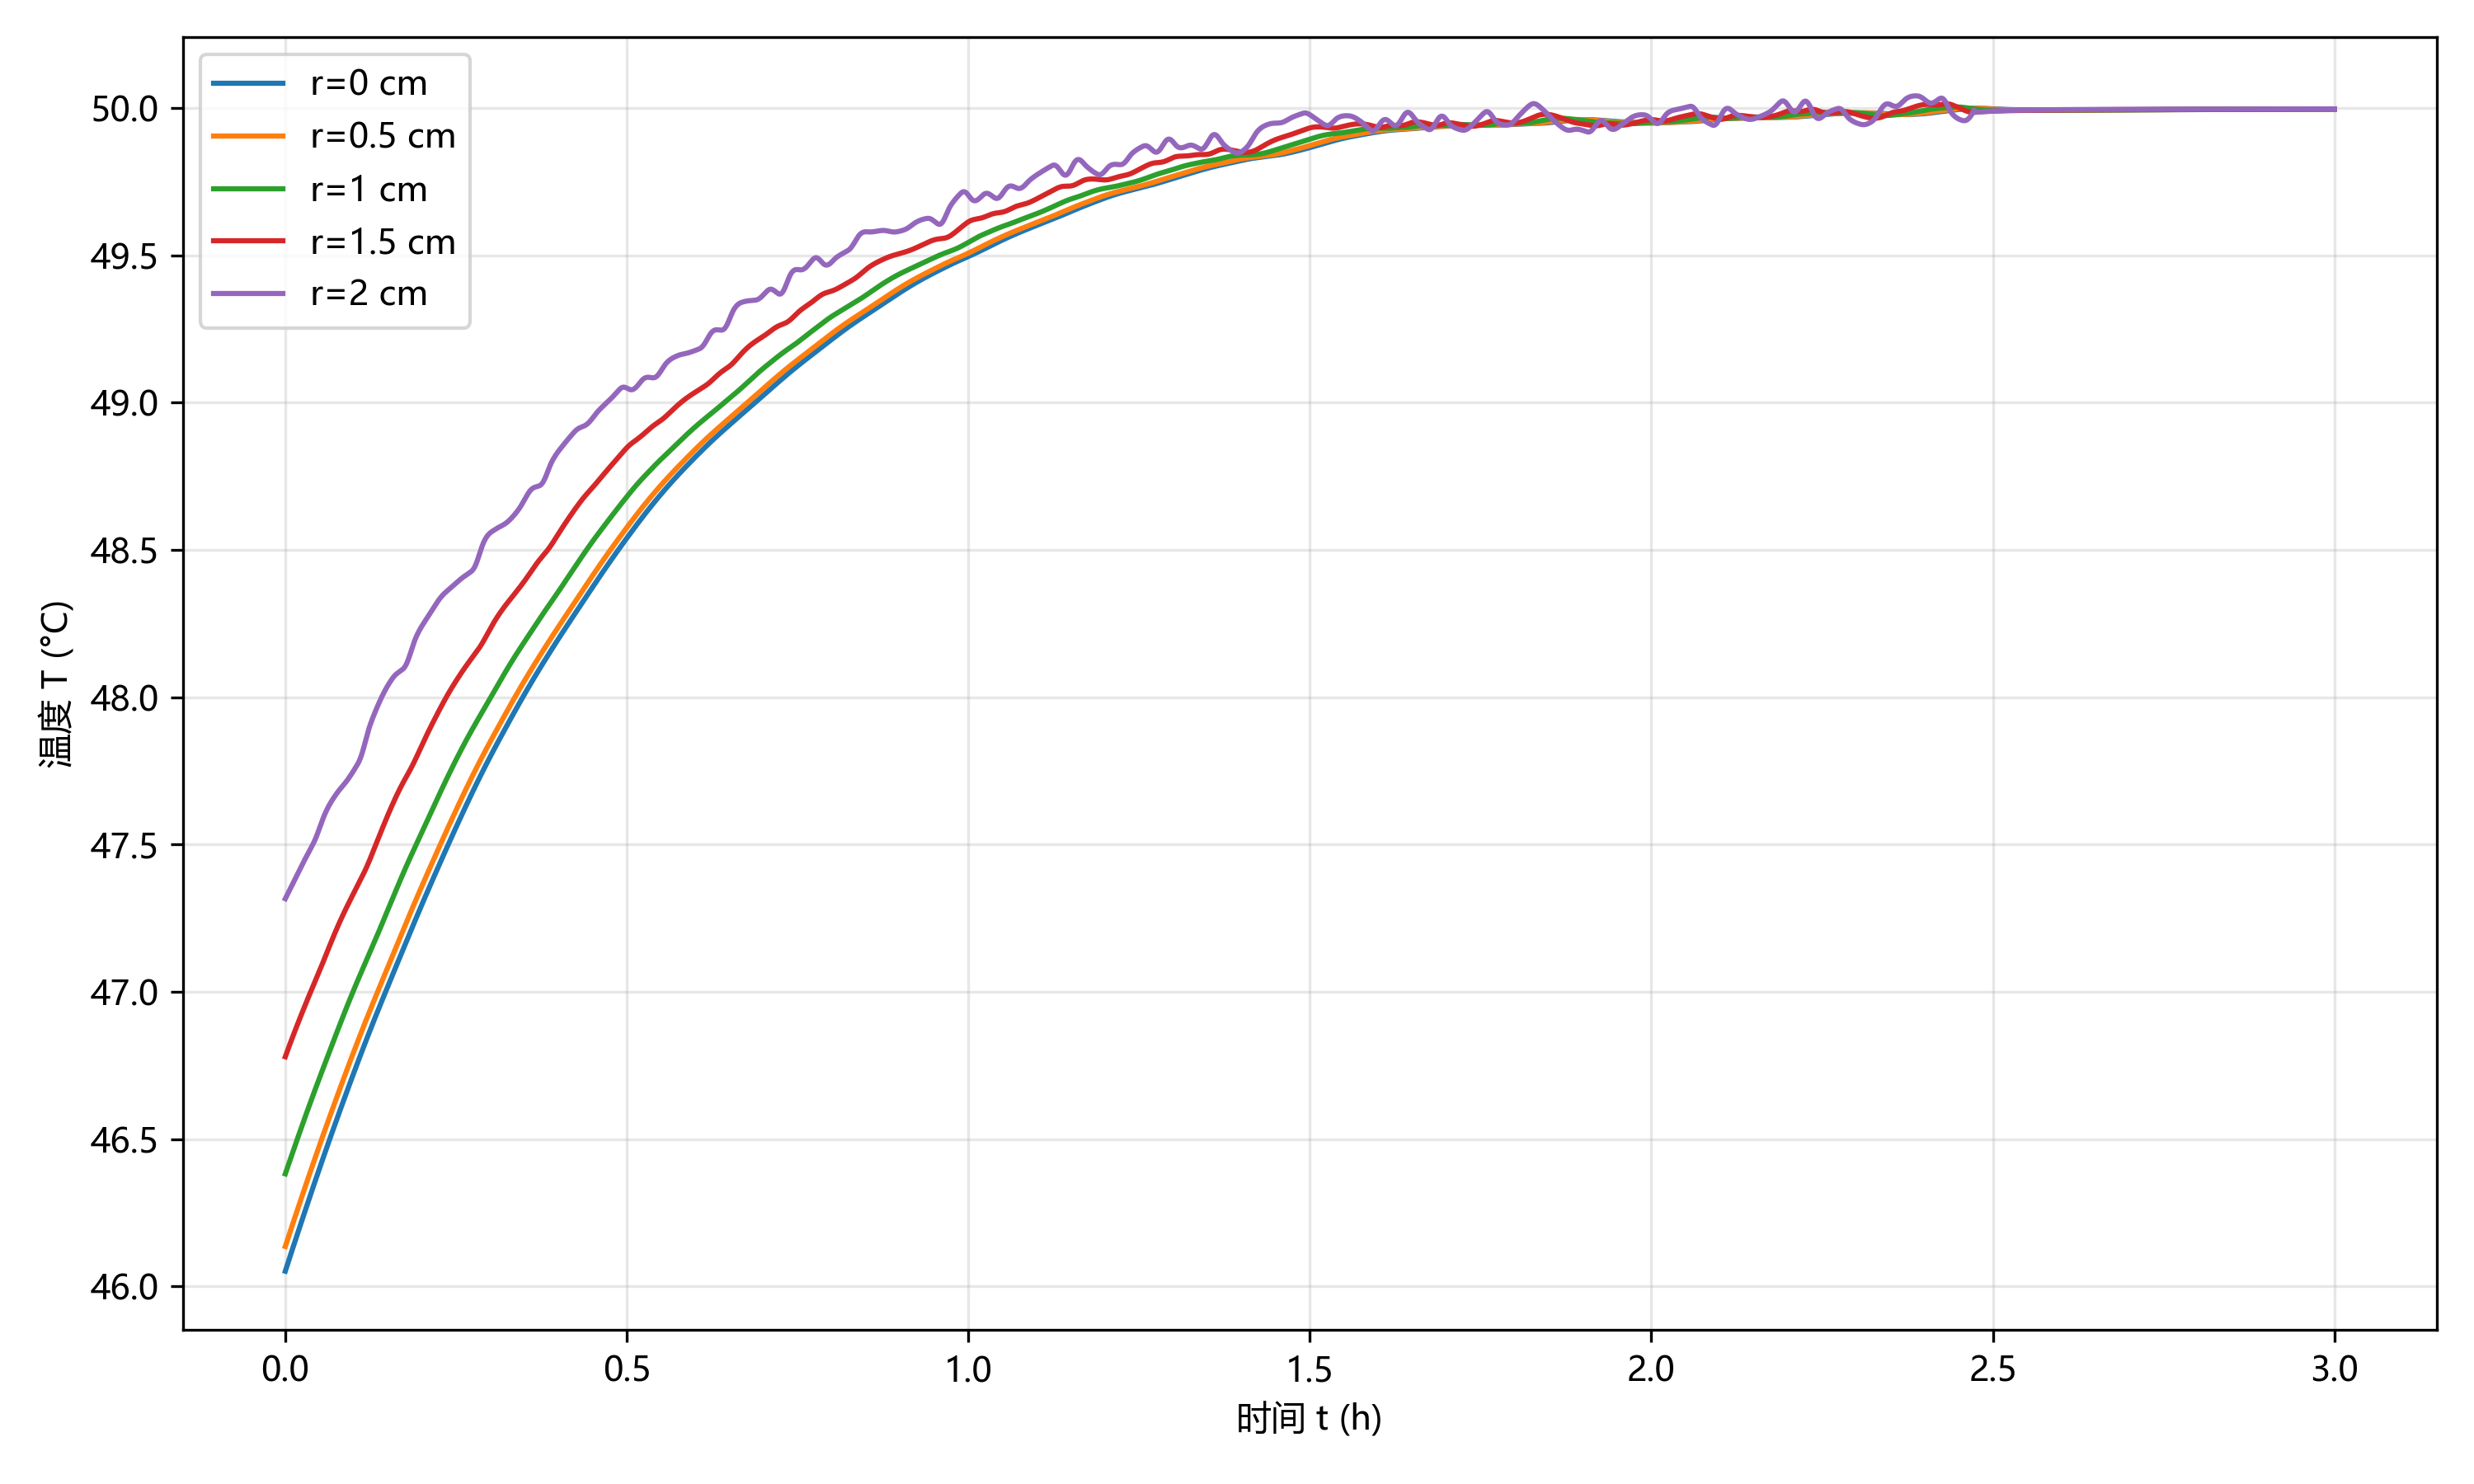
\includegraphics[width=0.5\linewidth]{pic/q2_温度时间演化图.png}
    \caption{问题二温度随时间的变化}
    \label{fig:q2_temperature_time}
\end{figure}

\begin{figure}
    \centering
    \IfFileExists{pic/q2_问题二的时空演化图.png}{%
      \includegraphics[width=0.5\linewidth]{pic/q2_问题二的时空演化图.png}%
    }{\PackageWarning{paper}{Missing figure pic/q2_问题二的时空演化图.png; skipped}}
    \caption{问题二的时空演化图}
    \label{fig:q2_spatiotemporal}
\end{figure}









%%%%%%%%%%%%%%%%%%%%%%%%%%%%%%%%%%%%%%%%%%%%%%%%%%%%%%%%%%%%% 
\newpage
\section{问题三：全过程固定半径模型的建立与求解}
\subsection{模型建立}

问题三沿用问题二的固定半径假设与附录 3 的变物性关系，即
\begin{equation}
R(t) \equiv R_0 = 0.02\,\text{m},
\end{equation}
且物性参数 \(\rho(C), c_p(C), k(C)\) 与扩散系数 \(D(C,T)\) 的表达式与问题二完全一致。所不同的是，问题三不再将 \(5500\,\text{s}\) 之后的阶段作为新的初值问题处理，而是从 \(t = 0\) 的原始均匀状态出发，直接计算至烘干结束。因此，环境边界使用统一建模框架中定义的拼接边界 \(B(t)\)，即
\begin{equation}
B(t) = 
\begin{cases}
(T_1(t), C_1(t)), & 0 \le t \le t_s, \\
(T_2(t), C_2(t)), & t > t_s,
\end{cases}
\end{equation}
其中 \(t_s = 5500\,\text{s}\)，\(T_1, C_1\) 为附件 1 的变化边界，\(T_2, C_2\) 为稳定阶段边界。控制方程、中心对称条件与表面 Robin 条件均与问题二相同，此处不再重复。

\subsection{全过程求解}

问题三采用与问题二相同的系数滞后后向 Euler 半隐式控制体格式，但时间步长取 \(\Delta t = 60\,\text{s}\)，空间步长仍为 \(\Delta r = 0.001\,\text{m}\)。最大绝对计算时间设为
\begin{equation}
t_{\max} = 259200\,\text{s} = 72\,\text{h}.
\end{equation}
每一步使用绝对时间查询拼接后的环境边界值 \(T_\infty^{n+1}\) 与 \(C_\infty^{n+1}\)，初值为
\begin{equation}
T_i^0 = 28^\circ\text{C}, \qquad C_i^0 = 2.55\,\text{kg/kg}, \qquad i = 0,1,\dots,N_r-1.
\end{equation}
温度与水分的三对角方程组形式与问题二完全一致，此处直接引用。

\subsection{烘干结束判据}

根据题意，药材内部各处的水分浓度均应低于 \(0.15\,\text{kg/kg}\)。为判断烘干是否结束，定义各时刻药材内部水分浓度的最大值为
\begin{equation}
C_{\max}(t_n) = \max_{0 \le i \le N_r-1} C_i^n.
\end{equation}
取首次满足 \(C_{\max}(t_j) \le 0.15\) 的网格时刻作为阈值跨越点。若上一时刻仍有 \(C_{\max}(t_{j-1}) > 0.15\)，则在区间 \([t_{j-1}, t_j]\) 上对 \(C_{\max}\) 进行线性插值，得到精确的烘干结束时间
\begin{equation}
t_d = t_{j-1} + \frac{0.15 - C_{\max}(t_{j-1})}{C_{\max}(t_j) - C_{\max}(t_{j-1})} (t_j - t_{j-1}).
\end{equation}

程序按 \(60\,\text{s}\) 保存全过程结果，并在末尾追加 \(t_d\) 对应的线性插值行；论文用表按每 \(6\,\text{h}\) 及结束时刻提取。本次计算首次达到阈值的时间为
\begin{equation}
t_d = 210634.7398\,\text{s} = 58.50965\,\text{h}.
\end{equation}

\subsection{求解结果}

\begin{table}[htbp]
    \centering
    % 表格标题，加粗，字号稍大
    \textbf{\large 表 5\quad 药材烘干过程的水分浓度}
    \vspace{5mm} % 标题与表格的间距
    
    % 增加行高，使表格更美观，与原图一致
    \renewcommand{\arraystretch}{1.6}
    
    % 定义表格列：共6列，全部居中，且有竖线边框

 \begin{tabular}{|c|c|c|c|c|c|}
         \hline
        % 第一行：合并前两行的“时间/h”，合并后五列的“到药材中心距离/cm”
        \multirow{2}{*}{时间/h} & \multicolumn{5}{c|}{到药材中心距离/cm} \\
        \cline{2-6} % 在第2到第6列画横线
        % 第二行：空出第一列，填写距离表头
         & 0 & 0.5 & 1 & 1.5 & 2 \\
        \hline
        % 数据部分
        6 & 1.0186 & 0.9897 & 0.903 & 0.7563 & 0.5342 \\
        \hline
        12 & 0.4568 & 0.4437 & 0.4036 & 0.3302 & 0.1651 \\
        \hline
        18 & 0.2992 & 0.2919 & 0.2692 & 0.226 & 0.0843 \\
        \hline
        % 使用省略号代替中间的行数据（24, 30, 36, 42, 48, 54）
        \dots & & & & & \\
        \hline
        % 对应 Excel 中时间 58.5096 的那一行数据
        烘干结束时间 & 0.15 & 0.1478 & 0.1406 & 0.126 & 0.0525 \\
        \hline
    \end{tabular}
\end{table}


\begin{figure}
    \centering
    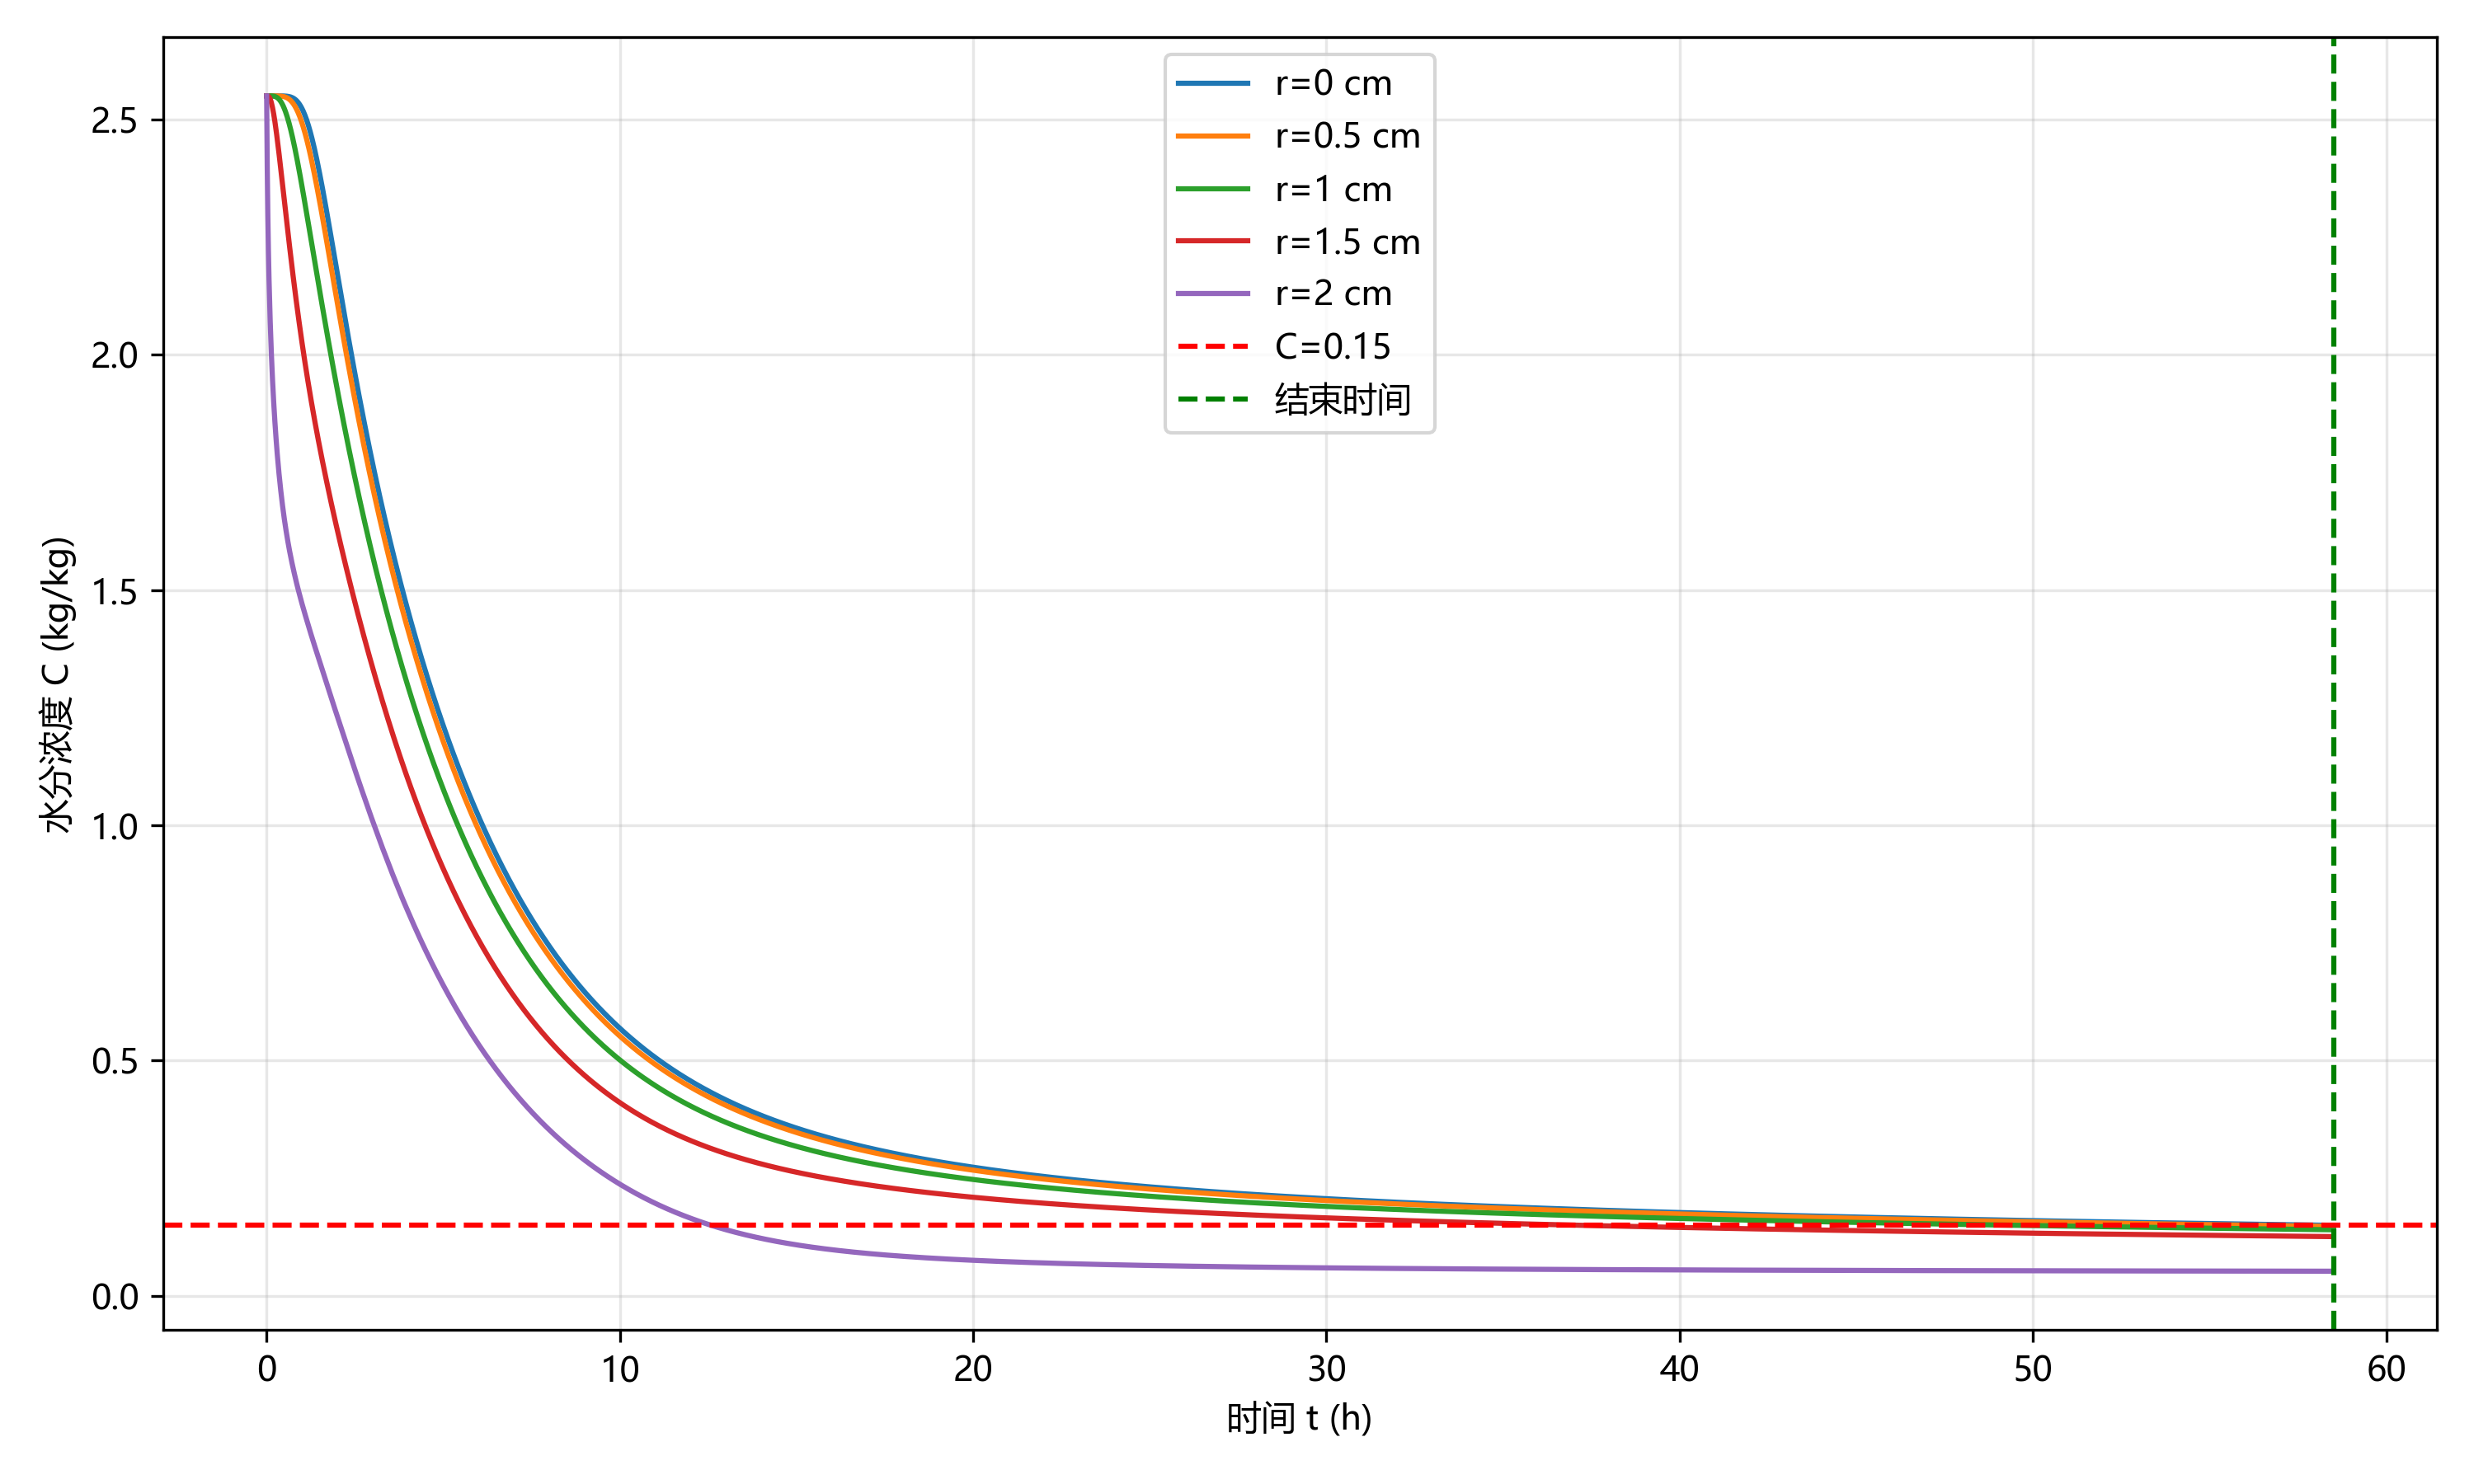
\includegraphics[width=0.5\linewidth]{pic/q3_水分时间演化图.png}
    \caption{问题三水分浓度随时间的变化}
    \label{fig:q3_moisture_time}
\end{figure}


\begin{figure}
    \centering
    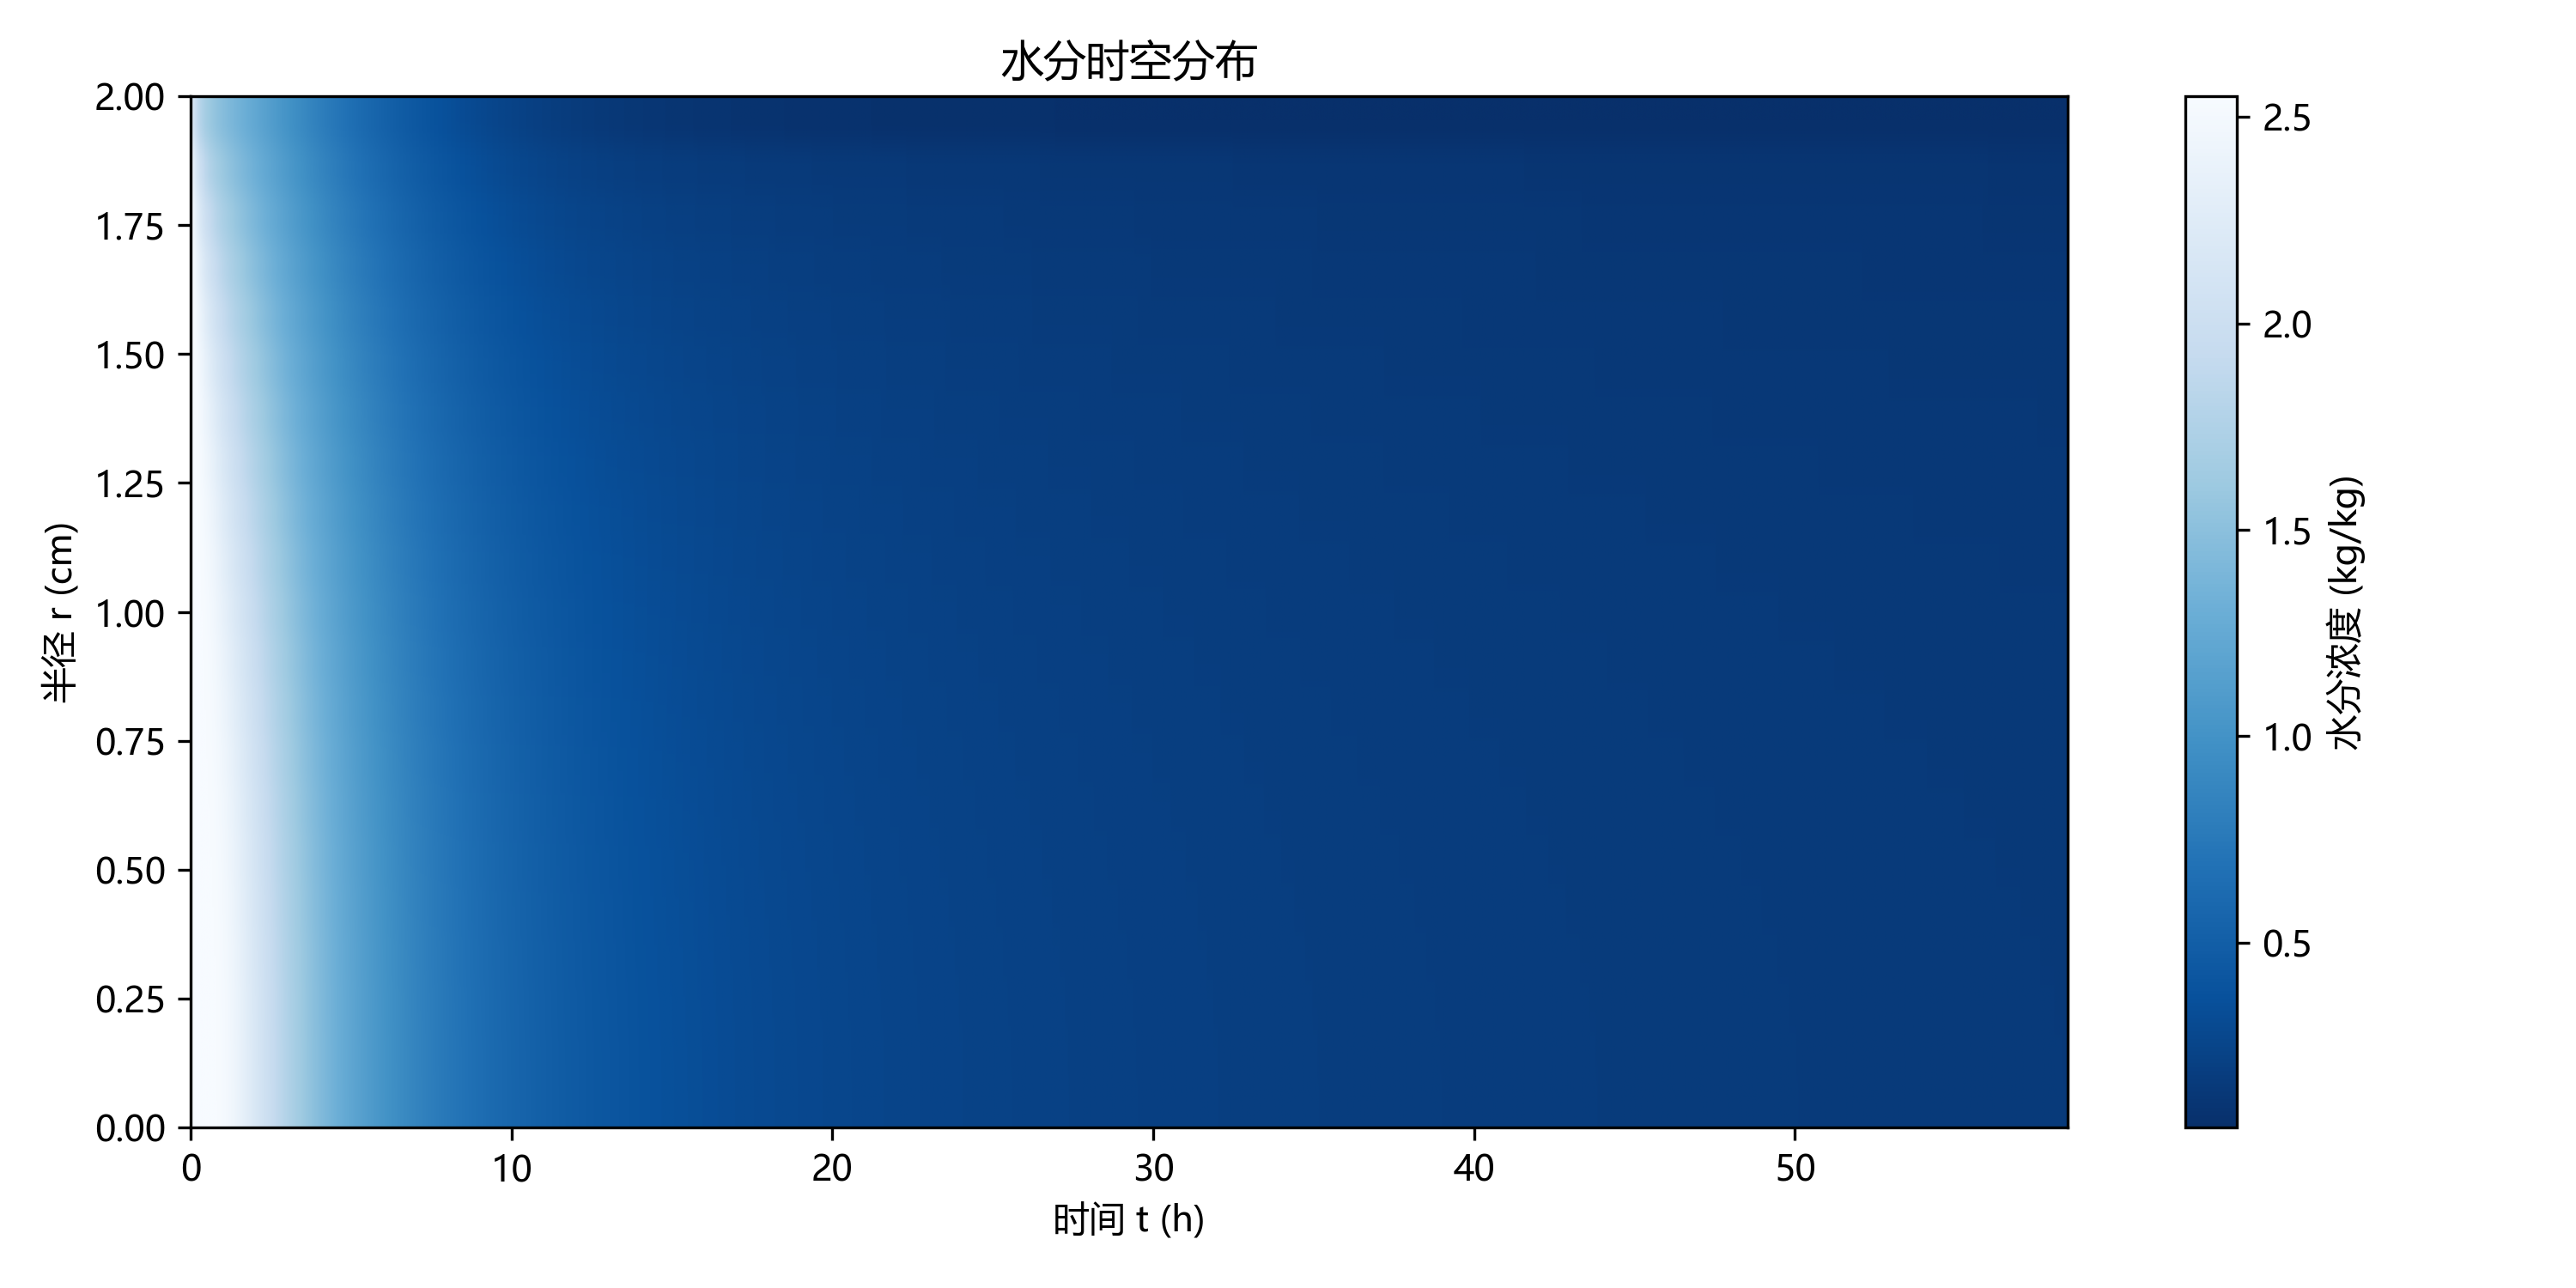
\includegraphics[width=0.5\linewidth]{pic/q3_水分热力图.png}
    \caption{问题三水分浓度热力图}
    \label{fig:q3_heatmap}
\end{figure}

\begin{figure}
    \centering
    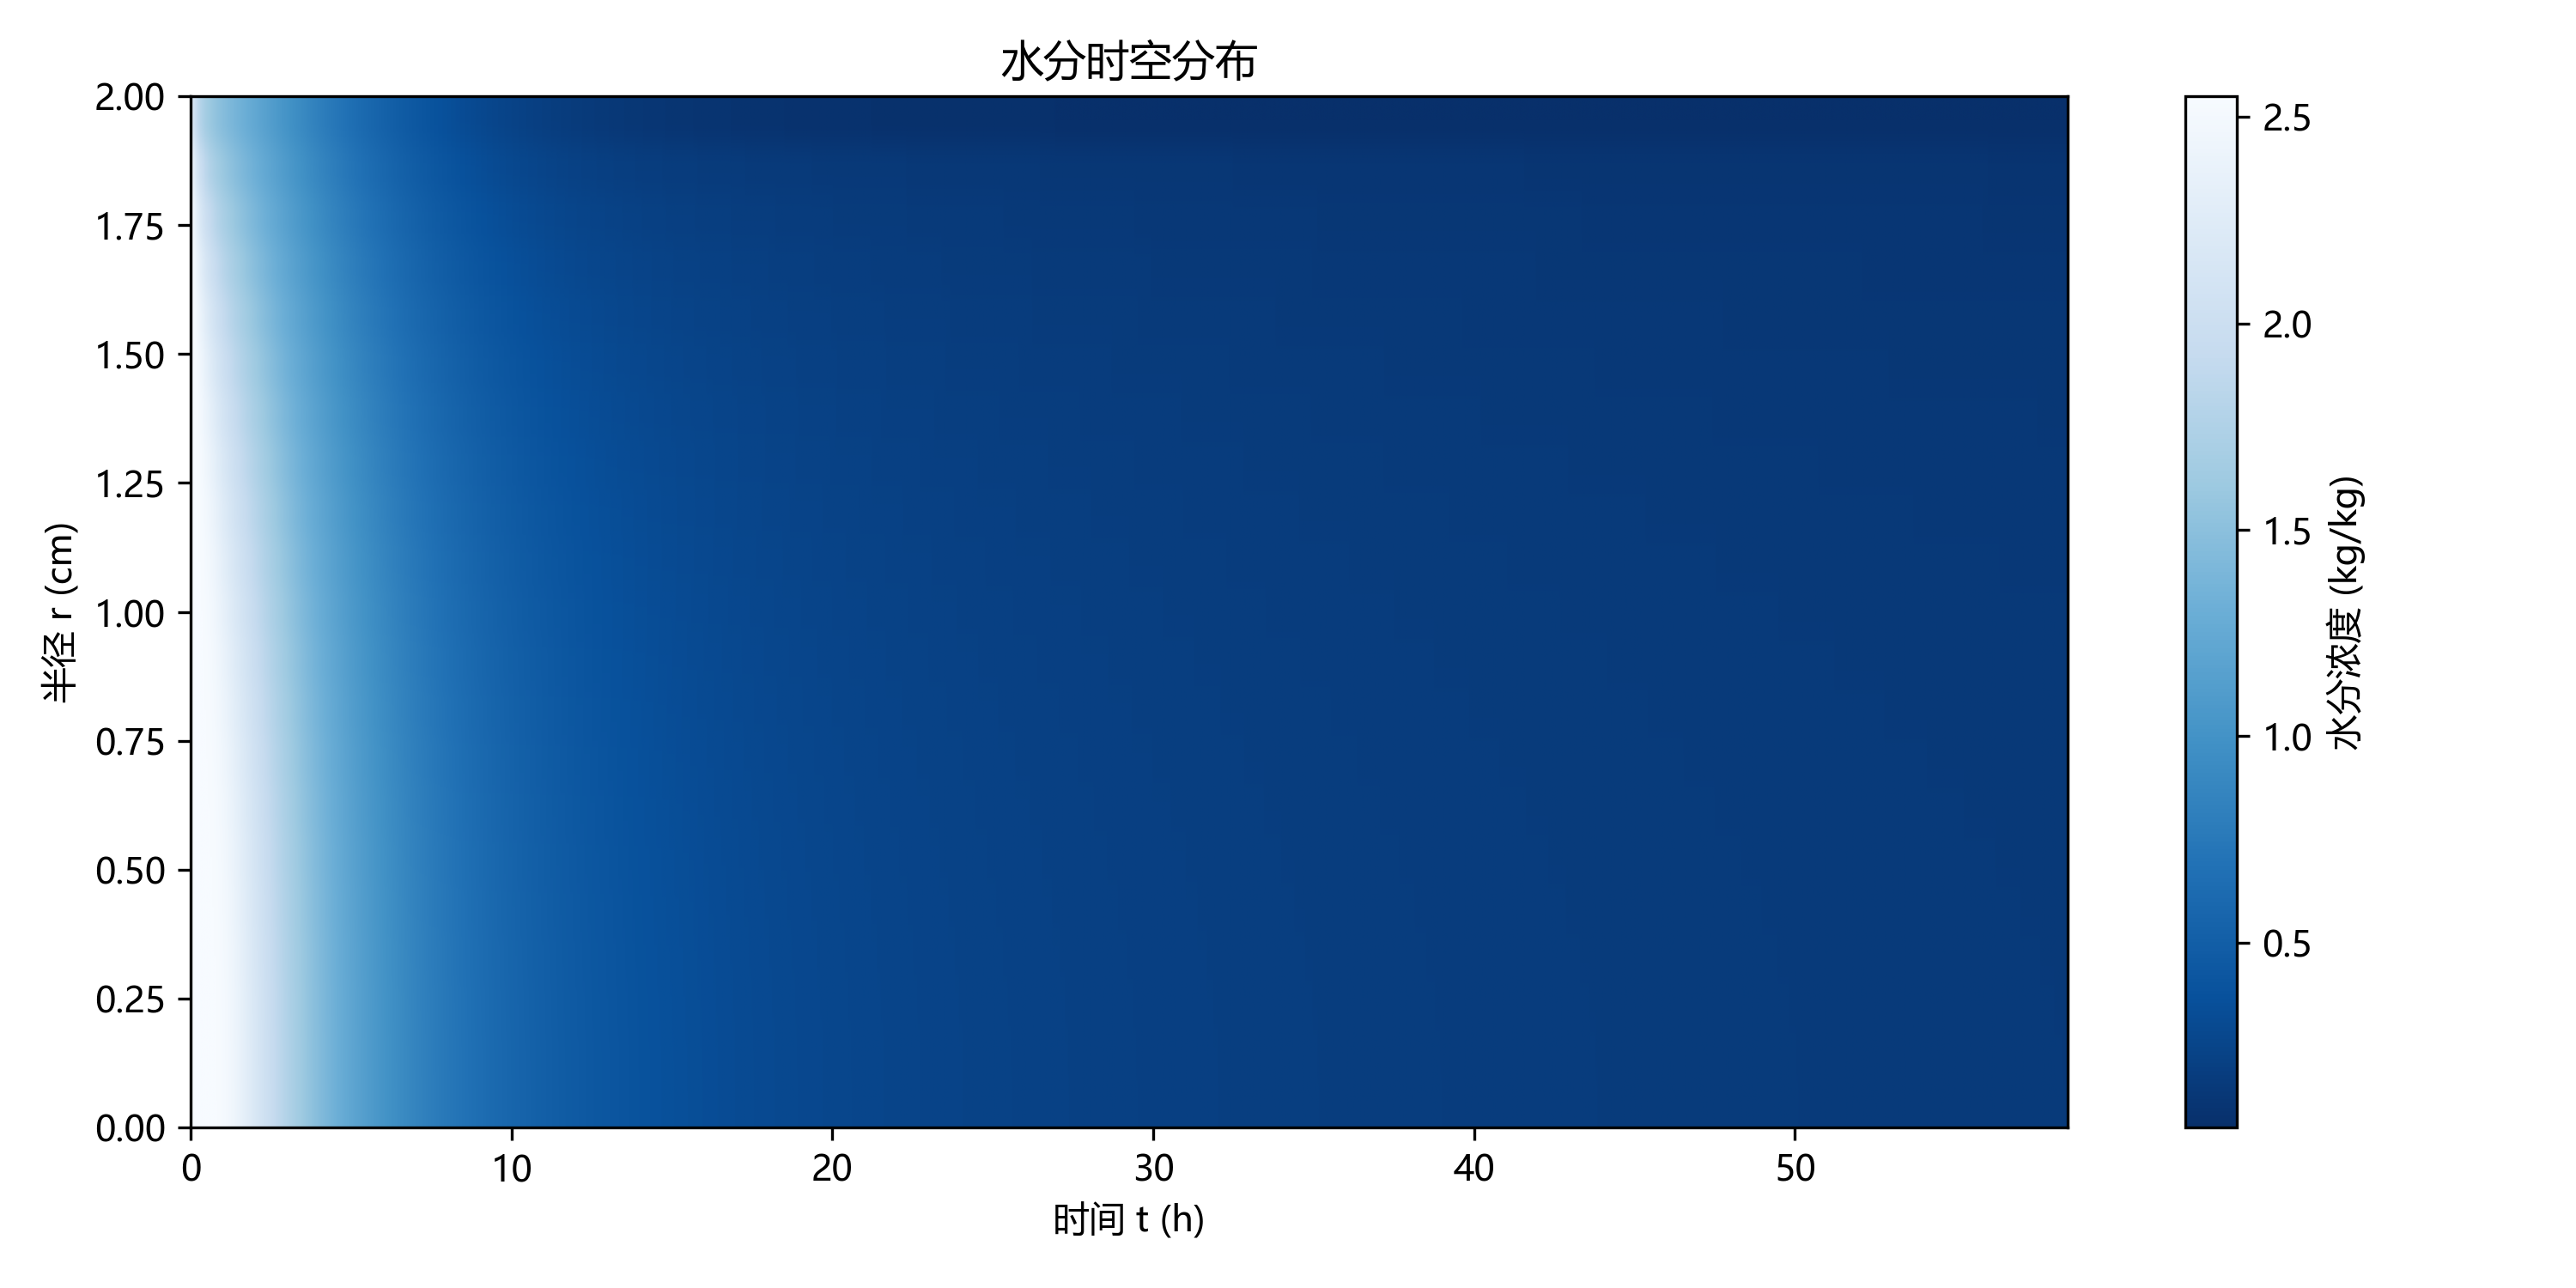
\includegraphics[width=0.5\linewidth]{pic/q3_水分热力图.png}
    \caption{问题三水分浓度热力图（重复绘制）}
    \label{fig:q3_heatmap_duplicate}
\end{figure}

\begin{figure}
    \centering
    \IfFileExists{pic/q3_达到干燥标准前后的径向含水率.png}{%
      \includegraphics[width=0.5\linewidth]{pic/q3_达到干燥标准前后的径向含水率.png}%
    }{\PackageWarning{paper}{Missing figure pic/q3_达到干燥标准前后的径向含水率.png; skipped}}
    \caption{问题三达到干燥标准前后的径向含水率}
    \label{fig:q3_radial}
\end{figure}



\begin{figure}
    \centering
    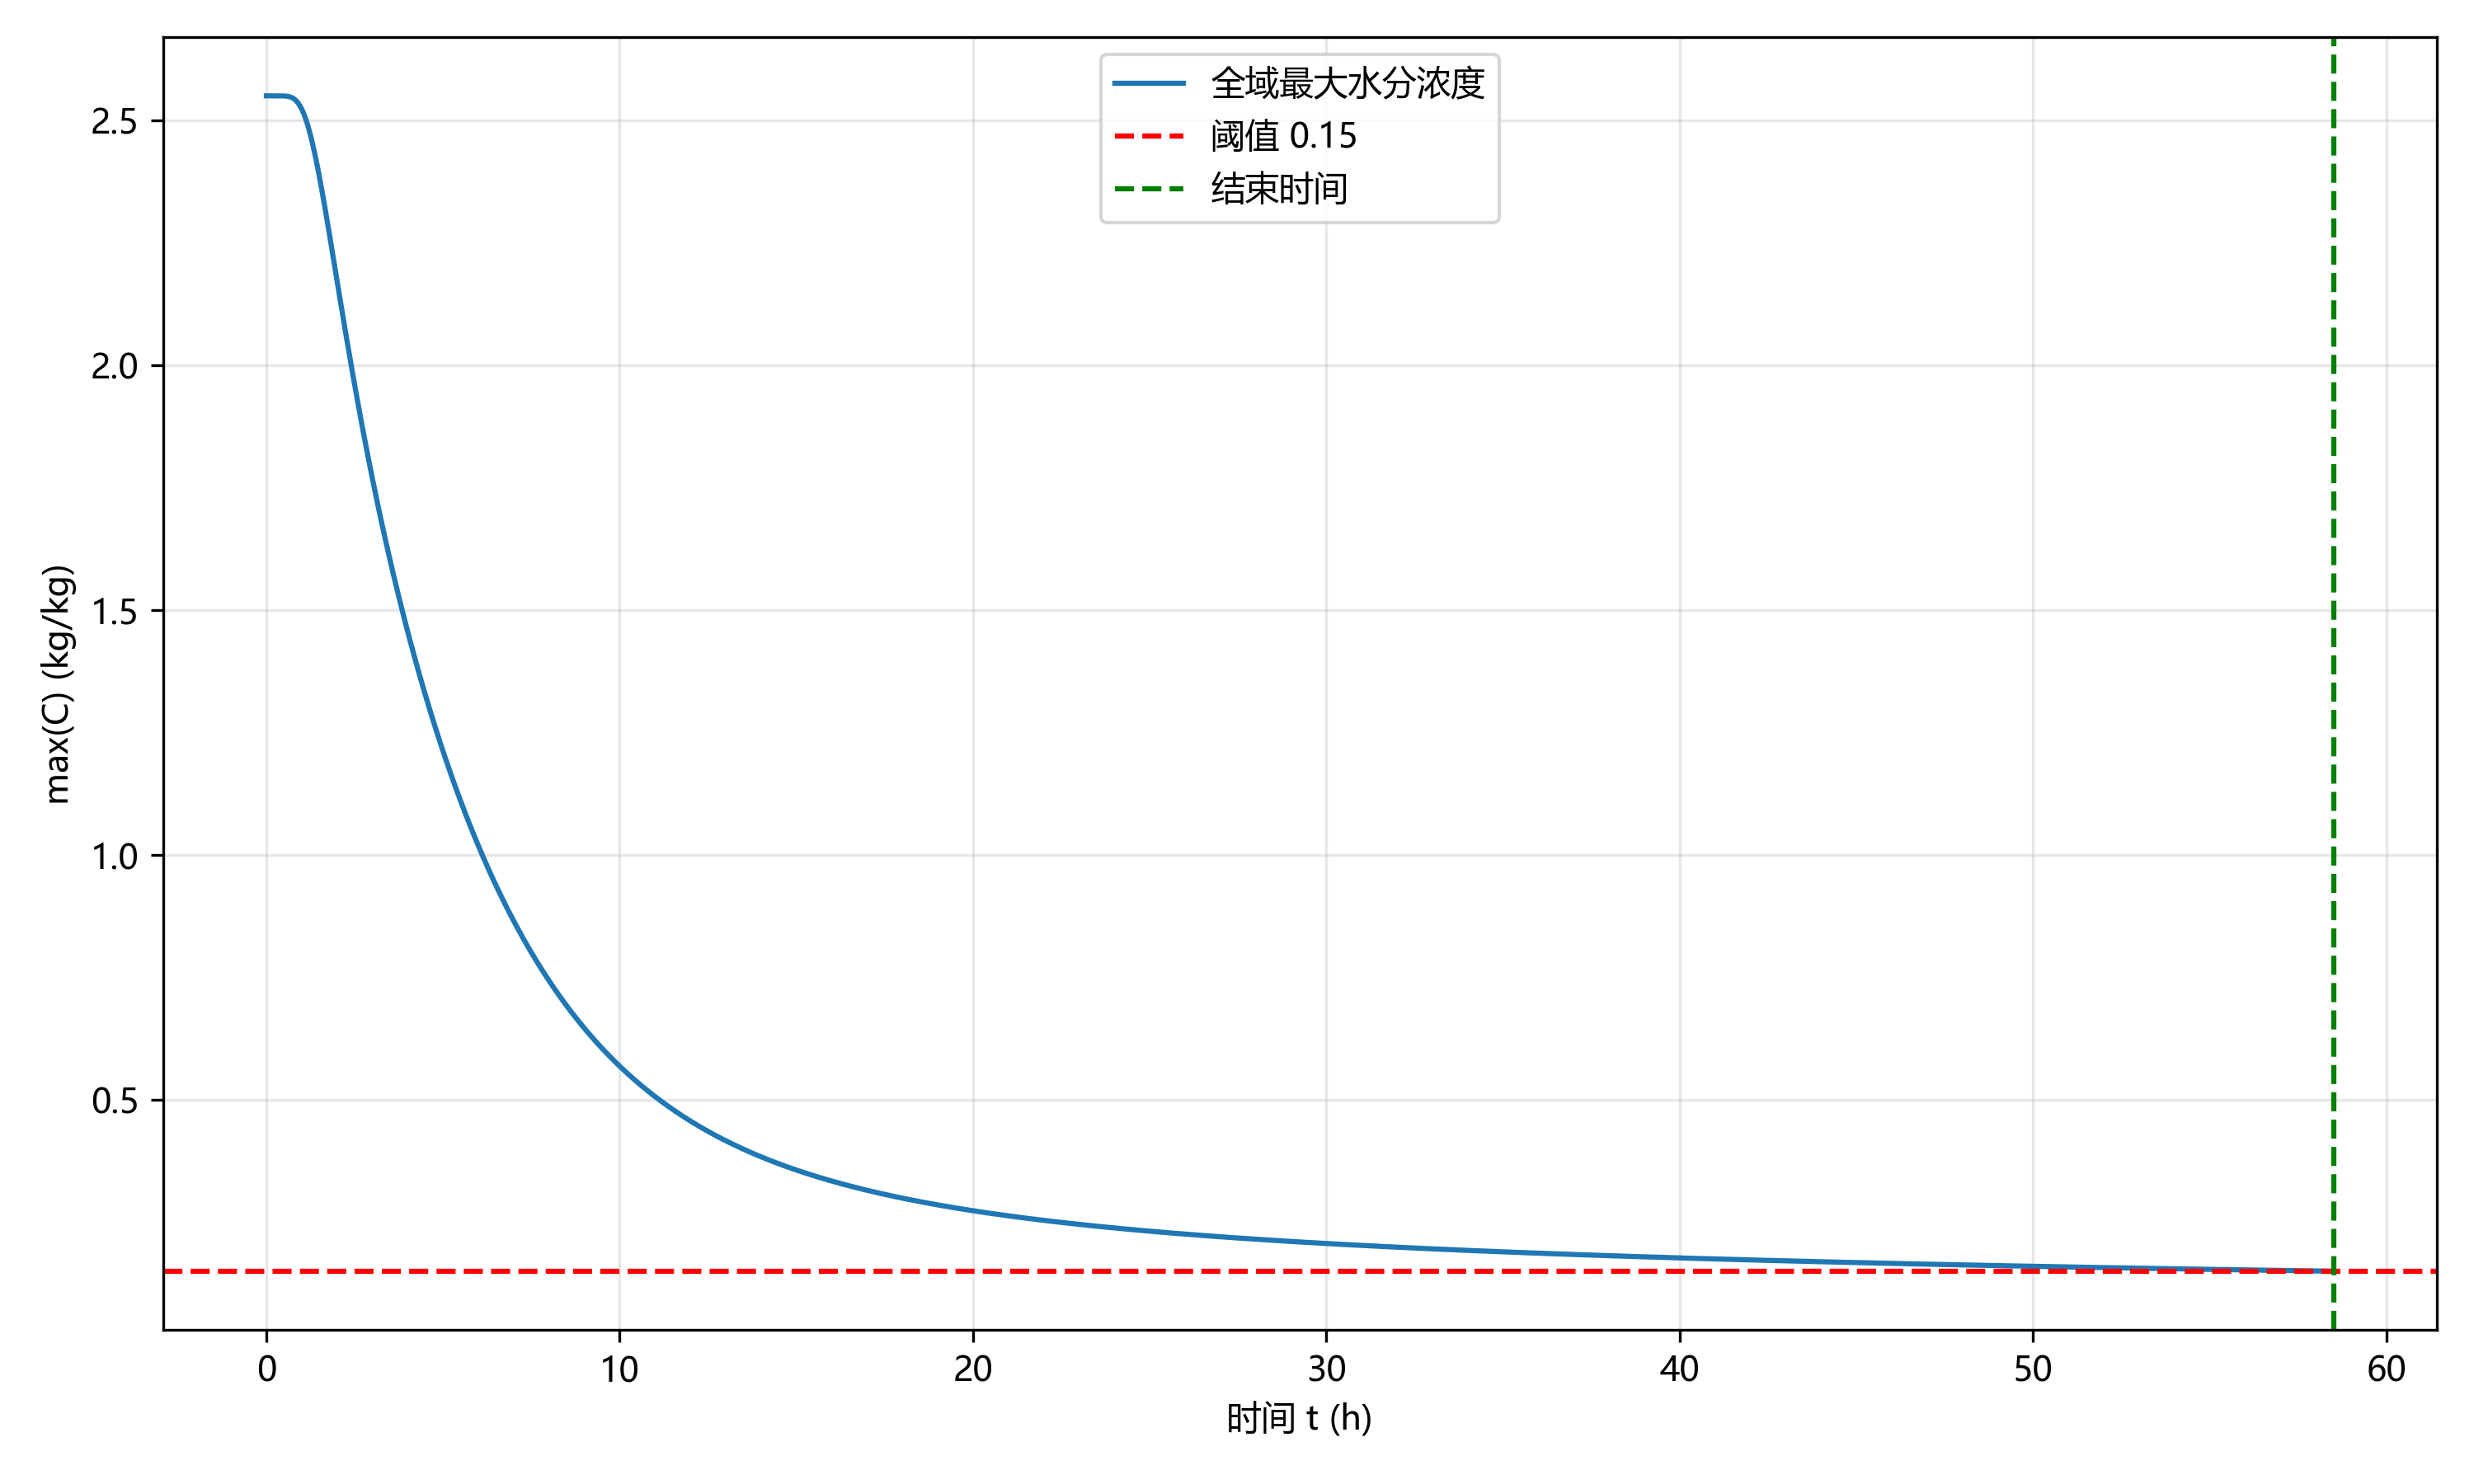
\includegraphics[width=0.5\linewidth]{pic/q3_阈值判定图.png}
    \caption{问题三干燥阈值判定}
    \label{fig:q3_threshold}
\end{figure}




按照上述模型与判据，程序输出 \(0 \sim t_d\) 内每隔 \(60\,\text{s}\)、径向每隔 \(0.1\,\text{cm}\) 的完整水分浓度结果，并按表 5 的格式给出每隔 \(6\,\text{h}\)、距药材中心每隔 \(0.5\,\text{cm}\) 的水分浓度。由计算结果可知，药材各处水分浓度均低于 \(0.15\,\text{kg/kg}\) 所需的时间约为 \(58.51\,\text{h}\)，即约 \(2.44\) 天，符合题目中烘干过程持续 \(2\sim3\) 天的实际情形。



























%%%%%%%%%%%%%%%%%%%%%%%%%%%%%%%%%%%%%%%%%%%%%%%%%%%%%%%%%%%%% 

\section{问题四：变半径材料坐标模型}

\subsection{移动边界与材料坐标}

问题一至问题三均假设药材半径 \(R\) 为常数。然而在实际烘干过程中，药材因水分流失会发生明显的体积收缩。此时计算区域不再是固定的 \(0 \le r \le R\)，而是随时间变化的移动边界区域 \(0 \le r \le R(t)\)。问题四使用附件 2 给出的半径数据 \(R(t)\)，并假设药材沿径向均匀收缩。为将移动边界问题转化为固定区域上的问题，定义材料坐标
\begin{equation}
\xi = \frac{r}{R(t)}, \qquad 0 \le \xi \le 1.
\end{equation}
固定 \(\xi\) 表示随骨架运动的同一材料位置。对任意场变量 \(u(r,t) = \tilde{u}(\xi,t)\)，由链式法则有
\begin{equation}
\left.\frac{\partial u}{\partial r}\right|_t = \frac{1}{R(t)}\frac{\partial \tilde{u}}{\partial \xi}.
\end{equation}
在该材料坐标描述下，沿材料点的时间变化率即为 \(\partial \tilde{u}/\partial t|_{\xi}\)。

附件 2 的半径数据先由 PCHIP 插值到计算网格 \(t_n = n\Delta t\)，得到 \(R_n = R(t_n)\)。程序再作累计最小值修正，仅消除浮点误差造成的局部极小上升，从而保证 \(R_{n+1} \le R_n\)。

\subsection{变半径控制方程与边界条件}

问题四使用附录 4 给出的物性关系：
\begin{equation}
\rho(C) = 760 + 90C,
\end{equation}
\begin{equation}
c_p(C) = 1850 + 2150\frac{C}{C+1},
\end{equation}
\begin{equation}
k(C) = 0.12 + 0.20\frac{C}{C+1},
\end{equation}
\begin{equation}
D(C,T) = 4.2\times 10^{-4}\exp\left(-\frac{0.30}{C}\right)\exp\left(-\frac{3850}{T_K}\right),
\end{equation}
其中 \(T_K = T + 273.15\)。

将材料坐标变换代入统一建模框架中的守恒方程，可得固定材料坐标下的控制方程组：
\begin{equation}
\rho(\tilde{C})c_p(\tilde{C})\frac{\partial \tilde{T}}{\partial t} = \frac{1}{R(t)^2\xi}\frac{\partial}{\partial \xi}\left[\xi k(\tilde{C})\frac{\partial \tilde{T}}{\partial \xi}\right],
\end{equation}
\begin{equation}
\frac{\partial \tilde{C}}{\partial t} = \frac{1}{R(t)^2\xi}\frac{\partial}{\partial \xi}\left[\xi D(\tilde{C},\tilde{T})\frac{\partial \tilde{C}}{\partial \xi}\right].
\end{equation}

初始条件为
\begin{equation}
\tilde{T}(\xi,0) = 28^\circ\text{C}, \qquad \tilde{C}(\xi,0) = 2.55\,\text{kg/kg}, \qquad 0 \le \xi \le 1.
\end{equation}

中心对称条件为
\begin{equation}
\frac{\partial \tilde{T}}{\partial \xi}(0,t) = 0, \qquad \frac{\partial \tilde{C}}{\partial \xi}(0,t) = 0.
\end{equation}

在当前表面 \(\xi=1\) 处，Robin 边界条件为
\begin{equation}
-\frac{k(\tilde{C}_s)}{R(t)}\frac{\partial \tilde{T}}{\partial \xi}(1,t) = h\left[\tilde{T}_s - T_\infty(t)\right],
\end{equation}
\begin{equation}
-\frac{D(\tilde{C}_s,\tilde{T}_s)}{R(t)}\frac{\partial \tilde{C}}{\partial \xi}(1,t) = h_m\left[\tilde{C}_s - C_\infty(t)\right],
\end{equation}
其中 \(\tilde{T}_s = \tilde{T}(1,t)\)，\(\tilde{C}_s = \tilde{C}(1,t)\)。

\subsection{固定材料坐标控制体离散}

空间网格取 \(\xi_i = i\Delta\xi\)，\(\Delta\xi = 0.05\)，\(N_r = 21\)；时间步长 \(\Delta t = 60\,\text{s}\)。单位化后的控制体权重为
\begin{equation}
w_0 = \left(\frac{\Delta\xi}{2}\right)^2, \quad
w_i = 2\xi_i\Delta\xi \quad (1 \le i \le N_r-2), \quad
w_{N_r-1} = 1 - \left(1 - \frac{\Delta\xi}{2}\right)^2.
\end{equation}

为统一表示温度和水分，令 \(u\) 分别取 \(\tilde{T}\) 或 \(\tilde{C}\)，\(H_i^n\) 分别取 \(\rho(C_i^n)c_p(C_i^n)\) 或 1，\(q_{i+1/2}^n\) 分别取 \(k\) 或 \(D\)。界面位置与界面系数为
\begin{equation}
\xi_{i+1/2} = \left(i + \frac{1}{2}\right)\Delta\xi,
\end{equation}
\begin{equation}
q_{i+1/2}^n = 
\begin{cases}
k\left(\frac{C_i^n + C_{i+1}^n}{2}\right), & u = \tilde{T}, \\[4pt]
D\left(\frac{C_i^n + C_{i+1}^n}{2}, \frac{T_i^n + T_{i+1}^n}{2}\right), & u = \tilde{C}.
\end{cases}
\end{equation}

每个时间步使用 \(R_{n+1}\) 进入尺度因子与表面系数。对含有左右界面的控制体，后向 Euler 离散为
\begin{equation}
\begin{aligned}
\frac{H_i^n w_i}{\Delta t}(u_i^{n+1} - u_i^n) = \frac{2}{R_{n+1}^2} \Bigg[ &\xi_{i+1/2} q_{i+1/2}^n \frac{u_{i+1}^{n+1} - u_i^{n+1}}{\Delta\xi} \\
- &\xi_{i-1/2} q_{i-1/2}^n \frac{u_i^{n+1} - u_{i-1}^{n+1}}{\Delta\xi} \Bigg].
\end{aligned}
\end{equation}

中心控制体没有左界面通量，表面控制体没有右界面通量，且表面控制体额外增加对流项：
\begin{equation}
\begin{aligned}
\frac{H_s^n w_s}{\Delta t}(u_s^{n+1} - u_s^n) = &-\frac{2}{R_{n+1}}\xi_{s-1/2} q_{s-1/2}^n \frac{u_s^{n+1} - u_{s-1}^{n+1}}{\Delta\xi} \\
&+ \frac{2h_u}{R_{n+1}}\left(u_{\text{air}}^{n+1} - u_s^{n+1}\right),
\end{aligned}
\end{equation}
其中温度方程取 \((h_u, u_{\text{air}}) = (h, T_\infty)\)，水分方程取 \((h_u, u_{\text{air}}) = (h_m, C_\infty)\)。

上述方程逐控制体组装为三对角方程组，并使用追赶法求解。

\subsection{求解顺序}

问题四采用系数滞后的后向 Euler 半隐式格式，每个时间步的计算流程如图 \ref{fig:q4_flow} 所示。流程呈顺序结构，每步的输入均来自上一时刻的已知量，时间步内不进行非线性迭代。

\begin{figure}[H]
    \centering
    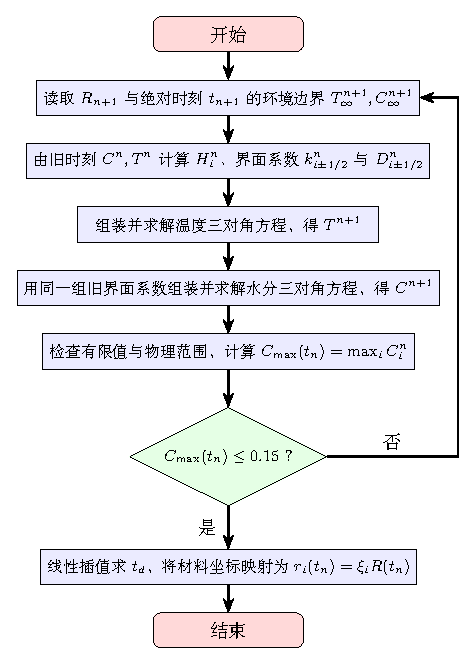
\includegraphics[width=0.6\linewidth]{pic/q4algorithm.pdf}
    \caption{算法求解顺序图}
    \label{fig:q4_flow}
\end{figure}

补充说明三点：其一，半径数据经 PCHIP 插值后作累计最小值修正，以保证 \(R_{n+1} \le R_n\)；其二，物性参数与界面系数均取旧时刻值，温度与水分方程共用，且步内不迭代；其三，输出位置按 \(r_i(t_n) = \xi_i R(t_n)\) 映射，超出当前半径则留空，并保存无量纲网格与半径插值表。

整个时间推进过程中，各步均为显式物性更新与线性方程组求解，不涉及迭代与反解，因此计算效率较高、实现简洁。

\subsection{求解结果}


\begin{table}[htbp]
    \centering
    % 表格标题，加粗，字号稍大
    \textbf{\large 表 6\quad 药材烘干过程的水分浓度}
    \vspace{5mm} % 标题与表格的间距
    
    % 增加行高，使表格更美观，与原图一致
    \renewcommand{\arraystretch}{1.6}
    
    % 定义表格列：共5列，全部居中，且有竖线边框
    \begin{tabular}{|c|c|c|c|c|}
        \hline
        \multirow{2}{*}{时间/h} & \multicolumn{4}{c|}{到药材中心的距离/cm} \\
        \cline{2-5}
         & 0 & 0.5 & 1 & 药材表面 \\
        \hline
        6 & 1.7182 & 1.536 & 1.0211 & 0.4205 \\
        \hline
        12 & 0.7377 & 0.6545 & 0.4079 & 0.1671 \\
        \hline
        18 & 0.4088 & 0.3686 & 0.2394 & 0.0891 \\
        \hline
        \dots & & & & \\
        \hline
        烘干结束时间 & 0.15 & 0.1413 & 0.1085 & 0.0526 \\
        \hline
    \end{tabular}
\end{table}



按全域水分阈值判定，本问得到烘干结束时间
\begin{equation}
t_d = 184815.7394\,\text{s} = 51.33771\,\text{h},
\end{equation}
此时药材半径由初始的 \(R(0) = 2.000\,\text{cm}\) 收缩至
\begin{equation}
R(t_d) = 1.198\,\text{cm}.
\end{equation}

与问题三在固定半径假设下得到的 \(58.51\,\text{h}\) 相比，考虑尺寸收缩后所需的烘干时间缩短至约 \(51.34\,\text{h}\)，减小了约 \(12\%\)。这一差异表明，药材收缩会缩短水分迁移路径并增大表面对流传质面积，从而加速干燥过程。因此，在实际烘干工艺中若忽略尺寸变化，会高估所需烘干时长，影响生产效率与能耗评估的准确性。最终结果按照表 6 的格式，给出每隔 \(6\,\text{h}\)、距药材中心每隔 \(0.5\,\text{cm}\) 的水分浓度，以及药材内部水分浓度每隔 \(60\,\text{s}\)、距药材中心每隔 \(0.1\,\text{cm}\) 的完整结果。


%%%%%%%%%%%%%%%%%%%%%%%%%%%%%%%%%%%%%%%%%%%%%%%%%%%%%%%%%%%%%

\section{模型的分析与检验}

\subsection{结果检验}

\subsection{数值算法的守恒性验证}

为验证上述显式有限差分算法求解结果的可靠性，本文分别从全局能量守恒和水分质量守恒两个维度，对数值解进行守恒性检验。

\subsubsection{能量守恒检验}

在连续域中，考虑半径 \(R\)、单位长度的圆柱状物料，其温度场满足柱坐标热传导方程：
\begin{equation}
\rho c_p \frac{\partial T}{\partial t} = \frac{1}{r} \frac{\partial}{\partial r} \left( k r \frac{\partial T}{\partial r} \right), \quad 0 < r < R
\end{equation}
表面 \(r=R\) 处为第三类对流换热边界：
\begin{equation}
-k \left. \frac{\partial T}{\partial r} \right|_{r=R} = h \left( T_\infty(t) - T(R,t) \right)
\end{equation}
将控制方程在 \([0,R]\) 上积分并代入边界条件，可得全局能量平衡方程。在 \([0,t]\) 上进一步积分，可推导得总能量变化等于边界热流累积：
\begin{equation}
\underbrace{Q(t) - Q(0)}_{\text{总能量变化}} = \underbrace{\int_0^t 2\pi R h \left( T_\infty(\tau) - T(R,\tau) \right) d\tau}_{\text{边界热流累积}}
\end{equation}
其中，总能量定义为 \(Q(t) = \int_0^R \rho c_p T(r,t) \cdot 2\pi r \, dr\)。

在离散域中，取节点 \(r_i = i \cdot \Delta r\)，对应控制体体积（单位长度）分别为 \(V_0 = \pi (\Delta r/2)^2\)，\(V_i = 2\pi r_i \Delta r\)（\(1 \le i \le N_r-2\)），\(V_{N_r-1} = \pi [R^2 - (R - \Delta r/2)^2]\)。
离散总能量计算式为：
\begin{equation}
Q^n = \sum_{i=0}^{N_r-1} \rho c_p T_i^n V_i
\end{equation}
边界热流累积为：
\begin{equation}
Q_{\text{flux}}^n = \sum_{m=0}^{n-1} h \cdot 2\pi R \left( T_\infty^m - T_{N_r-1}^m \right) \Delta t
\end{equation}
定义能量守恒相对误差为：
\begin{equation}
\varepsilon_Q^n = \frac{\left| (Q^n - Q^0) - Q_{\text{flux}}^n \right|}{\max \left( |Q^n - Q^0|, \epsilon \right)}
\end{equation}
其中，\(\epsilon\) 为防止分母为零的小量，本文取 \(\epsilon = 10^{-12}\)。

\subsubsection{水分质量守恒检验}

在连续域中，水分浓度场满足柱坐标变系数扩散方程：
\begin{equation}
\frac{\partial C}{\partial t} = \frac{1}{r} \frac{\partial}{\partial r} \left( r D(C) \frac{\partial C}{\partial r} \right), \quad 0 < r < R
\end{equation}
其中 \(D(C) = 7 \times 10^{-9} \exp\left(-\frac{0.89}{C}\right)\) 为随浓度变化的扩散系数。表面 \(r=R\) 处为第三类对流传质边界：
\begin{equation}
-D(C) \left. \frac{\partial C}{\partial r} \right|_{r=R} = h_m \left( C_\infty(t) - C(R,t) \right)
\end{equation}
同理，将控制方程积分并代入边界条件，可得总水分变化等于边界质流累积：
\begin{equation}
\underbrace{M(t) - M(0)}_{\text{总水分变化}} = \underbrace{\int_0^t 2\pi R h_m \left( C_\infty(\tau) - C(R,\tau) \right) d\tau}_{\text{边界质流累积}}
\end{equation}
其中，总水分定义为 \(M(t) = \int_0^R C(r,t) \cdot 2\pi r \, dr\)。

在离散域中，离散总水分计算式为 \(M^n = \sum_{i=0}^{N_r-1} C_i^n V_i\)，边界质流累积为 \(M_{\text{flux}}^n = \sum_{m=0}^{n-1} m^m \Delta t\)，其中表面质流 \(m^n = h_m \cdot 2\pi R \left( C_\infty^n - C_{N_r-1}^n \right)\)。同理可定义水分守恒相对误差 \(\varepsilon_M^n\)。

\subsubsection{变系数扩散的守恒性说明}

水分方程求解的关键难点在于 \(D(C)\) 是变量。若直接将 \(D\) 取节点值 \(D(C_i)\) 进行常规差分，则会漏掉 \(\partial D / \partial r \cdot \partial C / \partial r\) 项，导致相邻控制体界面通量不相等，从而破坏总水分守恒。

为克服这一问题，本文采用有限体积法思想，界面扩散系数取左右节点算术平均：
\begin{equation}
D_{i+1/2} = D\left( \frac{C_i + C_{i+1}}{2} \right)
\end{equation}
界面通量表示为：
\begin{equation}
F_{i+1/2} = D_{i+1/2} \frac{C_{i+1} - C_i}{\Delta r}
\end{equation}
此时，相邻控制体界面通量大小相等、方向相反，求和时自动抵消，从而在数学上保证了总水分严格守恒。




\subsection{误差分析}

%%%%%%%%%%%%%%%%%%%%%%%%%%%%%%%%%%%%%%%%%%%%%%%%%%%%%%%%%%%%%

\section{模型的评价}

\subsection{模型的优点}
\begin{itemize}[itemindent=2em]
\item 优点1
\item 优点2
\item 优点3
\end{itemize}

\subsection{模型的推广与改进}

\subsection{模型的缺点}
\begin{itemize}[itemindent=2em]
\item 缺点1
\item 缺点2
\end{itemize}

%%%%%%%%%%%%%%%%%%%%%%%%%%%%%%%%%%%%%%%%%%%%%%%%%%%%%%%%%%%%%
%% 参考文献
\nocite{*}
\bibliographystyle{gbt7714-numerical}  % 引用格式
\bibliography{ref.bib}  % bib源

\newpage
%%%%%%%%%%%%%%%%%%%%%%%%%%%%%%%%%%%%%%%%%%%%%%%%%%%%%%%%%%%%%
%% 附录
\begin{appendices}
\section{文件列表}
\begin{table}[H]
\centering
\begin{tabularx}{\textwidth}{LL}
\toprule
文件名   & 功能描述 \\
\midrule
 q1\_1.py, q1\_2.py, q1\_3.py & 问题一：边界插值、显式差分与结果整理 \\
 q2\_1.py, q2\_2.py, q2\_3.py & 问题二：恒温段边界、求解器与检验 \\
 q3.py & 问题三：全过程固定半径求解 \\
 q4.py & 问题四：变半径材料坐标求解 \\
 validate\_all.py & 全部问题的交叉验证 \\
\bottomrule
\end{tabularx}
\label{tab:文件列表}
\end{table}

\iffalse
\section{代码}

\noindent\texttt{q1\_1.py}
\begin{lstlisting}
    
import pandas as pd
import numpy as np
import matplotlib.pyplot as plt
from scipy.interpolate import PchipInterpolator
from pathlib import Path

# 文件路径
BASE_DIR = Path(__file__).resolve().parent
input_file = BASE_DIR / 'input_excel' / '附件1.xlsx'
output_file = BASE_DIR / 'output_excel' / 'output1.xlsx'
output_file.parent.mkdir(parents=True, exist_ok=True)

# 读取边界数据
df = pd.read_excel(input_file, header=0)
t_orig = df.iloc[:, 0].values.astype(float)
temp_orig = df.iloc[:, 1].values.astype(float)
moist_orig = df.iloc[:, 2].values.astype(float)

# 生成1 s时间网格
t_new = np.arange(t_orig.min(), t_orig.max() + 0.1, 1.0)

# PCHIP插值
temp_new = PchipInterpolator(t_orig, temp_orig)(t_new)
moist_new = PchipInterpolator(t_orig, moist_orig)(t_new)

# 保存边界结果
pd.DataFrame({
    '时间': t_new, 
    '温度': temp_new, 
    '水分浓度': moist_new
}).to_excel(output_file, index=False)

print(f"完成，已保存至 {output_file}")

# 温度曲线
plt.figure()
plt.plot(t_new, temp_new, label='插值数据 (1s)')
plt.plot(t_orig, temp_orig, 'o', label='原始数据 (60s)')
plt.xlabel('时间 (s)')
plt.ylabel('温度')
plt.legend()
plt.show()

# 水分曲线
plt.figure()
plt.plot(t_new, moist_new, label='插值数据 (1s)')
plt.plot(t_orig, moist_orig, 'o', label='原始数据 (60s)')
plt.xlabel('时间 (s)')
plt.ylabel('水分浓度')
plt.legend()
plt.show()



\end{lstlisting}

\noindent\texttt{q1\_2.py}
\begin{lstlisting}
import pandas as pd
import numpy as np
import os
import matplotlib.pyplot as plt
import seaborn as sns
from pathlib import Path

BASE_DIR = Path(__file__).resolve().parent
OUTPUT_DIR = BASE_DIR / 'output_excel'
PIC_DIR = BASE_DIR / 'pic'

# 读取边界数据
file_name = OUTPUT_DIR / 'output1.xlsx'
if not file_name.exists():
    raise FileNotFoundError(f"未找到边界文件：{file_name}，请先运行 q1_1.py")
df_input = pd.read_excel(file_name)
t_array = df_input.iloc[:, 0].values.astype(float)
T_air = df_input.iloc[:, 1].values.astype(float)
C_air = df_input.iloc[:, 2].values.astype(float)
if len(t_array) < 1801:
    raise ValueError("边界文件至少需要覆盖 0~1800 s")

# 物性参数
rho, Cp, k = 820.0, 2600.0, 0.36
h, hm = 25.0, 8e-7
alpha = k / (rho * Cp)
Nt, Nr = 1801, 21
dt, dr = 1.0, 0.001
r_grid = np.linspace(0, 2, Nr)

T_matrix, C_matrix = np.zeros((Nt, Nr)), np.zeros((Nt, Nr))
T_matrix[0, :] = 28.0
C_matrix[0, :] = 2.55

# 水分扩散系数
def D_of_C(C_val):
    C_val = np.clip(C_val, 1e-5, 10.0)
    return 7e-9 * np.exp(-0.89 / C_val)

# 界面扩散系数
def D_face(C_left, C_right):
    return D_of_C(0.5 * (C_left + C_right))

print("开始求解问题一...")

for n in range(0, Nt - 1):
    T_air_next, C_air_next = T_air[n+1], C_air[n+1]

    for i in range(1, Nr - 1):
        r_val = i * dr
        T_matrix[n+1, i] = T_matrix[n, i] + alpha * dt / (dr**2) * (
            (1 + dr/(2*r_val)) * T_matrix[n, i+1]
            - 2 * T_matrix[n, i]
            + (1 - dr/(2*r_val)) * T_matrix[n, i-1])

    T_matrix[n+1, 0] = T_matrix[n, 0] + 4 * alpha * dt / (dr**2) * (T_matrix[n, 1] - T_matrix[n, 0])

    # 表面温度
    i_s = Nr - 1
    V_factor = i_s - 0.25
    T_matrix[n+1, i_s] = T_matrix[n, i_s] + dt * (
        2 * (i_s - 0.5) * k * (T_matrix[n, i_s - 1] - T_matrix[n, i_s])
        / (rho * Cp * V_factor * dr**2)
        + 2 * i_s * h * (T_air_next - T_matrix[n, i_s])
        / (rho * Cp * V_factor * dr)
    )

    # 水分内部节点
    for i in range(1, Nr - 1):
        r_val = i * dr
        # 两侧界面系数
        D_L = D_face(C_matrix[n, i-1], C_matrix[n, i])
        D_R = D_face(C_matrix[n, i],   C_matrix[n, i+1])
        # 水分通量更新
        C_matrix[n+1, i] = C_matrix[n, i] + dt / (dr**2) * (
            (1 + dr/(2*r_val)) * D_R * (C_matrix[n, i+1] - C_matrix[n, i])
            + (1 - dr/(2*r_val)) * D_L * (C_matrix[n, i-1] - C_matrix[n, i]))

    # 水分中心节点
    D_01 = D_face(C_matrix[n, 0], C_matrix[n, 1])
    C_matrix[n+1, 0] = C_matrix[n, 0] + 4 * D_01 * dt / (dr**2) * (C_matrix[n, 1] - C_matrix[n, 0])

    # 水分表面节点
    i_s = Nr - 1
    D_sm = D_face(C_matrix[n, i_s-1], C_matrix[n, i_s])   # 表面界面系数
    V_factor = i_s - 0.25                                  # 表面控制体系数
    C_matrix[n+1, i_s] = C_matrix[n, i_s] + dt * (
        2 * (i_s - 0.5) * D_sm * (C_matrix[n, i_s-1] - C_matrix[n, i_s]) / (V_factor * dr**2)
        + 2 * i_s * hm * (C_air_next - C_matrix[n, i_s]) / (V_factor * dr)
    )

print("问题一求解完成")

# 整理完整结果
col_names = [f"{x:.1f}" for x in r_grid]
time_col = np.arange(0, 1801, 1)

df_q1_1 = pd.DataFrame(np.round(T_matrix, 4), columns=col_names)
df_q1_1.insert(0, '时间', time_col)

df_q1_2 = pd.DataFrame(np.round(C_matrix, 4), columns=col_names)
df_q1_2.insert(0, '时间', time_col)

# 提取指定时刻
target_times = [100, 300, 600, 900, 1200, 1500, 1800]
target_radii = ['0.0', '0.5', '1.0', '1.5', '2.0']

df_q1_3 = df_q1_1[df_q1_1['时间'].isin(target_times)][['时间'] + target_radii].reset_index(drop=True)
df_q1_4 = df_q1_2[df_q1_2['时间'].isin(target_times)][['时间'] + target_radii].reset_index(drop=True)

# 保存四个结果表
OUTPUT_DIR.mkdir(parents=True, exist_ok=True)
for name, frame in {
    'q1_1.xlsx': df_q1_1,
    'q1_2.xlsx': df_q1_2,
    'q1_3.xlsx': df_q1_3,
    'q1_4.xlsx': df_q1_4,
}.items():
    try:
        frame.to_excel(OUTPUT_DIR / name, index=False)
    except PermissionError:
        pending = OUTPUT_DIR / name.replace('.xlsx', '_pending.xlsx')
        frame.to_excel(pending, index=False)
        print(f'文件被占用，已写入临时结果：{pending}')

# 保存双工作表文件
result1_file = OUTPUT_DIR / 'result1.xlsx'
try:
    with pd.ExcelWriter(result1_file) as writer:
        df_q1_1.to_excel(writer, sheet_name='温度', index=False)
        df_q1_2.to_excel(writer, sheet_name='水分浓度', index=False)
    print(f'题目正式结果已保存：{result1_file}')
except PermissionError:
    pending = OUTPUT_DIR / 'result1_pending.xlsx'
    with pd.ExcelWriter(pending) as writer:
        df_q1_1.to_excel(writer, sheet_name='温度', index=False)
        df_q1_2.to_excel(writer, sheet_name='水分浓度', index=False)
    print(f'文件被占用，已写入临时结果：{pending}')

print("处理完成！已覆盖并生成 q1_1.xlsx, q1_2.xlsx, q1_3.xlsx, q1_4.xlsx")

plt.rcParams['font.sans-serif'] = ['Microsoft YaHei', 'SimHei', 'Arial Unicode MS', 'PingFang SC']
plt.rcParams['axes.unicode_minus'] = False  # 负号正常显示

# 读取结果
df_T = pd.read_excel(OUTPUT_DIR / 'q1_1.xlsx')
df_C = pd.read_excel(OUTPUT_DIR / 'q1_2.xlsx')

time = df_T['时间'].values
radii = df_T.columns[1:].astype(float).values

# 水分时间曲线
plt.figure(figsize=(10, 6))
target_radii = [0.0, 0.5, 1.0, 1.5, 2.0]
for r in target_radii:
    plt.plot(time, df_C[f'{r:.1f}'].values, label=f'r = {r} cm')
plt.xlabel('时间 t (s)', fontsize=12)
plt.ylabel('水分浓度 C (kg/kg)', fontsize=12)
plt.legend()
plt.grid(True, alpha=0.3)
PIC_DIR.mkdir(parents=True, exist_ok=True)
plt.savefig(PIC_DIR / '1_水分时间演化图.png', dpi=300, bbox_inches='tight')
plt.show()
plt.close()

# 温度时间曲线
plt.figure(figsize=(10, 6))
target_radii = [0.0, 0.5, 1.0, 1.5, 2.0]
for r in target_radii:
    plt.plot(time, df_T[f'{r:.1f}'].values, label=f'r = {r} cm')
plt.xlabel('时间 t (s)', fontsize=12)
plt.ylabel('温度 T (°C)', fontsize=12)
# 不显示标题
plt.legend()
plt.grid(True, alpha=0.3)
plt.savefig(PIC_DIR / '2_温度时间演化图.png', dpi=300, bbox_inches='tight')
plt.show()
plt.close()

# 温度和水分热力图
fig, axes = plt.subplots(1, 2, figsize=(16, 5))

# 温度热力图
sns.heatmap(df_T.iloc[:, 1:].T, cmap='YlOrRd', cbar_kws={'label': '温度 (°C)'}, ax=axes[0],
            yticklabels=np.round(radii, 1))
axes[0].set_xlabel('时间 t (s)')
axes[0].set_ylabel('半径 r (cm)')
axes[0].set_xticks(np.linspace(0, 1800, 7))
axes[0].set_xticklabels([int(x) for x in np.linspace(0, 1800, 7)])

# 水分热力图
sns.heatmap(df_C.iloc[:, 1:].T, cmap='Blues_r', cbar_kws={'label': '水分浓度 (kg/kg)'}, ax=axes[1],
            yticklabels=np.round(radii, 1))
axes[1].set_xlabel('时间 t (s)')
axes[1].set_ylabel('半径 r (cm)')
axes[1].set_xticks(np.linspace(0, 1800, 7))
axes[1].set_xticklabels([int(x) for x in np.linspace(0, 1800, 7)])

plt.tight_layout()
plt.savefig(PIC_DIR / '3_温度和水分热力图.png', dpi=300, bbox_inches='tight')
plt.show()
plt.close()

print("图表已生成并保存到当前文件夹！")

\end{lstlisting}


\noindent\texttt{q1\_3.py}
\begin{lstlisting}
# 时间步、空间步和守恒检验
import pandas as pd
import numpy as np
import matplotlib.pyplot as plt
from scipy.interpolate import PchipInterpolator
from pathlib import Path

BASE_DIR = Path(__file__).resolve().parent
OUTPUT_DIR = BASE_DIR / 'output_excel'
PIC_DIR = BASE_DIR / 'pic'

plt.rcParams['font.sans-serif'] = ['Microsoft YaHei', 'SimHei',
                                   'Arial Unicode MS', 'PingFang SC']
plt.rcParams['axes.unicode_minus'] = False


# 读取边界函数
def get_boundary_funcs():
    path = OUTPUT_DIR / 'output1.xlsx'
    df = pd.read_excel(path)
    t_orig = df.iloc[:, 0].values.astype(float)
    T_orig = df.iloc[:, 1].values.astype(float)
    C_orig = df.iloc[:, 2].values.astype(float)
    if np.any(np.diff(t_orig) <= 0):
        raise ValueError('output1.xlsx 时间必须严格递增')
    T_func = PchipInterpolator(t_orig, T_orig, extrapolate=False)
    C_func = PchipInterpolator(t_orig, C_orig, extrapolate=False)
    print(f'已读取 {path} 作为边界条件')
    return T_func, C_func

# 求解温度和水分
def solve_pde(dt, dr, r_max=0.02, t_end=1800.0,
              T_air_func=None, C_air_func=None):
    if T_air_func is None or C_air_func is None:
        T_air_func, C_air_func = get_boundary_funcs()

    rho, Cp, k = 820.0, 2600.0, 0.36
    h, hm = 25.0, 8e-7
    alpha = k / (rho * Cp)

    Nr = int(round(r_max / dr)) + 1
    Nt = int(round(t_end / dt)) + 1

    r = np.linspace(0, r_max, Nr)
    t = np.linspace(0, t_end, Nt)

    T = np.zeros((Nt, Nr))
    C = np.zeros((Nt, Nr))
    T[0, :] = 28.0
    C[0, :] = 2.55

    r_inner = r[1:-1]
    coef_p = 1.0 + dr / (2.0 * r_inner)   # 外侧几何系数
    coef_m = 1.0 - dr / (2.0 * r_inner)   # 内侧几何系数

    # 水分扩散系数
    def D_of_C(Cval):
        return 7e-9 * np.exp(-0.89 / np.clip(Cval, 1e-5, 10.0))

    stab_T = 4.0 * alpha * dt / dr**2
    if stab_T >= 1.0:
        print(f'  [!] dt={dt}, dr={dr} 时 4α·dt/dr² = {stab_T:.3f} >= 1，可能不稳定')

    for n in range(Nt - 1):
        T_air_next = float(T_air_func(t[n + 1]))
        C_air_next = float(C_air_func(t[n + 1]))

        # 温度内部节点
        T[n + 1, 1:-1] = T[n, 1:-1] + alpha * dt / dr**2 * (
            coef_p * T[n, 2:] - 2.0 * T[n, 1:-1] + coef_m * T[n, :-2]
        )

        # 水分内部节点
        C_inner = C[n, 1:-1]
        C_left = C[n, :-2]
        C_right = C[n, 2:]
        D_L = D_of_C(0.5 * (C_left + C_inner))    # 左界面系数
        D_R = D_of_C(0.5 * (C_inner + C_right))   # 右界面系数
        C[n + 1, 1:-1] = C_inner + dt / dr**2 * (
            coef_p * D_R * (C_right - C_inner)
            + coef_m * D_L * (C_left - C_inner)
        )

        # 温度中心节点
        T[n + 1, 0] = T[n, 0] + 4.0 * alpha * dt / dr**2 * (T[n, 1] - T[n, 0])

        # 水分中心节点
        D_01 = D_of_C(0.5 * (C[n, 0] + C[n, 1]))
        C[n + 1, 0] = C[n, 0] + 4.0 * D_01 * dt / dr**2 * (C[n, 1] - C[n, 0])

        # 温度表面节点
        i_s = Nr - 1
        V_factor = i_s - 0.25
        T[n + 1, -1] = T[n, -1] + dt * (
            2.0 * (i_s - 0.5) * k * (T[n, i_s - 1] - T[n, i_s])
            / (rho * Cp * V_factor * dr**2)
            + 2.0 * i_s * h * (T_air_next - T[n, i_s])
            / (rho * Cp * V_factor * dr)
        )

        # 水分表面节点
        i_s = Nr - 1
        D_sm = D_of_C(0.5 * (C[n, i_s - 1] + C[n, i_s]))   # 表面界面系数
        V_factor = i_s - 0.25                                # 表面控制体系数
        C[n + 1, -1] = C[n, -1] + dt * (
            2.0 * (i_s - 0.5) * D_sm * (C[n, i_s - 1] - C[n, -1]) / (V_factor * dr**2)
            + 2.0 * i_s * hm * (C_air_next - C[n, -1]) / (V_factor * dr)
        )

    return t, r, T, C

# 时间步收敛
def verify_time_step():
    print('\n时间步收敛验证')

    T_func, C_func = get_boundary_funcs()
    dr = 0.001
    dt_list = [1.0, 0.5, 0.25]
    results = {}

    for dt in dt_list:
        print(f'  求解 dt = {dt} s ...')
        t, r, T, C = solve_pde(dt, dr, T_air_func=T_func, C_air_func=C_func)
        results[dt] = (t, r, T, C)

    # 比较共同时间点
    common_t = np.arange(0, 1801, 100)
    T_common, C_common = {}, {}
    for dt in dt_list:
        t, r, T, C = results[dt]
        idx = np.round(common_t / dt).astype(int)
        T_common[dt] = T[idx, :]
        C_common[dt] = C[idx, :]

    err_T_1_05 = np.max(np.abs(T_common[1.0] - T_common[0.5]))
    err_T_05_025 = np.max(np.abs(T_common[0.5] - T_common[0.25]))
    err_C_1_05 = np.max(np.abs(C_common[1.0] - C_common[0.5]))
    err_C_05_025 = np.max(np.abs(C_common[0.5] - C_common[0.25]))

    print('\n误差结果：')
    print(f'  温度 dt=1.0 vs 0.5   : {err_T_1_05:.6f} °C')
    print(f'  温度 dt=0.5 vs 0.25  : {err_T_05_025:.6f} °C')
    print(f'  水分 dt=1.0 vs 0.5   : {err_C_1_05:.6f}')
    print(f'  水分 dt=0.5 vs 0.25  : {err_C_05_025:.6f}')
    print('\n判断标准：')
    print('  1) 第二次误差应小于第一次')
    print('  2) 收敛比应接近 0.5（一阶）')
    print(f'     温度收敛比 = {err_T_05_025/err_T_1_05:.3f}')
    print(f'     水分收敛比 = {err_C_05_025/err_C_1_05:.3f}')
    print('  3) 温度误差 < 0.1°C，水分误差 < 0.01')
    ratio_T = err_T_05_025 / err_T_1_05
    ratio_C = err_C_05_025 / err_C_1_05
    if not (err_T_05_025 < err_T_1_05 and err_C_05_025 < err_C_1_05
            and 0.35 < ratio_T < 0.65 and 0.35 < ratio_C < 0.65
            and err_T_1_05 < 0.1 and err_C_1_05 < 0.01):
        raise AssertionError('问题一时间步收敛未通过')

    fig, axes = plt.subplots(1, 3, figsize=(18, 5))

    for dt in dt_list:
        t, r, T, C = results[dt]
        axes[0].plot(t, T[:, 0], label=f'dt={dt}s')
        axes[1].plot(t, C[:, -1], label=f'dt={dt}s')

    axes[0].set_xlabel('时间 t (s)')
    axes[0].set_ylabel('中心温度 T (°C)')
    axes[0].set_title('中心温度随时间变化（不同 dt）')
    axes[0].legend()
    axes[0].grid(alpha=0.3)

    axes[1].set_xlabel('时间 t (s)')
    axes[1].set_ylabel('表面水分 C')
    axes[1].set_title('表面水分随时间变化（不同 dt）')
    axes[1].legend()
    axes[1].grid(alpha=0.3)

    dt_err = np.array([0.5, 0.25])
    err_T = np.array([err_T_1_05, err_T_05_025])
    err_C = np.array([err_C_1_05, err_C_05_025])
    axes[2].loglog(dt_err, err_T, 'o-', label='温度误差')
    axes[2].loglog(dt_err, err_C, 's-', label='水分误差')
    axes[2].set_xlabel('dt (s)')
    axes[2].set_ylabel('最大绝对误差')
    axes[2].set_title('时间步收敛误差（log-log）')
    axes[2].legend()
    axes[2].grid(alpha=0.3, which='both')

    plt.tight_layout()
    plt.savefig(PIC_DIR / '验证_时间步收敛.png', dpi=300, bbox_inches='tight')
    plt.show()
    plt.close()


# 空间步收敛
def verify_space_step():
    print('\n空间步长收敛验证')

    T_func, C_func = get_boundary_funcs()
    dt = 0.05
    dr_list = [0.001, 0.0005, 0.00025]
    results = {}

    for dr in dr_list:
        print(f'  求解 dr = {dr} m ...')
        t, r, T, C = solve_pde(dt, dr, T_air_func=T_func, C_air_func=C_func)
        results[dr] = (t, r, T, C)

    # 比较共同半径点
    common_r = np.array([0.0, 0.005, 0.01, 0.015, 0.02])
    T_final, C_final = {}, {}
    for dr in dr_list:
        t, r, T, C = results[dr]
        T_final[dr] = np.interp(common_r, r, T[-1, :])
        C_final[dr] = np.interp(common_r, r, C[-1, :])

    err_T_1_05 = np.max(np.abs(T_final[0.001] - T_final[0.0005]))
    err_T_05_025 = np.max(np.abs(T_final[0.0005] - T_final[0.00025]))
    err_C_1_05 = np.max(np.abs(C_final[0.001] - C_final[0.0005]))
    err_C_05_025 = np.max(np.abs(C_final[0.0005] - C_final[0.00025]))

    print('\n误差结果：')
    print(f'  温度 dr=1mm vs 0.5mm    : {err_T_1_05:.6f} °C')
    print(f'  温度 dr=0.5mm vs 0.25mm : {err_T_05_025:.6f} °C')
    print(f'  水分 dr=1mm vs 0.5mm    : {err_C_1_05:.6f}')
    print(f'  水分 dr=0.5mm vs 0.25mm : {err_C_05_025:.6f}')
    print('\n判断标准：')
    print('  1) 第二次误差应小于第一次')
    print('  2) 收敛比应接近 0.25（二阶）')
    print(f'     温度收敛比 = {err_T_05_025/err_T_1_05:.3f}')
    print(f'     水分收敛比 = {err_C_05_025/err_C_1_05:.3f}')
    print('  3) 温度差异 < 0.05°C，水分差异 < 0.005')
    ratio_T = err_T_05_025 / err_T_1_05
    ratio_C = err_C_05_025 / err_C_1_05
    if not (err_T_05_025 < err_T_1_05 and err_C_05_025 < err_C_1_05
            and 0.15 < ratio_T < 0.35 and 0.15 < ratio_C < 0.35
            and err_T_1_05 < 0.05 and err_C_1_05 < 0.005):
        raise AssertionError('问题一空间步收敛未通过')

    fig, axes = plt.subplots(1, 3, figsize=(18, 5))

    for dr in dr_list:
        t, r, T, C = results[dr]
        axes[0].plot(r * 100, T[-1, :], 'o-', label=f'dr={dr*1000:.2f}mm')
        axes[1].plot(r * 100, C[-1, :], 'o-', label=f'dr={dr*1000:.2f}mm')

    axes[0].set_xlabel('半径 r (cm)')
    axes[0].set_ylabel('最终温度 T (°C)')
    axes[0].set_title('最终温度沿半径分布（不同 dr）')
    axes[0].legend()
    axes[0].grid(alpha=0.3)

    axes[1].set_xlabel('半径 r (cm)')
    axes[1].set_ylabel('最终水分 C')
    axes[1].set_title('最终水分沿半径分布（不同 dr）')
    axes[1].legend()
    axes[1].grid(alpha=0.3)

    dr_err = np.array([0.0005, 0.00025])
    err_T = np.array([err_T_1_05, err_T_05_025])
    err_C = np.array([err_C_1_05, err_C_05_025])
    axes[2].loglog(dr_err, err_T, 'o-', label='温度误差')
    axes[2].loglog(dr_err, err_C, 's-', label='水分误差')
    axes[2].set_xlabel('dr (m)')
    axes[2].set_ylabel('最大绝对误差')
    axes[2].set_title('空间步长收敛误差（log-log）')
    axes[2].legend()
    axes[2].grid(alpha=0.3, which='both')

    plt.tight_layout()
    plt.savefig(PIC_DIR / '验证_空间步长收敛.png', dpi=300, bbox_inches='tight')
    plt.show()
    plt.close()


# 守恒检验
def verify_conservation():
    print('\n守恒检查')

    T_func, C_func = get_boundary_funcs()
    dt = 1.0
    dr = 0.001
    r_max = 0.02
    t_end = 1800.0

    t, r, T, C = solve_pde(dt, dr, r_max, t_end, T_func, C_func)
    Nt, Nr = T.shape

    rho, Cp = 820.0, 2600.0
    h, hm = 25.0, 8e-7

    # 控制体体积
    V = np.zeros(Nr)
    V[0] = np.pi * (dr / 2.0)**2
    for i in range(1, Nr - 1):
        V[i] = 2.0 * np.pi * (i * dr) * dr
    r_surf = (Nr - 1) * dr
    V[-1] = np.pi * (r_surf**2 - (r_surf - dr / 2.0)**2)

    # 总能量和总水分
    Q = np.sum(rho * Cp * T * V, axis=1)
    M = np.sum(C * V, axis=1)

    A_surf = 2.0 * np.pi * r_surf
    T_air_arr = np.array([float(T_func(tt)) for tt in t])
    C_air_arr = np.array([float(C_func(tt)) for tt in t])

    # 计算表面通量
    q_step = h * A_surf * (T_air_arr[1:] - T[:-1, -1])
    m_step = hm * A_surf * (C_air_arr[1:] - C[:-1, -1])
    Q_flux_int = np.concatenate([[0.0], np.cumsum(q_step * dt)])
    M_flux_int = np.concatenate([[0.0], np.cumsum(m_step * dt)])

    Q_change = Q - Q[0]
    M_change = M - M[0]

    eps = 1e-12
    rel_err_Q = np.abs(Q_change - Q_flux_int) / np.maximum(np.abs(Q_change), eps)
    rel_err_M = np.abs(M_change - M_flux_int) / np.maximum(np.abs(M_change), eps)

    print('\n误差结果：')
    print(f'  最终能量守恒相对误差 : {rel_err_Q[-1]:.4%}')
    print(f'  最终水分守恒相对误差 : {rel_err_M[-1]:.4%}')
    print('\n判断标准：')
    print('  1) 两条累积曲线应基本重合')
    print('  2) 相对误差应 < 1%~5%')
    print('  3) 若误差快速累积，检查边界离散或体积权重')
    if rel_err_Q[-1] >= 0.01 or rel_err_M[-1] >= 0.01:
        raise AssertionError('问题一守恒检验未通过')

    fig, axes = plt.subplots(1, 3, figsize=(18, 5))

    axes[0].plot(t, Q_change, label='总能量变化')
    axes[0].plot(t, Q_flux_int, '--', label='边界热流积分')
    axes[0].set_xlabel('时间 t (s)')
    axes[0].set_ylabel('能量变化 (J/m)')
    axes[0].set_title('能量守恒检查')
    axes[0].legend()
    axes[0].grid(alpha=0.3)

    axes[1].plot(t, M_change, label='总水分变化')
    axes[1].plot(t, M_flux_int, '--', label='边界质流积分')
    axes[1].set_xlabel('时间 t (s)')
    axes[1].set_ylabel('水分变化')
    axes[1].set_title('水分守恒检查')
    axes[1].legend()
    axes[1].grid(alpha=0.3)

    axes[2].plot(t, rel_err_Q, label='能量相对误差')
    axes[2].plot(t, rel_err_M, label='水分相对误差')
    axes[2].set_xlabel('时间 t (s)')
    axes[2].set_ylabel('相对误差')
    axes[2].set_title('守恒相对误差')
    axes[2].legend()
    axes[2].grid(alpha=0.3)

    plt.tight_layout()
    plt.savefig(PIC_DIR / '验证_守恒检查.png', dpi=300, bbox_inches='tight')
    plt.show()
    plt.close()


if __name__ == '__main__':
    verify_time_step()
    verify_space_step()
    verify_conservation()
    print('\n全部验证完成，已生成 3 张图。')

\end{lstlisting}

\noindent\texttt{q2\_1.py}
\begin{lstlisting}
# 问题二边界识别
import pandas as pd
import numpy as np
import matplotlib.pyplot as plt
from pathlib import Path

plt.rcParams['font.sans-serif'] = ['Microsoft YaHei', 'SimHei', 'Arial Unicode MS']
plt.rcParams['axes.unicode_minus'] = False

BASE_DIR = Path(__file__).resolve().parent
input_path = BASE_DIR / 'output_excel' / 'output1.xlsx'
output_path = BASE_DIR / 'output_excel' / 'output2.xlsx'
plot_path = BASE_DIR / 'pic' / '验证_稳定时间.png'

# 读取边界数据
try:
    df = pd.read_excel(input_path)
except FileNotFoundError:
    print(f"未找到文件: {input_path}")
    exit()

t = df.iloc[:, 0].to_numpy()
T = df.iloc[:, 1].to_numpy()
C = df.iloc[:, 2].to_numpy()

# 计算稳定值
tail_n = min(1000, len(T) // 10)
if tail_n < 10:
    tail_n = 10
T_stable = np.mean(T[-tail_n:])
C_stable = np.mean(C[-tail_n:])
print(f"计算得到稳定值：T = {T_stable:.4f}, C = {C_stable:.4f}")

# 设定5%误差带
tol_T = 0.05 * abs(T_stable)
tol_C = 0.05 * abs(C_stable)

# 判断是否稳定
cond_T = np.abs(T - T_stable) <= tol_T
cond_C = np.abs(C - C_stable) <= tol_C
cond_both = cond_T & cond_C

# 确定稳定起点
idx_start = 0
for i in range(len(cond_both) - 1, -1, -1):
    if not cond_both[i]:
        idx_start = i + 1
        break

# 统计稳定阶段
if idx_start < len(t):
    t_stable_point = t[idx_start]
    print(f"\n温度和水分从 t = {t_stable_point:.2f} 开始基本不变（同时满足5%误差带）。")
    
    T_stable_phase = T[idx_start:]
    C_stable_phase = C[idx_start:]
    
    print("\n--- 稳定阶段统计信息 ---")
    print(f"温度 T: 最大值={np.max(T_stable_phase):.4f}, 最小值={np.min(T_stable_phase):.4f}, 平均值={np.mean(T_stable_phase):.4f}")
    print(f"水分 C: 最大值={np.max(C_stable_phase):.4f}, 最小值={np.min(C_stable_phase):.4f}, 平均值={np.mean(C_stable_phase):.4f}")
    
    df_out = df.iloc[idx_start:].copy()
else:
    print("未找到稳定时间段，数据始终在变化。")
    df_out = df.copy()
    t_stable_point = None

output_path.parent.mkdir(parents=True, exist_ok=True)
plot_path.parent.mkdir(parents=True, exist_ok=True)
df_out.to_excel(output_path, index=False)
print(f"\n稳定阶段数据已保存至 '{output_path}'")

# 绘图
fig, ax1 = plt.subplots(figsize=(10, 6))

# 温度曲线（左轴）
color_T = 'tab:red'
ax1.set_xlabel('时间 t (s)')
ax1.set_ylabel('温度 T (°C)', color=color_T)
ax1.plot(t, T, color=color_T, label='温度')
ax1.tick_params(axis='y', labelcolor=color_T)
ax1.grid(alpha=0.3)

# 水分曲线（右轴）
ax2 = ax1.twinx()
color_C = 'tab:blue'
ax2.set_ylabel('水分浓度 C', color=color_C)
ax2.plot(t, C, color=color_C, label='水分浓度')
ax2.tick_params(axis='y', labelcolor=color_C)
ax2.set_ylim(0, 0.2)  # 右轴范围

# 绘制误差带
ax1.axhline(y=T_stable + tol_T, color='gray', linestyle=':', alpha=0.6)
ax1.axhline(y=T_stable - tol_T, color='gray', linestyle=':', alpha=0.6)
ax2.axhline(y=C_stable + tol_C, color='gray', linestyle=':', alpha=0.6)
ax2.axhline(y=C_stable - tol_C, color='gray', linestyle=':', alpha=0.6)

# 标注稳定起点
if t_stable_point is not None:
    ax1.axvline(x=t_stable_point, color='green', linestyle='--', linewidth=2)
    # 添加文字
    ax1.text(t_stable_point + (t[-1]-t[0])*0.02, np.max(T)*0.95, 
             f'同时稳定起点\nt={t_stable_point:.1f}s', 
             color='green', fontsize=12, verticalalignment='top')

# 合并图例
lines_1, labels_1 = ax1.get_legend_handles_labels()
lines_2, labels_2 = ax2.get_legend_handles_labels()
ax1.legend(lines_1 + lines_2, labels_1 + labels_2, loc='center right')

plt.tight_layout()
plt.savefig(plot_path, dpi=300, bbox_inches='tight')
plt.show()
plt.close()

\end{lstlisting}
\noindent\texttt{q2\_2.py}
\begin{lstlisting}
# 生成问题二5500 s初始剖面

from pathlib import Path

import numpy as np
import pandas as pd

from q2_3 import OUTPUT_DIR, get_boundary_funcs, solve_pde


BASE_DIR = Path(__file__).resolve().parent
INITIAL_TIME = 0.0
TARGET_TIME = 5500.0
DT = 1.0
DR = 0.001
NR = 21
R_MAX = 0.02


def main():
    # 计算5500 s状态
    boundary_file = OUTPUT_DIR / "output1.xlsx"
    if not boundary_file.exists():
        raise FileNotFoundError(f"未找到边界文件：{boundary_file}，请先运行 q1_1.py")

    T_func, C_func = get_boundary_funcs(path=boundary_file, t_start=INITIAL_TIME)
    t, r, T, C = solve_pde(
        dt=DT,
        dr=DR,
        r_max=R_MAX,
        t_end=TARGET_TIME,
        t_start=INITIAL_TIME,
        initial_file=None,
        initial_T=28.0,
        initial_C=2.55,
        T_air_func=T_func,
        C_air_func=C_func,
    )

    result = pd.DataFrame({
        "半径 r (cm)": r * 100.0,
        "温度 T (°C)": np.round(T[-1], 4),
        "水分浓度 C (kg/kg)": np.round(C[-1], 4),
    })
    out_file = OUTPUT_DIR / "output3.xlsx"
    result.to_excel(out_file, index=False)
    print(f"5500 s 初始剖面已保存：{out_file}")
    print(result.to_string(index=False))
    return out_file, t, r, T, C


if __name__ == "__main__":
    main()

\end{lstlisting}
\noindent\texttt{q2\_3.py}
\begin{lstlisting}
# 问题二恒温段求解和检验

from pathlib import Path

import matplotlib.pyplot as plt
import numpy as np
import pandas as pd


plt.rcParams["font.sans-serif"] = ["Microsoft YaHei", "SimHei", "Arial Unicode MS"]
plt.rcParams["axes.unicode_minus"] = False

BASE_DIR = Path(__file__).resolve().parent
OUTPUT_DIR = BASE_DIR / "output_excel"
PIC_DIR = BASE_DIR / "pic"
DEFAULT_INITIAL_FILE = OUTPUT_DIR / "output3.xlsx"
DEFAULT_BOUNDARY_FILE = OUTPUT_DIR / "output2.xlsx"
INITIAL_TIME = 5500.0
DEFAULT_SIMULATION_TIME = 10800.0  # 5500 s 后计算3小时


def _as_scalar_or_array(value):
    arr = np.asarray(value, dtype=float)
    return float(arr) if arr.ndim == 0 else arr


def get_boundary_funcs(path=DEFAULT_BOUNDARY_FILE, t_start=INITIAL_TIME):
    # 读取边界
    path = Path(path)
    if not path.is_absolute():
        path = BASE_DIR / path
    if not path.exists():
        raise FileNotFoundError(f"Boundary file not found: {path}")

    df = pd.read_excel(path)
    if df.shape[1] < 3 or len(df) < 2:
        raise ValueError("Boundary file must contain at least 2 rows and 3 columns")
    t_data = df.iloc[:, 0].to_numpy(dtype=float)
    T_data = df.iloc[:, 1].to_numpy(dtype=float)
    C_data = df.iloc[:, 2].to_numpy(dtype=float)
    if not (np.all(np.isfinite(t_data)) and np.all(np.isfinite(T_data))
            and np.all(np.isfinite(C_data))):
        raise ValueError("Boundary data contains NaN or infinite values")
    if np.any(np.diff(t_data) <= 0):
        raise ValueError("Boundary time must be strictly increasing")
    if t_start < t_data[0] - 1e-9:
        raise ValueError(
            f"Simulation starts at {t_start:g} s, but boundary data starts at "
            f"{t_data[0]:g} s. Do not extrapolate backward."
        )

    tail_n = min(1000, len(t_data))
    T_tail = float(np.mean(T_data[-tail_n:]))
    C_tail = float(np.mean(C_data[-tail_n:]))

    def make_func(values, tail_value):
        def func(query):
            q = np.asarray(query, dtype=float)
            if np.any(q < t_data[0] - 1e-9):
                raise ValueError(
                    f"Boundary queried before available data: min={np.min(q):g} s, "
                    f"first={t_data[0]:g} s"
                )
            result = np.interp(q, t_data, values)
            result = np.where(q > t_data[-1], tail_value, result)
            return _as_scalar_or_array(result)

        return func

    T_func = make_func(T_data, T_tail)
    C_func = make_func(C_data, C_tail)
    print(
        f"Loaded boundary: {path.name}, range={t_data[0]:g}..{t_data[-1]:g} s, "
        f"tail=({T_tail:.4f} C, {C_tail:.6f})"
    )
    return T_func, C_func


def load_initial_profile(path=DEFAULT_INITIAL_FILE, r_max=0.02, Nr=21):
    # 读取5500 s剖面
    path = Path(path)
    if not path.is_absolute():
        path = BASE_DIR / path

    if not path.exists():
        raise FileNotFoundError(f"Initial profile file not found: {path}")

    df = pd.read_excel(path)

    if df.shape[1] < 3:
        raise ValueError("output3.xlsx必须包含三列：r,T,C")

    radius_cm = df.iloc[:, 0].to_numpy(dtype=float)
    T0_data = df.iloc[:, 1].to_numpy(dtype=float)
    C0_data = df.iloc[:, 2].to_numpy(dtype=float)

    # 删除空值
    mask = np.isfinite(radius_cm) & np.isfinite(T0_data) & np.isfinite(C0_data)
    radius_cm = radius_cm[mask]
    T0_data = T0_data[mask]
    C0_data = C0_data[mask]

    if len(radius_cm) < 2 or np.any(np.diff(radius_cm) <= 0):
        raise ValueError("output3.xlsx半径必须严格递增")

    # 检查半径
    if radius_cm[0] > 1e-12:
        raise ValueError("output3.xlsx第一行半径必须为0cm")

    # 补齐2.0 cm节点
    if radius_cm[-1] < r_max * 100 - 1e-12:
        if abs(radius_cm[-1] - (r_max*100-0.1)) < 1e-8:
            radius_cm = np.append(radius_cm, r_max*100)
            T0_data = np.append(T0_data, T0_data[-1])
            C0_data = np.append(C0_data, C0_data[-1])
        else:
            raise ValueError(
                f"output3.xlsx半径范围不足: {radius_cm[0]}~{radius_cm[-1]} cm"
            )

    radius_m = radius_cm / 100.0

    r = np.linspace(0.0, r_max, Nr)

    T0 = np.interp(r, radius_m, T0_data)
    C0 = np.interp(r, radius_m, C0_data)

    print(
        f"Loaded initial profile: {path.name}"
    )
    print(
        f"radius: {radius_cm[0]:.1f}~{radius_cm[-1]:.1f} cm, "
        f"nodes={len(radius_cm)}"
    )
    print(
        f"T range={T0.min():.4f}~{T0.max():.4f} C, "
        f"C range={C0.min():.6f}~{C0.max():.6f} kg/kg"
    )

    return r, T0, C0


# 附录3物性公式
def rho_of_C(C_val):
    return 650.0 + 128.0 * C_val


def cp_of_C(C_val):
    return 1450.0 + 2736.0 * (C_val / (C_val + 1.0))


def k_of_C(C_val):
    return 0.21 + 0.38 * (C_val / (C_val + 1.0))


def D_of_CT(C_val, T_val):
    C_safe = np.clip(C_val, 0.05, 10.0)
    T_K = np.clip(T_val + 273.15, 273.15, 373.15)
    D = 2.4e-3 * np.exp(-0.45 / C_safe) * np.exp(-3850.0 / T_K)
    return np.clip(D, 1e-14, 1e-3)


def solve_tridiag(a, b, c, d):
    # 追赶法
    n = len(b)
    cp = np.zeros(n)
    dp = np.zeros(n)
    if abs(b[0]) < 1e-14:
        raise ZeroDivisionError("Singular tridiagonal system at first row")
    cp[0] = c[0] / b[0]
    dp[0] = d[0] / b[0]
    for i in range(1, n):
        m = b[i] - a[i] * cp[i - 1]
        if abs(m) < 1e-14:
            raise ZeroDivisionError(f"Singular tridiagonal system at row {i}")
        if i < n - 1:
            cp[i] = c[i] / m
        dp[i] = (d[i] - a[i] * dp[i - 1]) / m
    x = np.zeros(n)
    x[-1] = dp[-1]
    for i in range(n - 2, -1, -1):
        x[i] = dp[i] - cp[i] * x[i + 1]
    return x


def solve_pde(
    dt,
    dr,
    r_max=0.02,
    t_end=DEFAULT_SIMULATION_TIME,
    t_start=INITIAL_TIME,
    initial_file=DEFAULT_INITIAL_FILE,
    initial_T=None,
    initial_C=None,
    T_air_func=None,
    C_air_func=None,
):
    # 求解恒温段
    if dt <= 0 or dr <= 0 or r_max <= 0 or t_end < 0:
        raise ValueError("dt, dr and r_max must be positive; t_end cannot be negative")
    if (T_air_func is None) != (C_air_func is None):
        raise ValueError("Provide both T_air_func and C_air_func, or neither")
    if T_air_func is None:
        T_air_func, C_air_func = get_boundary_funcs(t_start=t_start)

    Nr = int(round(r_max / dr)) + 1
    Nt = int(round(t_end / dt)) + 1
    r = np.linspace(0.0, r_max, Nr)
    t = np.linspace(0.0, t_end, Nt)
    if initial_T is None and initial_C is None:
        r0, T0, C0 = load_initial_profile(initial_file, r_max=r_max, Nr=Nr)
        if not np.allclose(r0, r):
            raise ValueError("Initial profile grid does not match solver grid")
    elif initial_T is None or initial_C is None:
        raise ValueError("initial_T 和 initial_C 必须同时提供")
    else:
        T0 = np.asarray(initial_T, dtype=float)
        C0 = np.asarray(initial_C, dtype=float)
        if T0.ndim == 0:
            T0 = np.full(Nr, float(T0))
        if C0.ndim == 0:
            C0 = np.full(Nr, float(C0))
        if T0.shape != (Nr,) or C0.shape != (Nr,):
            raise ValueError(f"初始数组长度必须为 {Nr}")
        if not (np.all(np.isfinite(T0)) and np.all(np.isfinite(C0))):
            raise ValueError("初始温度或水分含有 NaN/无穷值")

    T = np.zeros((Nt, Nr))
    C = np.zeros((Nt, Nr))
    T[0, :] = T0
    C[0, :] = C0

    h, hm = 25.0, 8e-7
    i_s = Nr - 1
    V_factor = i_s - 0.25
    r_inner = r[1:-1]
    coef_p = 1.0 + dr / (2.0 * r_inner)
    coef_m = 1.0 - dr / (2.0 * r_inner)

    for n in range(Nt - 1):
        T_air_next = float(T_air_func(t_start + t[n + 1]))
        C_air_next = float(C_air_func(t_start + t[n + 1]))

        C_mid_L = 0.5 * (C[n, :-2] + C[n, 1:-1])
        C_mid_R = 0.5 * (C[n, 1:-1] + C[n, 2:])
        T_mid_L = 0.5 * (T[n, :-2] + T[n, 1:-1])
        T_mid_R = 0.5 * (T[n, 1:-1] + T[n, 2:])
        k_L = k_of_C(C_mid_L)
        k_R = k_of_C(C_mid_R)
        D_L = D_of_CT(C_mid_L, T_mid_L)
        D_R = D_of_CT(C_mid_R, T_mid_R)
        rho_inner = rho_of_C(C[n, 1:-1])
        cp_inner = cp_of_C(C[n, 1:-1])
        alpha_T_inner = dt / (rho_inner * cp_inner * dr**2)

        a_T = np.zeros(Nr)
        b_T = np.zeros(Nr)
        c_T = np.zeros(Nr)
        d_T = np.zeros(Nr)
        for idx in range(Nr - 2):
            i = idx + 1
            ai = alpha_T_inner[idx]
            a_T[i] = -ai * coef_m[idx] * k_L[idx]
            b_T[i] = 1.0 + ai * (coef_p[idx] * k_R[idx] + coef_m[idx] * k_L[idx])
            c_T[i] = -ai * coef_p[idx] * k_R[idx]
            d_T[i] = T[n, i]

        k_01 = k_of_C(0.5 * (C[n, 0] + C[n, 1]))
        rho_0 = rho_of_C(C[n, 0])
        cp_0 = cp_of_C(C[n, 0])
        alpha_0 = dt / (rho_0 * cp_0 * dr**2)
        b_T[0] = 1.0 + 4.0 * alpha_0 * k_01
        c_T[0] = -4.0 * alpha_0 * k_01
        d_T[0] = T[n, 0]

        C_s_T = C[n, i_s]
        rho_s_T = rho_of_C(C_s_T)
        cp_s_T = cp_of_C(C_s_T)
        # 表面平均物性
        k_s_T = k_of_C(0.5 * (C[n, i_s - 1] + C[n, i_s]))
        beta_T = dt / (rho_s_T * cp_s_T * V_factor * dr**2)
        coef_s_T_diff = 2.0 * (i_s - 0.5) * k_s_T
        coef_s_T_conv = 2.0 * i_s * h * dr
        a_T[i_s] = -beta_T * coef_s_T_diff
        b_T[i_s] = 1.0 + beta_T * (coef_s_T_diff + coef_s_T_conv)
        d_T[i_s] = T[n, i_s] + beta_T * coef_s_T_conv * T_air_next
        T[n + 1, :] = solve_tridiag(a_T, b_T, c_T, d_T)

        alpha_C_inner = dt / dr**2
        a_C = np.zeros(Nr)
        b_C = np.zeros(Nr)
        c_C = np.zeros(Nr)
        d_C = np.zeros(Nr)
        for idx in range(Nr - 2):
            i = idx + 1
            a_C[i] = -alpha_C_inner * coef_m[idx] * D_L[idx]
            b_C[i] = 1.0 + alpha_C_inner * (coef_p[idx] * D_R[idx] + coef_m[idx] * D_L[idx])
            c_C[i] = -alpha_C_inner * coef_p[idx] * D_R[idx]
            d_C[i] = C[n, i]

        D_01 = D_of_CT(0.5 * (C[n, 0] + C[n, 1]), 0.5 * (T[n, 0] + T[n, 1]))
        b_C[0] = 1.0 + 4.0 * alpha_C_inner * D_01
        c_C[0] = -4.0 * alpha_C_inner * D_01
        d_C[0] = C[n, 0]

        # 表面界面扩散系数
        D_s_C = D_of_CT(
            0.5 * (C[n, i_s - 1] + C[n, i_s]),
            0.5 * (T[n, i_s - 1] + T[n, i_s]),
        )
        g1 = dt * 2.0 * (i_s - 0.5) * D_s_C / (V_factor * dr**2)
        g2 = dt * 2.0 * i_s * hm / (V_factor * dr)
        a_C[i_s] = -g1
        b_C[i_s] = 1.0 + g1 + g2
        d_C[i_s] = C[n, i_s] + g2 * C_air_next
        C[n + 1, :] = solve_tridiag(a_C, b_C, c_C, d_C)

        C[n + 1, :] = np.clip(C[n + 1, :], 0.0, 10.0)
        T[n + 1, :] = np.clip(T[n + 1, :], -50.0, 250.0)

    return t, r, T, C


def _solve_for_validation(dt, dr, t_end=1800.0):
    T_func, C_func = get_boundary_funcs(t_start=INITIAL_TIME)
    return solve_pde(
        dt, dr, t_end=t_end, t_start=INITIAL_TIME,
        initial_file=DEFAULT_INITIAL_FILE,
        T_air_func=T_func, C_air_func=C_func,
    )


def verify_initial_profile():
    # 检查初值
    _, T0, C0 = load_initial_profile(DEFAULT_INITIAL_FILE, r_max=0.02, Nr=21)
    t, r, T, C = _solve_for_validation(1.0, 0.001, t_end=0.0)
    err_T = float(np.max(np.abs(T[0] - T0)))
    err_C = float(np.max(np.abs(C[0] - C0)))
    print("\n初始剖面检查")
    print(f"  max |T[0]-T_output3| = {err_T:.3e} C")
    print(f"  max |C[0]-C_output3| = {err_C:.3e} kg/kg")
    print(f"  initial radius grid = {r[0] * 100:g}..{r[-1] * 100:g} cm")
    if err_T > 1e-10 or err_C > 1e-10:
        raise AssertionError("Initial row does not match output3.xlsx")
    return t, r, T, C


def verify_time_step(t_end=1800.0):
    print("\n时间步收敛")
    dt_list = [1.0, 0.5, 0.25]
    results = {dt: _solve_for_validation(dt, 0.001, t_end=t_end) for dt in dt_list}
    common_t = np.arange(0.0, t_end + 1e-9, 100.0)
    T_common, C_common = {}, {}
    for dt, result in results.items():
        _, _, T, C = result
        idx = np.rint(common_t / dt).astype(int)
        T_common[dt] = T[idx, :]
        C_common[dt] = C[idx, :]
    err_T_1_05 = np.max(np.abs(T_common[1.0] - T_common[0.5]))
    err_T_05_025 = np.max(np.abs(T_common[0.5] - T_common[0.25]))
    err_C_1_05 = np.max(np.abs(C_common[1.0] - C_common[0.5]))
    err_C_05_025 = np.max(np.abs(C_common[0.5] - C_common[0.25]))
    print(f"  T: dt 1.0 vs 0.5 = {err_T_1_05:.6g} C")
    print(f"  T: dt 0.5 vs 0.25 = {err_T_05_025:.6g} C")
    print(f"  C: dt 1.0 vs 0.5 = {err_C_1_05:.6g}")
    print(f"  C: dt 0.5 vs 0.25 = {err_C_05_025:.6g}")
    print(f"  温度收敛比 = {err_T_05_025 / err_T_1_05:.4f}")
    print(f"  水分收敛比 = {err_C_05_025 / err_C_1_05:.4f}")
    print("  标准：第二次误差更小，收敛比接近 0.5")
    ratio_T = err_T_05_025 / err_T_1_05
    ratio_C = err_C_05_025 / err_C_1_05
    if not (err_T_05_025 < err_T_1_05 and err_C_05_025 < err_C_1_05
            and 0.35 < ratio_T < 0.65 and 0.35 < ratio_C < 0.65
            and err_T_1_05 < 0.01 and err_C_1_05 < 0.01):
        raise AssertionError("问题二时间步收敛未通过")
    return results


def verify_space_step(t_end=1800.0):
    print("\n空间步收敛")
    dt = 1.0
    dr_list = [0.001, 0.0005, 0.00025]
    results = {dr: _solve_for_validation(dt, dr, t_end=t_end) for dr in dr_list}
    common_r = np.array([0.0, 0.005, 0.01, 0.015, 0.02])
    T_final, C_final = {}, {}
    for dr, result in results.items():
        _, r, T, C = result
        T_final[dr] = np.interp(common_r, r, T[-1, :])
        C_final[dr] = np.interp(common_r, r, C[-1, :])
    err_T_1_05 = np.max(np.abs(T_final[0.001] - T_final[0.0005]))
    err_T_05_025 = np.max(np.abs(T_final[0.0005] - T_final[0.00025]))
    err_C_1_05 = np.max(np.abs(C_final[0.001] - C_final[0.0005]))
    err_C_05_025 = np.max(np.abs(C_final[0.0005] - C_final[0.00025]))
    print(f"  T: dr 1.0 vs 0.5 mm = {err_T_1_05:.6g} C")
    print(f"  T: dr 0.5 vs 0.25 mm = {err_T_05_025:.6g} C")
    print(f"  C: dr 1.0 vs 0.5 mm = {err_C_1_05:.6g}")
    print(f"  C: dr 0.5 vs 0.25 mm = {err_C_05_025:.6g}")
    print(f"  温度收敛比 = {err_T_05_025 / err_T_1_05:.4f}")
    print(f"  水分收敛比 = {err_C_05_025 / err_C_1_05:.4f}")
    print("  标准：第二次误差更小，收敛比接近 0.25")
    ratio_T = err_T_05_025 / err_T_1_05
    ratio_C = err_C_05_025 / err_C_1_05
    if not (err_T_05_025 < err_T_1_05 and err_C_05_025 < err_C_1_05
            and 0.15 < ratio_T < 0.35 and 0.15 < ratio_C < 0.35
            and err_T_1_05 < 0.01 and err_C_1_05 < 0.01):
        raise AssertionError("问题二空间步收敛未通过")
    return results


def _control_volumes(dr, Nr):
    V = np.zeros(Nr)
    V[0] = np.pi * (dr / 2.0) ** 2
    for i in range(1, Nr - 1):
        V[i] = 2.0 * np.pi * (i * dr) * dr
    r_surf = (Nr - 1) * dr
    V[-1] = np.pi * (r_surf**2 - (r_surf - dr / 2.0) ** 2)
    return V, r_surf


def verify_conservation(t_end=DEFAULT_SIMULATION_TIME):
    print("\n守恒检查")
    dt, dr = 1.0, 0.001
    T_func, C_func = get_boundary_funcs(t_start=INITIAL_TIME)
    t, r, T, C = solve_pde(
        dt, dr, t_end=t_end, t_start=INITIAL_TIME,
        initial_file=DEFAULT_INITIAL_FILE,
        T_air_func=T_func, C_air_func=C_func,
    )
    _, Nr = T.shape
    V, r_surf = _control_volumes(dr, Nr)
    h, hm = 25.0, 8e-7
    A_surf = 2.0 * np.pi * r_surf

    M = np.sum(C * V, axis=1)
    # 表面离散通量
    C_air_next = np.asarray(C_func(INITIAL_TIME + t[1:]), dtype=float)
    m_flux_step = hm * A_surf * (C_air_next - C[1:, -1])
    M_flux_int = np.concatenate([[0.0], np.cumsum(m_flux_step * dt)])
    M_change = M - M[0]
    moisture_rel_err = abs(M_change[-1] - M_flux_int[-1]) / max(abs(M_change[-1]), 1e-12)

    # 计算蓄热量
    thermal_storage = np.sum(
        rho_of_C(C[:-1]) * cp_of_C(C[:-1]) * (T[1:] - T[:-1]) * V,
        axis=1,
    )
    T_air_next = np.asarray(T_func(INITIAL_TIME + t[1:]), dtype=float)
    q_flux_step = h * A_surf * (T_air_next - T[1:, -1])
    energy_residual = abs(np.sum(thermal_storage) - np.sum(q_flux_step * dt))
    energy_scale = max(abs(np.sum(thermal_storage)), 1e-12)
    energy_rel_err = energy_residual / energy_scale

    print(f"  最终水分守恒残差 = {moisture_rel_err:.4%}")
    print(f"  最终热量诊断残差 = {energy_rel_err:.4%}")
    print("  标准：水分和热量残差均小于 1%")
    if moisture_rel_err >= 0.01 or energy_rel_err >= 0.01:
        raise AssertionError("问题二守恒检验未通过")
    return moisture_rel_err, energy_rel_err


def verify_physical_bounds(t_end=DEFAULT_SIMULATION_TIME):
    print("\n物理范围检查")
    t, r, T, C = _solve_for_validation(1.0, 0.001, t_end=t_end)
    finite = bool(np.all(np.isfinite(T)) and np.all(np.isfinite(C)))
    clipped_T = bool(np.any((T <= -50.0) | (T >= 250.0)))
    clipped_C = bool(np.any((C <= 0.0) | (C >= 10.0)))
    print(f"  数组有限：{finite}")
    print(f"  T 范围：{T.min():.6f}..{T.max():.6f} C；触及截断：{clipped_T}")
    print(f"  C 范围：{C.min():.6f}..{C.max():.6f} kg/kg；触及截断：{clipped_C}")
    print("  标准：有限值、C>=0，且计算未触及截断")
    if not finite:
        raise AssertionError("NaN or infinite value detected")
    if np.any(C < -1e-12) or clipped_T or clipped_C:
        raise AssertionError("问题二物理范围检验未通过")
    return t, r, T, C


def save_problem2_results(
    dt=1.0,
    dr=0.001,
    t_end=DEFAULT_SIMULATION_TIME,
):
    # 保存问题二结果
    T_func, C_func = get_boundary_funcs(t_start=INITIAL_TIME)
    t, r, T, C = solve_pde(
        dt, dr, t_end=t_end, t_start=INITIAL_TIME,
        initial_file=DEFAULT_INITIAL_FILE,
        T_air_func=T_func, C_air_func=C_func,
    )
    radii_cm = [f"{value * 100.0:.1f}" for value in r]
    time_s = np.rint(t).astype(int)
    df_T = pd.DataFrame(np.round(T, 4), columns=radii_cm)
    df_C = pd.DataFrame(np.round(C, 4), columns=radii_cm)
    df_T.insert(0, "时间", time_s)
    df_C.insert(0, "时间", time_s)

    target_hours = np.arange(0.5, 3.0 + 1e-12, 0.5)
    target_seconds = np.rint(target_hours * 3600.0).astype(int)
    target_radii = ["0.0", "0.5", "1.0", "1.5", "2.0"]
    # 取目标时刻
    sample_idx = [int(np.argmin(np.abs(time_s - value))) for value in target_seconds]
    df_T_sample = df_T.iloc[sample_idx][["时间"] + target_radii].copy()
    df_C_sample = df_C.iloc[sample_idx][["时间"] + target_radii].copy()
    # 摘要表用小时
    df_T_sample["时间"] = df_T_sample["时间"] / 3600.0
    df_C_sample["时间"] = df_C_sample["时间"] / 3600.0

    if not np.allclose(df_T_sample["时间"].to_numpy(), target_hours):
        raise AssertionError("温度摘要表时间点错误")
    if not np.allclose(df_C_sample["时间"].to_numpy(), target_hours):
        raise AssertionError("水分摘要表时间点错误")

    outputs = {
        "q2_1.xlsx": df_T,
        "q2_2.xlsx": df_C,
        "q2_3.xlsx": df_T_sample,
        "q2_4.xlsx": df_C_sample,
    }
    OUTPUT_DIR.mkdir(parents=True, exist_ok=True)
    for name, frame in outputs.items():
        target = OUTPUT_DIR / name
        try:
            frame.to_excel(target, index=False)
            print(f"已保存：{target}")
        except PermissionError:
            pending = OUTPUT_DIR / name.replace(".xlsx", "_pending.xlsx")
            frame.to_excel(pending, index=False)
            print(f"文件被占用，已写入临时结果：{pending}")

    # 保存双工作表
    result2_file = OUTPUT_DIR / "result2.xlsx"
    try:
        with pd.ExcelWriter(result2_file) as writer:
            df_T.to_excel(writer, sheet_name="温度", index=False)
            df_C.to_excel(writer, sheet_name="水分浓度", index=False)
        print(f"题目正式结果已保存：{result2_file}")
    except PermissionError:
        pending = OUTPUT_DIR / "result2_pending.xlsx"
        with pd.ExcelWriter(pending) as writer:
            df_T.to_excel(writer, sheet_name="温度", index=False)
            df_C.to_excel(writer, sheet_name="水分浓度", index=False)
        print(f"文件被占用，已写入临时结果：{pending}")

    print(f"完整表时间：0～{int(round(t_end))} s，共 {len(t)} 行")
    print("摘要表时间：0.5、1.0、1.5、2.0、2.5、3.0 h")
    print(f"径向范围：0～{r[-1] * 100:g} cm，共 {len(r)} 个节点")
    return outputs, t, r, T, C


def plot_problem2_results(t, r, T, C):
    # 绘制问题二图表
    PIC_DIR.mkdir(parents=True, exist_ok=True)
    time_h = t / 3600.0
    target_r = [0.0, 0.5, 1.0, 1.5, 2.0]
    target_idx = [int(np.argmin(np.abs(r * 100.0 - value))) for value in target_r]

    plt.figure(figsize=(10, 6))
    for radius, idx in zip(target_r, target_idx):
        plt.plot(time_h, C[:, idx], label=f"r={radius:g} cm")
    plt.xlabel("时间 t (h)")
    plt.ylabel("水分浓度 C (kg/kg)")
    plt.grid(alpha=0.3)
    plt.legend()
    plt.tight_layout()
    plt.savefig(PIC_DIR / "q2_水分时间演化图.png", dpi=300)
    plt.close()

    plt.figure(figsize=(10, 6))
    for radius, idx in zip(target_r, target_idx):
        plt.plot(time_h, T[:, idx], label=f"r={radius:g} cm")
    plt.xlabel("时间 t (h)")
    plt.ylabel("温度 T (°C)")
    plt.grid(alpha=0.3)
    plt.legend()
    plt.tight_layout()
    plt.savefig(PIC_DIR / "q2_温度时间演化图.png", dpi=300)
    plt.close()

    fig, axes = plt.subplots(1, 2, figsize=(16, 5))
    extent = [time_h[0], time_h[-1], r[0] * 100.0, r[-1] * 100.0]
    im0 = axes[0].imshow(T.T, origin="lower", aspect="auto", extent=extent, cmap="YlOrRd")
    axes[0].set_xlabel("时间 t (h)")
    axes[0].set_ylabel("半径 r (cm)")
    axes[0].set_title("温度时空分布")
    fig.colorbar(im0, ax=axes[0], label="温度 (°C)")
    im1 = axes[1].imshow(C.T, origin="lower", aspect="auto", extent=extent, cmap="Blues_r")
    axes[1].set_xlabel("时间 t (h)")
    axes[1].set_ylabel("半径 r (cm)")
    axes[1].set_title("水分时空分布")
    fig.colorbar(im1, ax=axes[1], label="水分浓度 (kg/kg)")
    fig.tight_layout()
    fig.savefig(PIC_DIR / "q2_温度和水分热力图.png", dpi=300)
    plt.close(fig)


if __name__ == "__main__":
    _, t_result, r_result, T_result, C_result = save_problem2_results()
    plot_problem2_results(t_result, r_result, T_result, C_result)
    verify_initial_profile()
    verify_time_step()
    verify_space_step()
    verify_conservation()
    verify_physical_bounds()
    print("\n问题二全部数值检验完成。")

\end{lstlisting}
\noindent\texttt{q3.py}
\begin{lstlisting}
# 问题三干燥时间计算

from pathlib import Path

import numpy as np
import pandas as pd

from q2_3 import (
    BASE_DIR,
    DEFAULT_INITIAL_FILE,
    OUTPUT_DIR,
    INITIAL_TIME,
    _control_volumes,
    get_boundary_funcs,
    load_initial_profile,
    solve_pde,
)


PIC_DIR = BASE_DIR / "pic"
MOISTURE_LIMIT = 0.15
MAX_ABSOLUTE_TIME = 259200.0  # 最长3天
DT = 60.0
DR = 0.001
R_MAX = 0.02


def get_full_boundary_funcs():
    # 拼接两段边界
    T_pre, C_pre = get_boundary_funcs(
        path=OUTPUT_DIR / "output1.xlsx", t_start=0.0
    )
    stable_file = OUTPUT_DIR / "output2.xlsx"
    if not stable_file.exists():
        raise FileNotFoundError(f"未找到恒温边界：{stable_file}，请先运行 q2_1.py")
    T_stable, C_stable = get_boundary_funcs(
        path=stable_file, t_start=INITIAL_TIME
    )

    def join(pre_func, stable_func):
        def func(query):
            q = np.asarray(query, dtype=float)
            scalar = q.ndim == 0
            q1 = np.atleast_1d(q)
            if np.any(q1 < -1e-9):
                raise ValueError("边界查询时间不能为负")
            out = np.empty_like(q1)
            pre_mask = q1 <= INITIAL_TIME
            if np.any(pre_mask):
                out[pre_mask] = np.asarray(pre_func(q1[pre_mask]), dtype=float)
            if np.any(~pre_mask):
                out[~pre_mask] = np.asarray(stable_func(q1[~pre_mask]), dtype=float)
            return float(out[0]) if scalar else out

        return func

    return join(T_pre, T_stable), join(C_pre, C_stable)


def get_simulation_end(max_absolute_time=MAX_ABSOLUTE_TIME, dt=DT):
    # 计算整步终点
    if max_absolute_time < 0 or dt <= 0:
        raise ValueError("时间参数必须为正")
    return float(np.floor(max_absolute_time / dt) * dt)


def solve_problem3(dt=DT, dr=DR, t_end=None):
    # 计算至阈值或终点
    if t_end is None:
        t_end = get_simulation_end(dt=dt)

    # 5500 s后切换恒温边界
    T_func, C_func = get_full_boundary_funcs()
    t, r, T, C = solve_pde(
        dt=dt,
        dr=dr,
        r_max=R_MAX,
        t_end=t_end,
        t_start=0.0,
        initial_file=None,
        initial_T=28.0,
        initial_C=2.55,
        T_air_func=T_func,
        C_air_func=C_func,
    )

    max_C = np.max(C, axis=1)
    hit = np.flatnonzero(max_C <= MOISTURE_LIMIT)
    if len(hit) == 0:
        return t, r, T, C, None, max_C

    j = int(hit[0])
    if j == 0:
        drying_time = 0.0
    else:
        # 线性插值结束时刻
        t0, t1 = t[j - 1], t[j]
        c0, c1 = max_C[j - 1], max_C[j]
        drying_time = float(
            t0 + (MOISTURE_LIMIT - c0) * (t1 - t0) / (c1 - c0)
        )
    return t, r, T, C, drying_time, max_C


def _select_rows(t, times):
    # 取最近时间行
    rows = []
    for target in times:
        if target < t[0] - 1e-9 or target > t[-1] + 1e-9:
            continue
        rows.append(int(np.argmin(np.abs(t - target))))
    return np.asarray(rows, dtype=int)


def verify_q2_checkpoint():
    # 核对5500 s剖面
    if not DEFAULT_INITIAL_FILE.exists():
        raise FileNotFoundError(f"未找到问题二初始文件：{DEFAULT_INITIAL_FILE}")
    T_func, C_func = get_boundary_funcs(
        path=OUTPUT_DIR / "output1.xlsx", t_start=0.0
    )
    _, r, T, C = solve_pde(
        1.0,
        DR,
        r_max=R_MAX,
        t_end=5500.0,
        t_start=0.0,
        initial_file=None,
        initial_T=28.0,
        initial_C=2.55,
        T_air_func=T_func,
        C_air_func=C_func,
    )
    _, T_ref, C_ref = load_initial_profile(
        DEFAULT_INITIAL_FILE, r_max=R_MAX, Nr=len(r)
    )
    err_T = float(np.max(np.abs(T[-1] - T_ref)))
    err_C = float(np.max(np.abs(C[-1] - C_ref)))
    print(f"5500 s 剖面校验：T={err_T:.3e}，C={err_C:.3e}")
    if err_T > 1e-4 or err_C > 1e-4:
        raise AssertionError("第三问与问题二的 5500 s 剖面不一致")
    return err_T, err_C


def save_problem3_results(
    output_file=OUTPUT_DIR / "result3.xlsx",
    summary_file=OUTPUT_DIR / "result3_summary.xlsx",
):
    # 保存完整表和摘要
    t_raw, r, T_raw, C_raw, drying_time, max_C_raw = solve_problem3()

    if drying_time is None:
        t, T, C, max_C = t_raw, T_raw, C_raw, max_C_raw
        end_time = float(t[-1])
        end_label = f"最大计算时长内未达到 {MOISTURE_LIMIT:g}"
    else:
        end_idx = int(np.flatnonzero(max_C_raw <= MOISTURE_LIMIT)[0])
        # 保留整步并追加结束行
        t = t_raw[:end_idx]
        T = T_raw[:end_idx]
        C = C_raw[:end_idx]
        max_C = max_C_raw[:end_idx]
        if end_idx == 0:
            frac = 0.0
        else:
            t_prev = t_raw[end_idx - 1]
            frac = (drying_time - t_prev) / (t_raw[end_idx] - t_prev)
        t = np.append(t, drying_time)
        T_end = T_raw[max(end_idx - 1, 0)] + frac * (
            T_raw[end_idx] - T_raw[max(end_idx - 1, 0)]
        )
        C_end = C_raw[max(end_idx - 1, 0)] + frac * (
            C_raw[end_idx] - C_raw[max(end_idx - 1, 0)]
        )
        T = np.vstack([T, T_end])
        C = np.vstack([C, C_end])
        max_C = np.append(max_C, np.max(C_end))
        end_time = drying_time
        end_label = f"烘干结束：{drying_time / 3600.0:.4f} h（自 0 s）"

    radii_cm = [f"{value * 100.0:.1f}" for value in r]
    time_s = np.round(t, 2)
    df_full = pd.DataFrame(np.round(C, 4), columns=radii_cm)
    df_full.insert(0, "时间", time_s)

    # 取6 h整数倍
    regular_hours = np.arange(
        6.0, np.floor(end_time / 21600.0) * 6.0 + 1e-12, 6.0
    )
    summary_idx = _select_rows(t, regular_hours * 3600.0)
    target_radii = ["0.0", "0.5", "1.0", "1.5", "2.0"]
    summary_rows = []
    for idx in summary_idx:
        row = {"时间/h": round(float(t[idx] / 3600.0), 4)}
        for radius in target_radii:
            radius_idx = int(round(float(radius) / (r[1] * 100.0)))
            row[radius] = round(float(C[idx, radius_idx]), 4)
        summary_rows.append(row)

    if drying_time is not None:
        end_idx = int(np.flatnonzero(max_C_raw <= MOISTURE_LIMIT)[0])
        if end_idx == 0:
            C_end = C_raw[0]
        else:
            t0, t1 = t_raw[end_idx - 1], t_raw[end_idx]
            frac = (drying_time - t0) / (t1 - t0)
            C_end = C_raw[end_idx - 1] + frac * (C_raw[end_idx] - C_raw[end_idx - 1])
        row = {"时间/h": round(float(drying_time / 3600.0), 4)}
        for radius in target_radii:
            radius_idx = int(round(float(radius) / (r[1] * 100.0)))
            row[radius] = float(round(C_end[radius_idx], 4))
        summary_rows.append(row)

    df_summary = pd.DataFrame(
        summary_rows, columns=["时间/h"] + target_radii
    )

    output_file = Path(output_file)
    summary_file = Path(summary_file)
    if not output_file.is_absolute():
        output_file = BASE_DIR / output_file
    if not summary_file.is_absolute():
        summary_file = BASE_DIR / summary_file
    output_file.parent.mkdir(parents=True, exist_ok=True)
    summary_file.parent.mkdir(parents=True, exist_ok=True)
    df_full.to_excel(output_file, index=False)
    df_summary.to_excel(summary_file, index=False)

    print(f"问题三完整结果：{output_file}")
    print(f"问题三摘要结果：{summary_file}")
    print(end_label)
    return output_file, summary_file, t, r, T, C, drying_time, max_C


def verify_problem3():
    # 检查初值、阈值和范围
    print("\n问题三数值检验")
    verify_q2_checkpoint()
    _, _, t, r, T, C, drying_time, max_C = save_problem3_results()

    err_T = float(np.max(np.abs(T[0] - 28.0)))
    err_C = float(np.max(np.abs(C[0] - 2.55)))
    print(f"初值最大误差：T={err_T:.3e}，C={err_C:.3e}")

    if drying_time is None:
        print(f"最大计算时长内未达阈值，末端 max(C)={max_C[-1]:.6f}")
    else:
        cross = int(np.searchsorted(t, drying_time))
        before = max_C[max(cross - 1, 0)]
        after = max_C[min(cross, len(max_C) - 1)]
        print(f"烘干时间：{drying_time:.2f} s = {drying_time / 3600.0:.4f} h")
        print(f"阈值前 max(C)={before:.6f}")
        print(f"阈值后 max(C)={after:.6f}")
        if not (before > MOISTURE_LIMIT and after <= MOISTURE_LIMIT):
            raise AssertionError("阈值跨越判定错误")

    print(f"max(C) 是否单调不增：{bool(np.all(np.diff(max_C) <= 1e-10))}")
    print(f"温度范围：{T.min():.6f}～{T.max():.6f} °C")
    print(f"水分范围：{C.min():.6f}～{C.max():.6f} kg/kg")
    print("标准：初值误差 < 1e-10；max(C) 单调不增；阈值正确跨越；无 NaN 和负值。")

    if err_T > 1e-10 or err_C > 1e-10:
        raise AssertionError("问题三初值不一致")
    if not np.all(np.isfinite(T)) or not np.all(np.isfinite(C)):
        raise AssertionError("问题三出现 NaN 或无穷值")
    if np.any(C < -1e-12):
        raise AssertionError("问题三出现负水分浓度")
    if not np.all(np.diff(max_C) <= 1e-10):
        raise AssertionError("全域最大含水率不是单调不增")

    return drying_time


def verify_time_step(t_end=21600.0):
    # 检查时间步收敛
    print("\n问题三时间步收敛")
    dt_list = [60.0, 30.0, 15.0]
    results = {dt: solve_problem3(dt=dt, dr=DR, t_end=t_end) for dt in dt_list}
    common_t = np.arange(0.0, t_end + 1e-9, 3600.0)
    max_c = {}
    for dt, (t, _, _, C, _, _) in results.items():
        idx = np.rint(common_t / dt).astype(int)
        max_c[dt] = np.max(C[idx, :], axis=1)
    e1 = float(np.max(np.abs(max_c[60.0] - max_c[30.0])))
    e2 = float(np.max(np.abs(max_c[30.0] - max_c[15.0])))
    print(f"误差：60/30 s={e1:.6g}，30/15 s={e2:.6g}，收敛比={e2 / e1:.4f}")
    print("标准：第二次误差更小，收敛比接近 0.5")
    return e1, e2


def verify_space_step(t_end=21600.0):
    # 检查空间步收敛
    print("\n问题三空间步长收敛")
    dr_list = [0.001, 0.0005, 0.00025]
    results = {dr: solve_problem3(dt=DT, dr=dr, t_end=t_end) for dr in dr_list}
    common_r = np.array([0.0, 0.005, 0.01, 0.015, 0.02])
    final = {}
    for dr, (_, r, _, C, _, _) in results.items():
        final[dr] = np.interp(common_r, r, C[-1, :])
    e1 = float(np.max(np.abs(final[0.001] - final[0.0005])))
    e2 = float(np.max(np.abs(final[0.0005] - final[0.00025])))
    print(f"误差：1/0.5 mm={e1:.6g}，0.5/0.25 mm={e2:.6g}，收敛比={e2 / e1:.4f}")
    print("标准：第二次误差更小，收敛比接近 0.25")
    return e1, e2


def verify_conservation(t_end=21600.0):
    # 检查水分守恒
    print("\n问题三水分守恒")
    T_func, C_func = get_full_boundary_funcs()
    t, r, _, C = solve_pde(
        DT,
        DR,
        r_max=R_MAX,
        t_end=t_end,
        t_start=0.0,
        initial_file=None,
        initial_T=28.0,
        initial_C=2.55,
        T_air_func=T_func,
        C_air_func=C_func,
    )
    V, r_surf = _control_volumes(DR, len(r))
    hm = 8e-7
    area = 2.0 * np.pi * r_surf
    M = np.sum(C * V, axis=1)
    c_air_next = np.asarray(C_func(t[1:]), dtype=float)
    flux = hm * area * (c_air_next - C[1:, -1])
    flux_integral = np.concatenate([[0.0], np.cumsum(flux * DT)])
    residual = abs((M[-1] - M[0]) - flux_integral[-1]) / max(
        abs(M[-1] - M[0]), 1e-12
    )
    print(f"最终相对残差：{residual:.4%}")
    print("标准：水分守恒残差小于 1%")
    if residual >= 0.01:
        raise AssertionError("问题三水分守恒未通过")
    return residual


def plot_problem3_results(t, r, C, drying_time):
    # 绘制含水率图
    import matplotlib.pyplot as plt

    PIC_DIR.mkdir(parents=True, exist_ok=True)
    time_h = t / 3600.0
    target_r = [0.0, 0.5, 1.0, 1.5, 2.0]
    target_idx = [int(round(x / (r[1] * 100.0))) for x in target_r]

    plt.figure(figsize=(10, 6))
    for radius, idx in zip(target_r, target_idx):
        plt.plot(time_h, C[:, idx], label=f"r={radius:g} cm")
    plt.axhline(MOISTURE_LIMIT, color="red", linestyle="--", label="C=0.15")
    if drying_time is not None:
        plt.axvline(drying_time / 3600.0, color="green", linestyle="--", label="结束时间")
    plt.xlabel("时间 t (h)")
    plt.ylabel("水分浓度 C (kg/kg)")
    plt.grid(alpha=0.3)
    plt.legend()
    plt.tight_layout()
    plt.savefig(PIC_DIR / "q3_水分时间演化图.png", dpi=300)
    plt.close()

    plt.figure(figsize=(10, 6))
    plt.plot(time_h, np.max(C, axis=1), label="全域最大水分浓度")
    plt.axhline(MOISTURE_LIMIT, color="red", linestyle="--", label="阈值 0.15")
    if drying_time is not None:
        plt.axvline(drying_time / 3600.0, color="green", linestyle="--", label="结束时间")
    plt.xlabel("时间 t (h)")
    plt.ylabel("max(C) (kg/kg)")
    plt.grid(alpha=0.3)
    plt.legend()
    plt.tight_layout()
    plt.savefig(PIC_DIR / "q3_阈值判定图.png", dpi=300)
    plt.close()

    fig, ax = plt.subplots(figsize=(10, 5))
    im = ax.imshow(
        C.T,
        origin="lower",
        aspect="auto",
        extent=[time_h[0], time_h[-1], r[0] * 100.0, r[-1] * 100.0],
        cmap="Blues_r",
    )
    ax.set_xlabel("时间 t (h)")
    ax.set_ylabel("半径 r (cm)")
    ax.set_title("水分时空分布")
    fig.colorbar(im, ax=ax, label="水分浓度 (kg/kg)")
    fig.tight_layout()
    fig.savefig(PIC_DIR / "q3_水分热力图.png", dpi=300)
    plt.close(fig)


if __name__ == "__main__":
    result = save_problem3_results()
    plot_problem3_results(result[2], result[3], result[5], result[6])
    verify_problem3()
    verify_time_step()
    verify_space_step()
    verify_conservation()

\end{lstlisting}
\noindent\texttt{q4\_1.py}
\begin{lstlisting}
# 问题四变半径模型

from pathlib import Path

import matplotlib.pyplot as plt
import numpy as np
import pandas as pd
from scipy.interpolate import PchipInterpolator

from q3 import get_full_boundary_funcs


BASE_DIR = Path(__file__).resolve().parent
INPUT_DIR = BASE_DIR / "input_excel"
OUTPUT_DIR = BASE_DIR / "output_excel"
PIC_DIR = BASE_DIR / "pic"
RADIUS_FILE = INPUT_DIR / "附件2.xlsx"
if not RADIUS_FILE.exists():
    RADIUS_FILE = BASE_DIR / "附件" / "附件2.xlsx"

MOISTURE_LIMIT = 0.15
DT = 60.0
DX = 0.05
R0 = 0.02
MAX_TIME = 259200.0
R_MIN = 0.05
R_MAX = 10.0
T_MIN = -50.0
T_MAX = 250.0


def load_radius_data(path=RADIUS_FILE):
    # 读取半径数据
    path = Path(path)
    if not path.exists():
        raise FileNotFoundError(f"未找到半径文件：{path}")
    df = pd.read_excel(path)
    if df.shape[1] < 2:
        raise ValueError("附件2至少需要时间和半径两列")
    t = df.iloc[:, 0].to_numpy(dtype=float)
    radius_cm = df.iloc[:, 1].to_numpy(dtype=float)
    if not (np.all(np.isfinite(t)) and np.all(np.isfinite(radius_cm))):
        raise ValueError("附件2含有NaN或无穷值")
    if np.any(np.diff(t) <= 0) or np.any(radius_cm <= 0):
        raise ValueError("附件2时间须递增且半径须为正")
    if t[0] > 1e-12 or t[-1] < MAX_TIME - 1e-12:
        raise ValueError("附件2必须覆盖0~259200 s")
    if np.any(np.diff(radius_cm) > 1e-10):
        raise ValueError("附件2半径应单调不增")
    return t, radius_cm / 100.0


def interpolate_radius(dt=DT, t_end=MAX_TIME, path=RADIUS_FILE):
    # PCHIP插值
    t_raw, r_raw = load_radius_data(path)
    if dt <= 0 or t_end < 0:
        raise ValueError("时间参数必须为正")
    n = int(round(t_end / dt))
    t = np.arange(n + 1, dtype=float) * dt
    if t[-1] > t_raw[-1] + 1e-9:
        raise ValueError("插值终点超过附件2范围")
    pchip = PchipInterpolator(t_raw, r_raw)
    r = np.asarray(pchip(t), dtype=float)
    # 修正浮点误差
    r = np.minimum.accumulate(r)
    if np.any(r <= 0):
        raise ValueError("插值后出现非正半径")
    return t, r, t_raw, r_raw


def save_radius_interpolation():
    # 保存半径插值
    t, r, t_raw, r_raw = interpolate_radius()
    OUTPUT_DIR.mkdir(parents=True, exist_ok=True)
    pd.DataFrame({"时间/s": t.astype(int), "半径/m": r, "半径/cm": r * 100.0}).to_excel(
        OUTPUT_DIR / "q4_radius_interp.xlsx", index=False
    )
    PIC_DIR.mkdir(parents=True, exist_ok=True)
    fig, ax = plt.subplots(figsize=(9, 5))
    ax.plot(t / 3600.0, r * 100.0, label="PCHIP插值")
    ax.scatter(t_raw / 3600.0, r_raw * 100.0, s=16, label="附件2观测")
    ax.set_xlabel("时间/h")
    ax.set_ylabel("半径/cm")
    ax.set_title("附件2半径数据的PCHIP插值")
    ax.grid(alpha=0.3)
    ax.legend()
    fig.tight_layout()
    fig.savefig(PIC_DIR / "q4_半径插值图.png", dpi=300)
    plt.close(fig)
    return t, r


# 附录4物性公式
def rho_of_C(C):
    return 760.0 + 90.0 * C


def cp_of_C(C):
    C_safe = np.maximum(C, 1e-8)
    return 1850.0 + 2150.0 * C_safe / (C_safe + 1.0)


def k_of_C(C):
    C_safe = np.maximum(C, 1e-8)
    return 0.12 + 0.20 * C_safe / (C_safe + 1.0)


def D_of_CT(C, T):
    C_safe = np.clip(C, 0.05, 10.0)
    T_K = np.clip(T + 273.15, 273.15, 373.15)
    D = 4.2e-4 * np.exp(-0.30 / C_safe) * np.exp(-3850.0 / T_K)
    return np.clip(D, 1e-14, 1e-3)


def solve_tridiag(a, b, c, d):
    # 追赶法
    n = len(b)
    if n == 0:
        return np.empty(0)
    cp = np.zeros(n)
    dp = np.zeros(n)
    if abs(b[0]) < 1e-14:
        raise ZeroDivisionError("三对角矩阵首行奇异")
    cp[0] = c[0] / b[0]
    dp[0] = d[0] / b[0]
    for i in range(1, n):
        den = b[i] - a[i] * cp[i - 1]
        if abs(den) < 1e-14:
            raise ZeroDivisionError(f"三对角矩阵第{i}行奇异")
        if i < n - 1:
            cp[i] = c[i] / den
        dp[i] = (d[i] - a[i] * dp[i - 1]) / den
    x = np.zeros(n)
    x[-1] = dp[-1]
    for i in range(n - 2, -1, -1):
        x[i] = dp[i] - cp[i] * x[i + 1]
    return x


def _assemble_scalar(old, coeff, storage, radius, dt, dx,
                     boundary_value, boundary_coeff):
    # 组装隐式方程
    nr = len(old)
    x = np.linspace(0.0, 1.0, nr)
    w = np.zeros(nr)
    w[0] = (dx / 2.0) ** 2
    w[1:-1] = 2.0 * x[1:-1] * dx
    w[-1] = 1.0 - (1.0 - dx / 2.0) ** 2
    a = np.zeros(nr)
    b = np.ones(nr)
    c = np.zeros(nr)
    d = old.copy()
    # 内部扩散通量
    face_x = (np.arange(nr - 1) + 0.5) * dx
    for f in range(nr - 1):
        xi_face = face_x[f]
        left, right = f, f + 1
        # 相邻控制体共用通量
        g_left = 2.0 * dt * xi_face * coeff[f] / (radius**2 * storage[left] * w[left] * dx)
        g_right = 2.0 * dt * xi_face * coeff[f] / (radius**2 * storage[right] * w[right] * dx)
        c[left] -= g_left
        b[left] += g_left
        a[right] -= g_right
        b[right] += g_right
    # 表面对流项
    g_conv = 2.0 * dt * boundary_coeff / (radius * storage[-1] * w[-1])
    b[-1] += g_conv
    d[-1] += g_conv * boundary_value
    return a, b, c, d


def solve_problem4(dt=DT, dx=DX, t_end=MAX_TIME, stop_at_threshold=True):
    # 求解变半径全过程
    if dt <= 0 or dx <= 0 or t_end < 0:
        raise ValueError("时间和空间步长必须为正")
    n_interval = int(round(1.0 / dx))
    if not np.isclose(n_interval * dx, 1.0, atol=1e-12, rtol=0.0):
        raise ValueError("dx 必须能整除无量纲区间 [0,1]")
    nr = n_interval + 1
    x = np.linspace(0.0, 1.0, nr)
    t, radius, _, _ = interpolate_radius(dt=dt, t_end=t_end)
    T_air_func, C_air_func = get_full_boundary_funcs()
    T = np.zeros((len(t), nr))
    C = np.zeros((len(t), nr))
    T[0, :] = 28.0
    C[0, :] = 2.55
    max_C = np.zeros(len(t))
    max_C[0] = np.max(C[0])
    hit = None

    for n in range(len(t) - 1):
        Rnext = radius[n + 1]
        T_air = float(T_air_func(t[n + 1]))
        C_air = float(C_air_func(t[n + 1]))
        C_mid = 0.5 * (C[n, :-1] + C[n, 1:])
        T_mid = 0.5 * (T[n, :-1] + T[n, 1:])
        k_face = k_of_C(C_mid)
        D_face = D_of_CT(C_mid, T_mid)
        H = rho_of_C(C[n]) * cp_of_C(C[n])

        aT, bT, cT, dT = _assemble_scalar(
            T[n], k_face, H, Rnext, dt, dx, T_air, 25.0,
        )
        # 温度存储量
        T[n + 1] = solve_tridiag(aT, bT, cT, dT)

        aC, bC, cC, dC = _assemble_scalar(
            C[n], D_face, np.ones(nr), Rnext, dt, dx, C_air, 8.0e-7,
        )
        C[n + 1] = solve_tridiag(aC, bC, cC, dC)
        T[n + 1] = np.clip(T[n + 1], T_MIN, T_MAX)
        C[n + 1] = np.clip(C[n + 1], 0.0, R_MAX)
        max_C[n + 1] = np.max(C[n + 1])
        if hit is None and max_C[n + 1] <= MOISTURE_LIMIT:
            hit = n + 1
            if stop_at_threshold:
                break

    n_used = len(t) if (hit is None or not stop_at_threshold) else hit + 1
    t = t[:n_used]
    radius = radius[:n_used]
    T = T[:n_used]
    C = C[:n_used]
    max_C = max_C[:n_used]
    drying_time = None
    if hit is not None:
        if hit == 0:
            drying_time = 0.0
        else:
            drying_time = float(
                t[hit - 1] + (MOISTURE_LIMIT - max_C[hit - 1])
                * (t[hit] - t[hit - 1]) / (max_C[hit] - max_C[hit - 1])
            )
    return t, radius, x, T, C, max_C, drying_time


def _append_interpolated_end(t, radius, T, C, max_C, drying_time):
    # 追加插值结束行
    if drying_time is None or drying_time >= t[-1] - 1e-12:
        return t, radius, T, C, max_C
    j = len(t) - 1
    t0, t1 = t[j - 1], t[j]
    f = (drying_time - t0) / (t1 - t0)
    t = np.append(t[:-1], drying_time)
    radius = np.append(radius[:-1], radius[j - 1] + f * (radius[j] - radius[j - 1]))
    T = np.vstack([T[:-1], T[j - 1] + f * (T[j] - T[j - 1])])
    C = np.vstack([C[:-1], C[j - 1] + f * (C[j] - C[j - 1])])
    max_C = np.append(max_C[:-1], np.max(C[-1]))
    return t, radius, T, C, max_C


def _physical_table(t, radius, x, C):
    # 输出物理半径网格
    target_cm = np.round(np.arange(0.0, 2.0 + 1e-12, 0.1), 1)
    rows = []
    for n, time in enumerate(t):
        row = {"时间/s": round(float(time), 2)}
        r_cm = radius[n] * 100.0
        r_nodes = x * radius[n] * 100.0
        for p in target_cm:
            key = f"{p:.1f}"
            row[key] = round(float(np.interp(p, r_nodes, C[n])), 4) if p <= r_cm + 1e-10 else None
        row["药材表面"] = round(float(C[n, -1]), 4)
        row["半径/cm"] = round(float(r_cm), 4)
        rows.append(row)
    return pd.DataFrame(rows, columns=["时间/s"] + [f"{p:.1f}" for p in target_cm] + ["药材表面", "半径/cm"])


def _summary_table(t, radius, x, C, drying_time):
    # 生成表6摘要
    regular = np.arange(6.0, np.floor(t[-1] / 21600.0) * 6.0 + 1e-12, 6.0) * 3600.0
    targets = list(regular)
    if drying_time is not None and (not targets or drying_time > targets[-1] + 1e-8):
        targets.append(drying_time)
    target_cm = [round(v, 1) for v in np.arange(0.0, 2.0 + 1e-12, 0.5)]
    rows = []
    for target in targets:
        idx = int(np.argmin(np.abs(t - target)))
        r_cm = radius[idx] * 100.0
        r_nodes = x * radius[idx] * 100.0
        row = {"时间/h": round(float(t[idx] / 3600.0), 4), "半径/cm": round(float(r_cm), 4)}
        for p in target_cm:
            row[f"{p:.1f}"] = round(float(np.interp(p, r_nodes, C[idx])), 4) if p <= r_cm + 1e-10 else None
        row["药材表面"] = round(float(C[idx, -1]), 4)
        rows.append(row)
    cols = ["时间/h"] + [f"{p:.1f}" for p in target_cm] + ["药材表面", "半径/cm"]
    return pd.DataFrame(rows, columns=cols)


def save_results():
    # 保存第四问结果
    t, radius, x, T, C, max_C, drying_time = solve_problem4()
    t, radius, T, C, max_C = _append_interpolated_end(t, radius, T, C, max_C, drying_time)
    full = _physical_table(t, radius, x, C)
    summary = _summary_table(t, radius, x, C, drying_time)
    normalized = pd.DataFrame(np.round(C, 4), columns=[f"xi={v:.2f}" for v in x])
    normalized.insert(0, "时间/s", np.round(t, 2))
    normalized["半径/cm"] = np.round(radius * 100.0, 4)
    OUTPUT_DIR.mkdir(parents=True, exist_ok=True)
    with pd.ExcelWriter(OUTPUT_DIR / "result4.xlsx") as writer:
        full.to_excel(writer, sheet_name="水分浓度", index=False)
        summary.to_excel(writer, sheet_name="表6摘要", index=False)
        normalized.to_excel(writer, sheet_name="无量纲网格", index=False)
        pd.DataFrame({"时间/s": np.round(t, 2), "半径/cm": np.round(radius * 100.0, 6)}).to_excel(
            writer, sheet_name="半径插值", index=False
        )
    # 保存表6格式
    q4_1 = summary[["时间/h", "0.0", "0.5", "1.0", "1.5", "药材表面"]].copy()
    q4_1.to_excel(OUTPUT_DIR / "q4_1.xlsx", index=False)
    _plot_results(t, radius, x, C, max_C, drying_time)
    print(f"第四问结果已保存：{OUTPUT_DIR / 'result4.xlsx'}")
    print(f"表6结果已保存：{OUTPUT_DIR / 'q4_1.xlsx'}")
    if drying_time is None:
        print("最大计算时长内未达到水分阈值")
    else:
        print(f"第四问烘干时间：{drying_time:.4f} s = {drying_time / 3600.0:.5f} h")
    return t, radius, x, T, C, max_C, drying_time


def _plot_results(t, radius, x, C, max_C, drying_time):
    # 绘制第四问图表
    PIC_DIR.mkdir(parents=True, exist_ok=True)
    fig, ax = plt.subplots(figsize=(9, 5))
    ax.plot(t / 3600.0, max_C, label="全域最大值")
    ax.plot(t / 3600.0, C[:, 0], label="中心")
    ax.plot(t / 3600.0, C[:, -1], label="表面")
    ax.axhline(MOISTURE_LIMIT, color="black", linestyle="--", label="阈值0.15")
    if drying_time is not None:
        ax.axvline(drying_time / 3600.0, color="tab:red", linestyle=":", label=f"结束{drying_time / 3600.0:.3f} h")
    ax.set_xlabel("时间/h")
    ax.set_ylabel("水分浓度")
    ax.set_title("问题四水分浓度与烘干阈值")
    ax.grid(alpha=0.3)
    ax.legend()
    fig.tight_layout()
    fig.savefig(PIC_DIR / "q4_阈值判定图.png", dpi=300)
    plt.close(fig)

    fig, ax = plt.subplots(figsize=(9, 5))
    mesh_t, mesh_x = np.meshgrid(t / 3600.0, x, indexing="ij")
    im = ax.pcolormesh(mesh_t, mesh_x, C, shading="auto", cmap="viridis")
    fig.colorbar(im, ax=ax, label="水分浓度")
    ax.set_xlabel("时间/h")
    ax.set_ylabel("无量纲半径 ξ=r/R(t)")
    ax.set_title("问题四水分浓度时空分布")
    fig.tight_layout()
    fig.savefig(PIC_DIR / "q4_水分热力图.png", dpi=300)
    plt.close(fig)


def validate_q4():
    # 校验第四问
    result = solve_problem4(stop_at_threshold=False)
    t, radius, x, T, C, max_C, drying_time = result
    if not (np.all(np.isfinite(T)) and np.all(np.isfinite(C)) and np.all(C >= -1e-12)):
        raise AssertionError("第四问出现非有限值或负水分")
    if np.any(np.diff(radius) > 1e-12):
        raise AssertionError("第四问半径未保持单调不增")
    # 检查半径和含水率趋势
    stable_idx = np.searchsorted(t, 5500.0)
    if np.any(np.diff(max_C[stable_idx:]) > 1e-7):
        raise AssertionError("第四问恒温段全域最大水分不单调")
    if drying_time is None:
        hit = np.flatnonzero(max_C <= MOISTURE_LIMIT)
        if len(hit):
            raise AssertionError("第四问阈值时间记录异常")
    # 检查材料坐标守恒
    dt = float(t[1] - t[0]) if len(t) > 1 else DT
    w = np.zeros(len(x))
    w[0] = (DX / 2.0) ** 2
    w[1:-1] = 2.0 * x[1:-1] * DX
    w[-1] = 1.0 - (1.0 - DX / 2.0) ** 2
    _, C_air = get_full_boundary_funcs()
    air = np.asarray(C_air(t[1:]), dtype=float)
    flux = 2.0 * dt * 8.0e-7 / radius[1:] * (air - C[1:, -1])
    mass_res = float(np.max(np.abs(np.sum((C[1:] - C[:-1]) * w, axis=1) - flux)))
    if mass_res > 1e-10:
        raise AssertionError(f"第四问水分守恒残差过大：{mass_res:.3e}")
    return {"time_end_s": float(t[-1]), "radius_start_cm": float(radius[0] * 100),
            "radius_end_cm": float(radius[-1] * 100), "C_min": float(C.min()),
            "C_max": float(C.max()), "drying_time_s": drying_time,
            "moisture_balance_abs": mass_res}


if __name__ == "__main__":
    save_radius_interpolation()
    save_results()

\end{lstlisting}
\noindent\texttt{q4\_2.py}
\begin{lstlisting}
# 四问独立重算和交叉检验

from __future__ import annotations

import json
from pathlib import Path

import matplotlib.pyplot as plt
import numpy as np
import pandas as pd

from q1_3 import get_boundary_funcs as get_q1_boundary
from q1_3 import solve_pde as solve_q1
from q2_3 import (
    DEFAULT_INITIAL_FILE,
    INITIAL_TIME,
    OUTPUT_DIR,
    get_boundary_funcs as get_q2_boundary,
    load_initial_profile,
    solve_pde as solve_q2,
)
from q3 import MOISTURE_LIMIT, solve_problem3
import q4


BASE_DIR = Path(__file__).resolve().parent
PIC_DIR = BASE_DIR / "pic"
REPORT_FILE = OUTPUT_DIR / "validation_report.json"
R_MAX = 0.02

plt.rcParams["font.sans-serif"] = ["Microsoft YaHei", "SimHei", "Arial Unicode MS"]
plt.rcParams["axes.unicode_minus"] = False


def control_volumes(dr: float, nr: int):
    # 计算控制体体积
    v = np.zeros(nr)
    v[0] = np.pi * (dr / 2.0) ** 2
    for i in range(1, nr - 1):
        v[i] = 2.0 * np.pi * (i * dr) * dr
    r_surface = (nr - 1) * dr
    v[-1] = np.pi * (r_surface**2 - (r_surface - dr / 2.0) ** 2)
    return v, 2.0 * np.pi * r_surface


def read_sheet(path: Path, sheet_index: int = 0) -> pd.DataFrame:
    book = pd.ExcelFile(path)
    return pd.read_excel(path, sheet_name=book.sheet_names[sheet_index])


def add_check(report: dict, name: str, passed: bool, value=None, criterion: str = ""):
    item = {"passed": bool(passed), "criterion": criterion}
    if value is not None:
        item["value"] = value
    report["checks"][name] = item
    if not passed:
        raise AssertionError(f"验证未通过：{name}; value={value}; criterion={criterion}")


def validate_file_structure(report: dict):
    # 检查文件结构
    expected = {
        "result1.xlsx": (2, 1801, 0.0, 1800.0, 1.0),
        "result2.xlsx": (2, 10801, 0.0, 10800.0, 1.0),
    }
    for name, (n_sheet, n_rows, t0, t1, step) in expected.items():
        path = OUTPUT_DIR / name
        book = pd.ExcelFile(path)
        ok_sheets = len(book.sheet_names) == n_sheet
        add_check(report, f"{name}_工作表", ok_sheets, book.sheet_names, f"工作表数={n_sheet}")
        for j in range(n_sheet):
            df = pd.read_excel(path, sheet_name=book.sheet_names[j])
            times = df.iloc[:, 0].to_numpy(dtype=float)
            values = df.iloc[:, 1:].to_numpy(dtype=float)
            radii = list(df.columns[1:])
            ok = (
                df.shape == (n_rows, 22)
                and np.isclose(times[0], t0)
                and np.isclose(times[-1], t1)
                and np.allclose(np.diff(times), step)
                and radii == [f"{i / 10:.1f}" for i in range(21)]
                and np.all(np.isfinite(values))
                and np.allclose(values, np.round(values, 4))
            )
            add_check(
                report,
                f"{name}_表{j + 1}_结构",
                ok,
                {"shape": list(df.shape), "time": [float(times[0]), float(times[-1])]},
                "22列；时间连续；半径0.0~2.0 cm；四位小数；无NaN",
            )

    path = OUTPUT_DIR / "result3.xlsx"
    df = read_sheet(path)
    times = df.iloc[:, 0].to_numpy(dtype=float)
    values = df.iloc[:, 1:].to_numpy(dtype=float)
    ok = (
        df.shape == (3512, 22)
        and np.isclose(times[0], 0.0)
        and np.isclose(times[-1], 210634.74, atol=0.02)
        and np.all(np.diff(times[:-1]) == 60.0)
        and np.all(np.isfinite(values))
        and np.allclose(values, np.round(values, 4))
    )
    add_check(
        report,
        "result3_结构",
        ok,
        {"shape": list(df.shape), "first_time_s": float(times[0]), "last_time_s": float(times[-1])},
        "0~烘干结束；60 s网格并追加插值结束行；无NaN；四位小数",
    )

    summary = read_sheet(OUTPUT_DIR / "result3_summary.xlsx")
    summary_t = summary.iloc[:, 0].to_numpy(dtype=float)
    ok = (
        summary.shape == (10, 6)
        and np.allclose(summary_t[:-1], np.arange(6.0, 55.0, 6.0))
        and np.isclose(summary_t[-1], 210634.74 / 3600.0, atol=1e-4)
        and np.all(np.isfinite(summary.iloc[:, 1:].to_numpy(dtype=float)))
    )
    add_check(report, "result3_摘要结构", ok, summary_t.tolist(), "每6 h及结束时刻")

    profile = read_sheet(OUTPUT_DIR / "output3.xlsx")
    ok = profile.shape == (21, 3) and np.all(np.isfinite(profile.iloc[:, 1:].to_numpy(dtype=float)));
    add_check(report, "output3_结构", ok, list(profile.shape), "21个径向节点，温度和水分均有限")

    path = OUTPUT_DIR / "result4.xlsx"
    book = pd.ExcelFile(path)
    full = pd.read_excel(path, sheet_name=book.sheet_names[0])
    normalized = pd.read_excel(path, sheet_name=book.sheet_names[2])
    radius = pd.read_excel(path, sheet_name=book.sheet_names[3])
    times = full.iloc[:, 0].to_numpy(dtype=float)
    radii = full.iloc[:, -1].to_numpy(dtype=float)
    values = full.iloc[:, 1:22].to_numpy(dtype=float)
    physical_ok = True
    target_cm = np.arange(0.0, 2.0 + 1e-12, 0.1)
    for i in range(len(full)):
        inside = target_cm <= radii[i] + 1e-8
        physical_ok &= np.all(np.isfinite(values[i, inside])) and np.all(~np.isfinite(values[i, ~inside]))
    ok = (
        len(book.sheet_names) == 4
        and full.shape[1] == 24
        and normalized.shape[1] == 23
        and radius.shape[1] == 2
        and np.isclose(times[0], 0.0)
        and np.isclose(times[-1], 184815.74, atol=0.02)
        and np.all(np.diff(times) > 0)
        and physical_ok
        and np.all(np.isfinite(normalized.iloc[:, 1:].to_numpy(dtype=float)))
        and np.all(np.isfinite(radius.iloc[:, 1:].to_numpy(dtype=float)))
    )
    add_check(report, "result4_结构", ok,
              {"sheets": book.sheet_names, "shape": list(full.shape),
               "first_time_s": float(times[0]), "last_time_s": float(times[-1])},
              "变半径水分表、表6摘要、无量纲网格和半径插值均存在；域外物理位置留空")


def q1_recompute_and_balance(report: dict):
    # 重算问题一并检查守恒
    t_func, c_func = get_q1_boundary()
    t, r, temp, moist = solve_q1(1.0, 0.001, t_end=1800.0, T_air_func=t_func, C_air_func=c_func)
    book = pd.ExcelFile(OUTPUT_DIR / "result1.xlsx")
    stored_t = read_sheet(OUTPUT_DIR / "result1.xlsx", 0).iloc[:, 1:].to_numpy(dtype=float)
    stored_c = read_sheet(OUTPUT_DIR / "result1.xlsx", 1).iloc[:, 1:].to_numpy(dtype=float)
    err_t = float(np.max(np.abs(np.round(temp, 4) - stored_t)))
    err_c = float(np.max(np.abs(np.round(moist, 4) - stored_c)))
    add_check(report, "问题一_独立重算", err_t <= 1e-12 and err_c <= 1e-12,
              {"T_max_abs": err_t, "C_max_abs": err_c}, "重算结果与Excel四位小数结果一致")

    v, area = control_volumes(0.001, len(r))
    rho, cp, h, hm = 820.0, 2600.0, 25.0, 8e-7
    air_t = np.asarray(t_func(t), dtype=float)
    air_c = np.asarray(c_func(t), dtype=float)
    q_step = h * area * (air_t[1:] - temp[:-1, -1])
    m_step = hm * area * (air_c[1:] - moist[:-1, -1])
    storage_q = np.sum(rho * cp * (temp[1:] - temp[:-1]) * v, axis=1)
    storage_m = np.sum((moist[1:] - moist[:-1]) * v, axis=1)
    q_res = abs(np.sum(storage_q) - np.sum(q_step)) / max(abs(np.sum(storage_q)), 1e-12)
    m_res = abs(np.sum(storage_m) - np.sum(m_step)) / max(abs(np.sum(storage_m)), 1e-12)
    add_check(report, "问题一_守恒", q_res < 0.01 and m_res < 0.01,
              {"energy_relative": q_res, "moisture_relative": m_res}, "两项相对残差<1%")
    return {"t": t, "r": r, "T": temp, "C": moist, "q_res": q_res, "m_res": m_res}


def q2_recompute_and_balance(report: dict):
    # 重算问题二并检查断点
    t_func, c_func = get_q2_boundary(t_start=INITIAL_TIME)
    t, r, temp, moist = solve_q2(
        1.0, 0.001, t_end=10800.0, t_start=INITIAL_TIME,
        initial_file=DEFAULT_INITIAL_FILE, T_air_func=t_func, C_air_func=c_func,
    )
    stored_t = read_sheet(OUTPUT_DIR / "result2.xlsx", 0).iloc[:, 1:].to_numpy(dtype=float)
    stored_c = read_sheet(OUTPUT_DIR / "result2.xlsx", 1).iloc[:, 1:].to_numpy(dtype=float)
    err_t = float(np.max(np.abs(np.round(temp, 4) - stored_t)))
    err_c = float(np.max(np.abs(np.round(moist, 4) - stored_c)))
    add_check(report, "问题二_独立重算", err_t <= 1e-12 and err_c <= 1e-12,
              {"T_max_abs": err_t, "C_max_abs": err_c}, "重算结果与Excel四位小数结果一致")

    _, t0, c0 = load_initial_profile(DEFAULT_INITIAL_FILE, r_max=R_MAX, Nr=len(r))
    add_check(report, "问题二_初始剖面", np.max(abs(temp[0] - t0)) <= 1e-12 and np.max(abs(moist[0] - c0)) <= 1e-12,
              {"T_max_abs": float(np.max(abs(temp[0] - t0))), "C_max_abs": float(np.max(abs(moist[0] - c0)))},
              "t=0行等于output3.xlsx")

    v, area = control_volumes(0.001, len(r))
    h, hm = 25.0, 8e-7
    air_t = np.asarray(t_func(INITIAL_TIME + t), dtype=float)
    air_c = np.asarray(c_func(INITIAL_TIME + t), dtype=float)
    rho = 650.0 + 128.0 * moist[:-1]
    cp = 1450.0 + 2736.0 * (moist[:-1] / (moist[:-1] + 1.0))
    q_step = h * area * (air_t[1:] - temp[1:, -1])
    m_step = hm * area * (air_c[1:] - moist[1:, -1])
    storage_q = np.sum(rho * cp * (temp[1:] - temp[:-1]) * v, axis=1)
    storage_m = np.sum((moist[1:] - moist[:-1]) * v, axis=1)
    q_res = abs(np.sum(storage_q) - np.sum(q_step)) / max(abs(np.sum(storage_q)), 1e-12)
    m_res = abs(np.sum(storage_m) - np.sum(m_step)) / max(abs(np.sum(storage_m)), 1e-12)
    finite = bool(np.all(np.isfinite(temp)) and np.all(np.isfinite(moist)))
    physical = finite and bool(np.all(moist >= -1e-12)) and bool(np.all(temp > -50.0)) and bool(np.all(temp < 250.0))
    add_check(report, "问题二_守恒", q_res < 0.01 and m_res < 0.01,
              {"energy_relative": q_res, "moisture_relative": m_res}, "两项相对残差<1%")
    add_check(report, "问题二_物理范围", physical,
              {"T_min": float(temp.min()), "T_max": float(temp.max()), "C_min": float(moist.min()), "C_max": float(moist.max())},
              "有限值、C>=0且未触及截断")
    return {"t": t, "r": r, "T": temp, "C": moist, "q_res": q_res, "m_res": m_res}


def convergence_q1(report: dict):
    tf, cf = get_q1_boundary()
    dt_list = [1.0, 0.5, 0.25]
    sol = {dt: solve_q1(dt, 0.001, t_end=1800.0, T_air_func=tf, C_air_func=cf) for dt in dt_list}
    common_t = np.arange(0.0, 1800.0 + 1e-9, 100.0)
    vals = {dt: (x[2][np.rint(common_t / dt).astype(int)], x[3][np.rint(common_t / dt).astype(int)]) for dt, x in sol.items()}
    e_t = [float(np.max(abs(vals[1.0][0] - vals[0.5][0]))), float(np.max(abs(vals[0.5][0] - vals[0.25][0])))]
    e_c = [float(np.max(abs(vals[1.0][1] - vals[0.5][1]))), float(np.max(abs(vals[0.5][1] - vals[0.25][1])))]
    sf = {"dt": [0.5, 0.25], "T_error": e_t, "C_error": e_c, "T_ratio": e_t[1] / e_t[0], "C_ratio": e_c[1] / e_c[0]}
    add_check(report, "问题一_时间收敛", 0.35 < sf["T_ratio"] < 0.65 and 0.35 < sf["C_ratio"] < 0.65 and e_t[1] < e_t[0] and e_c[1] < e_c[0], sf, "误差递减，收敛比接近0.5")

    dr_list = [0.001, 0.0005, 0.00025]
    sol = {dr: solve_q1(0.05, dr, t_end=1800.0, T_air_func=tf, C_air_func=cf) for dr in dr_list}
    common_r = np.array([0.0, 0.005, 0.01, 0.015, 0.02])
    final = {dr: (np.interp(common_r, x[1], x[2][-1]), np.interp(common_r, x[1], x[3][-1])) for dr, x in sol.items()}
    e_t = [float(np.max(abs(final[0.001][0] - final[0.0005][0]))), float(np.max(abs(final[0.0005][0] - final[0.00025][0])))]
    e_c = [float(np.max(abs(final[0.001][1] - final[0.0005][1]))), float(np.max(abs(final[0.0005][1] - final[0.00025][1])))]
    sf2 = {"dr": [0.0005, 0.00025], "T_error": e_t, "C_error": e_c, "T_ratio": e_t[1] / e_t[0], "C_ratio": e_c[1] / e_c[0]}
    add_check(report, "问题一_空间收敛", 0.15 < sf2["T_ratio"] < 0.35 and 0.15 < sf2["C_ratio"] < 0.35 and e_t[1] < e_t[0] and e_c[1] < e_c[0], sf2, "误差递减，收敛比接近0.25")
    return {"time": sf, "space": sf2}


def convergence_q2(report: dict):
    tf, cf = get_q2_boundary(t_start=INITIAL_TIME)
    dt_list = [1.0, 0.5, 0.25]
    sol = {dt: solve_q2(dt, 0.001, t_end=1800.0, t_start=INITIAL_TIME, initial_file=DEFAULT_INITIAL_FILE, T_air_func=tf, C_air_func=cf) for dt in dt_list}
    common_t = np.arange(0.0, 1800.0 + 1e-9, 100.0)
    vals = {dt: (x[2][np.rint(common_t / dt).astype(int)], x[3][np.rint(common_t / dt).astype(int)]) for dt, x in sol.items()}
    e_t = [float(np.max(abs(vals[1.0][0] - vals[0.5][0]))), float(np.max(abs(vals[0.5][0] - vals[0.25][0])))]
    e_c = [float(np.max(abs(vals[1.0][1] - vals[0.5][1]))), float(np.max(abs(vals[0.5][1] - vals[0.25][1])))]
    sf = {"dt": [0.5, 0.25], "T_error": e_t, "C_error": e_c, "T_ratio": e_t[1] / e_t[0], "C_ratio": e_c[1] / e_c[0]}
    add_check(report, "问题二_时间收敛", 0.35 < sf["T_ratio"] < 0.65 and 0.35 < sf["C_ratio"] < 0.65 and e_t[1] < e_t[0] and e_c[1] < e_c[0], sf, "误差递减，收敛比接近0.5")

    dr_list = [0.001, 0.0005, 0.00025]
    sol = {dr: solve_q2(1.0, dr, t_end=1800.0, t_start=INITIAL_TIME, initial_file=DEFAULT_INITIAL_FILE, T_air_func=tf, C_air_func=cf) for dr in dr_list}
    common_r = np.array([0.0, 0.005, 0.01, 0.015, 0.02])
    final = {dr: (np.interp(common_r, x[1], x[2][-1]), np.interp(common_r, x[1], x[3][-1])) for dr, x in sol.items()}
    e_t = [float(np.max(abs(final[0.001][0] - final[0.0005][0]))), float(np.max(abs(final[0.0005][0] - final[0.00025][0])))]
    e_c = [float(np.max(abs(final[0.001][1] - final[0.0005][1]))), float(np.max(abs(final[0.0005][1] - final[0.00025][1])))]
    sf2 = {"dr": [0.0005, 0.00025], "T_error": e_t, "C_error": e_c, "T_ratio": e_t[1] / e_t[0], "C_ratio": e_c[1] / e_c[0]}
    add_check(report, "问题二_空间收敛", 0.15 < sf2["T_ratio"] < 0.35 and 0.15 < sf2["C_ratio"] < 0.35 and e_t[1] < e_t[0] and e_c[1] < e_c[0], sf2, "误差递减，收敛比接近0.25")
    return {"time": sf, "space": sf2}


def convergence_q3(report: dict):
    dt_list = [60.0, 30.0, 15.0]
    sol = {dt: solve_problem3(dt=dt, dr=0.001, t_end=21600.0) for dt in dt_list}
    common_t = np.arange(0.0, 21600.0 + 1e-9, 3600.0)
    maxc = {dt: np.max(x[3][np.rint(common_t / dt).astype(int)], axis=1) for dt, x in sol.items()}
    e_t = [float(np.max(abs(maxc[60.0] - maxc[30.0]))), float(np.max(abs(maxc[30.0] - maxc[15.0])))]
    sf = {"dt": [30.0, 15.0], "maxC_error": e_t, "ratio": e_t[1] / e_t[0]}
    add_check(report, "问题三_时间收敛", 0.35 < sf["ratio"] < 0.65 and e_t[1] < e_t[0], sf, "误差递减，收敛比接近0.5")

    dr_list = [0.001, 0.0005, 0.00025]
    sol = {dr: solve_problem3(dt=60.0, dr=dr, t_end=21600.0) for dr in dr_list}
    common_r = np.array([0.0, 0.005, 0.01, 0.015, 0.02])
    final = {dr: np.interp(common_r, x[1], x[3][-1]) for dr, x in sol.items()}
    e_s = [float(np.max(abs(final[0.001] - final[0.0005]))), float(np.max(abs(final[0.0005] - final[0.00025])))]
    sf2 = {"dr": [0.0005, 0.00025], "maxC_error": e_s, "ratio": e_s[1] / e_s[0]}
    add_check(report, "问题三_空间收敛", 0.15 < sf2["ratio"] < 0.35 and e_s[1] < e_s[0], sf2, "误差递减，收敛比接近0.25")
    return {"time": sf, "space": sf2}


def q3_full(report: dict):
    # 复核问题三全过程
    t, r, temp, moist, drying_time, max_c = solve_problem3()
    stored = read_sheet(OUTPUT_DIR / "result3.xlsx").iloc[:, 1:].to_numpy(dtype=float)
    err = float(np.max(np.abs(np.round(moist[: stored.shape[0] - 1], 4) - stored[:-1])))
    add_check(report, "问题三_独立重算", err <= 1e-12, err, "60 s网格重算与Excel一致")
    j = int(np.flatnonzero(max_c <= MOISTURE_LIMIT)[0])
    before, after = float(max_c[j - 1]), float(max_c[j])
    frac = (drying_time - t[j - 1]) / (t[j] - t[j - 1])
    c_end = moist[j - 1] + frac * (moist[j] - moist[j - 1])
    monotonic = bool(np.all(np.diff(max_c) <= 1e-10))
    physical = bool(np.all(np.isfinite(moist)) and np.all(moist >= -1e-12))
    add_check(report, "问题三_阈值", before > MOISTURE_LIMIT and after <= MOISTURE_LIMIT and abs(np.max(c_end) - MOISTURE_LIMIT) < 1e-10,
              {"drying_time_s": drying_time, "drying_time_h": drying_time / 3600.0, "before": before, "after": after, "interpolated_max": float(np.max(c_end))},
              "首次跨越0.15并线性插值")
    add_check(report, "问题三_单调与范围", monotonic and physical,
              {"monotonic": monotonic, "T_min": float(temp.min()), "T_max": float(temp.max()), "C_min": float(moist.min()), "C_max": float(moist.max())},
              "max(C)单调不增；有限值；C>=0")

    v, area = control_volumes(0.001, len(r))
    hm = 8e-7
    t_func, c_func = __import__("q3").get_full_boundary_funcs()
    c_air = np.asarray(c_func(t[1:]), dtype=float)
    flux = hm * area * (c_air - moist[1:, -1])
    storage = np.sum((moist[1:] - moist[:-1]) * v, axis=1)
    m_res = abs(np.sum(storage) - np.sum(flux * 60.0)) / max(abs(np.sum(storage)), 1e-12)
    add_check(report, "问题三_守恒", m_res < 0.01, m_res, "水分守恒相对残差<1%")
    return {"t": t, "r": r, "T": temp, "C": moist, "maxC": max_c, "drying_time": drying_time, "m_res": m_res}


def q4_recompute(report: dict):
    # 重算问题四并检查守恒
    q4_check = q4.validate_q4()
    stored = read_sheet(OUTPUT_DIR / "result4.xlsx", 2).iloc[:, 1:-1].to_numpy(dtype=float)
    t, radius, x, T, C, max_C, drying_time = q4.solve_problem4()
    err = float(np.max(np.abs(np.round(C[:-1], 4) - stored[:-1])))
    add_check(report, "问题四_独立重算", err <= 1e-12, err, "无量纲网格结果与Excel四位小数一致")
    add_check(report, "问题四_物理与守恒", q4_check["moisture_balance_abs"] < 1e-10,
              q4_check, "半径单调、恒温段最大水分单调、材料坐标积分恒等式成立")

    short = {}
    for dt in (120.0, 60.0, 30.0):
        short[dt] = q4.solve_problem4(dt=dt, dx=0.05, t_end=18000.0, stop_at_threshold=False)
    common_t = np.arange(0.0, 18000.0 + 1e-9, 120.0)
    vals = {dt: s[4][np.rint(common_t / dt).astype(int)] for dt, s in short.items()}
    et = [float(np.max(abs(vals[120.0] - vals[60.0]))), float(np.max(abs(vals[60.0] - vals[30.0])))]
    coarse = {}
    for dx in (0.1, 0.05, 0.025):
        coarse[dx] = q4.solve_problem4(dt=60.0, dx=dx, t_end=18000.0, stop_at_threshold=False)
    ec = [float(np.max(abs(coarse[0.1][4][-1] - coarse[0.05][4][-1][::2]))),
          float(np.max(abs(coarse[0.05][4][-1] - coarse[0.025][4][-1][::2])))]
    conv = {"time_error": et, "time_ratio": et[1] / et[0], "space_error": ec, "space_ratio": ec[1] / ec[0]}
    add_check(report, "问题四_步长收敛", et[1] < et[0] and ec[1] < ec[0]
              and 0.35 < conv["time_ratio"] < 0.65 and 0.15 < conv["space_ratio"] < 0.35,
              conv, "固定ξ网格误差递减；时间比约0.5，空间比约0.25")
    return {"check": q4_check, "convergence": conv}


def plot_convergence(report: dict):
    PIC_DIR.mkdir(parents=True, exist_ok=True)
    colors = {"T": "tab:red", "C": "tab:blue", "maxC": "tab:green"}
    labels = [("问题一", report["convergence"]["q1"]), ("问题二", report["convergence"]["q2"]), ("问题三", report["convergence"]["q3"])]

    fig, axes = plt.subplots(1, 3, figsize=(16, 4.8))
    for ax, (title, data) in zip(axes, labels):
        s = data["time"]
        x = s["dt"]
        for key in ["T_error", "C_error", "maxC_error"]:
            if key in s:
                ax.loglog(x, s[key], "o-", color=colors["T" if key == "T_error" else "C" if key == "C_error" else "maxC"], label=key.replace("_error", ""))
        ax.set_title(f"{title} 时间步")
        ax.set_xlabel("时间步长 Δt (s)")
        ax.set_ylabel("最大绝对误差")
        ax.grid(alpha=0.3, which="both")
        ax.legend()
    fig.suptitle("三问时间步收敛交叉验证")
    fig.tight_layout()
    fig.savefig(PIC_DIR / "验证_时间步收敛_三问.png", dpi=300, bbox_inches="tight")
    plt.close(fig)

    fig, axes = plt.subplots(1, 3, figsize=(16, 4.8))
    for ax, (title, data) in zip(axes, labels):
        s = data["space"]
        x = s["dr"]
        for key in ["T_error", "C_error", "maxC_error"]:
            if key in s:
                ax.loglog(x, s[key], "o-", color=colors["T" if key == "T_error" else "C" if key == "C_error" else "maxC"], label=key.replace("_error", ""))
        ax.set_title(f"{title} 空间步")
        ax.set_xlabel("空间步长 Δr (m)")
        ax.set_ylabel("最大绝对误差")
        ax.grid(alpha=0.3, which="both")
        ax.legend()
    fig.suptitle("三问空间步收敛交叉验证")
    fig.tight_layout()
    fig.savefig(PIC_DIR / "验证_空间步收敛_三问.png", dpi=300, bbox_inches="tight")
    plt.close(fig)


def plot_balance(q1: dict, q2: dict, q3: dict):
    # 绘制守恒对照图
    fig, axes = plt.subplots(2, 2, figsize=(14, 9))
    # 问题一能量和水分
    v1, area1 = control_volumes(0.001, len(q1["r"]))
    tf1, cf1 = get_q1_boundary()
    at1, ac1 = np.asarray(tf1(q1["t"])), np.asarray(cf1(q1["t"]))
    dq1 = np.cumsum(25.0 * area1 * (at1[1:] - q1["T"][:-1, -1]))
    dm1 = np.cumsum(8e-7 * area1 * (ac1[1:] - q1["C"][:-1, -1]))
    q_storage1 = np.cumsum(np.sum(820.0 * 2600.0 * np.diff(q1["T"], axis=0) * v1, axis=1))
    m_storage1 = np.cumsum(np.sum(np.diff(q1["C"], axis=0) * v1, axis=1))
    axes[0, 0].plot(q1["t"][1:], q_storage1, label="储能变化")
    axes[0, 0].plot(q1["t"][1:], dq1, "--", label="边界热流积分")
    axes[0, 0].set_title(f"问题一能量守恒（残差 {q1['q_res']:.2e}）")
    axes[0, 1].plot(q1["t"][1:], m_storage1, label="水分变化")
    axes[0, 1].plot(q1["t"][1:], dm1, "--", label="边界质流积分")
    axes[0, 1].set_title(f"问题一水分守恒（残差 {q1['m_res']:.2e}）")

    # 问题二和三水分
    v2, area2 = control_volumes(0.001, len(q2["r"]))
    tf2, cf2 = get_q2_boundary(t_start=INITIAL_TIME)
    ac2 = np.asarray(cf2(INITIAL_TIME + q2["t"]))
    dm2 = np.cumsum(8e-7 * area2 * (ac2[1:] - q2["C"][1:, -1]))
    ms2 = np.cumsum(np.sum(np.diff(q2["C"], axis=0) * v2, axis=1))
    axes[1, 0].plot(q2["t"][1:] / 3600.0, ms2, label="水分变化")
    axes[1, 0].plot(q2["t"][1:] / 3600.0, dm2, "--", label="边界质流积分")
    axes[1, 0].set_title(f"问题二水分守恒（残差 {q2['m_res']:.2e}）")

    v3, area3 = control_volumes(0.001, len(q3["r"]))
    from q3 import get_full_boundary_funcs

    _, cf3 = get_full_boundary_funcs()
    ac3 = np.asarray(cf3(q3["t"]))
    dm3 = np.cumsum(8e-7 * area3 * (ac3[1:] - q3["C"][1:, -1]) * 60.0)
    ms3 = np.cumsum(np.sum(np.diff(q3["C"], axis=0) * v3, axis=1))
    axes[1, 1].plot(q3["t"][1:] / 3600.0, ms3, label="水分变化")
    axes[1, 1].plot(q3["t"][1:] / 3600.0, dm3, "--", label="边界质流积分")
    axes[1, 1].set_title(f"问题三水分守恒（残差 {q3['m_res']:.2e}）")

    for ax in axes.flat:
        ax.set_xlabel("时间 (s)" if ax in axes[0, :] else "时间 (h)")
        ax.set_ylabel("单位长度储量变化")
        ax.grid(alpha=0.3)
        ax.legend()
    fig.suptitle("守恒定律交叉验证：储量变化与边界通量积分")
    fig.tight_layout()
    fig.savefig(PIC_DIR / "验证_守恒对照_三问.png", dpi=300, bbox_inches="tight")
    plt.close(fig)


def plot_cross_check(report: dict):
    names = ["Q1重算T", "Q1重算C", "Q2重算T", "Q2重算C", "5500s断点T", "5500s断点C"]
    vals = [
        report["checks"]["问题一_独立重算"]["value"]["T_max_abs"],
        report["checks"]["问题一_独立重算"]["value"]["C_max_abs"],
        report["checks"]["问题二_独立重算"]["value"]["T_max_abs"],
        report["checks"]["问题二_独立重算"]["value"]["C_max_abs"],
        report["checkpoint"]["T_max_abs"], report["checkpoint"]["C_max_abs"],
    ]
    vals_plot = np.maximum(vals, 1e-16)
    fig, ax = plt.subplots(figsize=(10, 5))
    bars = ax.bar(names, vals_plot, color=["tab:red", "tab:blue"] * 3)
    ax.set_yscale("log")
    ax.set_ylabel("最大绝对差异（对数坐标）")
    ax.set_title("独立重算与5500 s断点交叉校验")
    ax.grid(axis="y", alpha=0.3, which="both")
    for bar, value in zip(bars, vals):
        ax.text(bar.get_x() + bar.get_width() / 2, bar.get_height(), f"{value:.2e}", ha="center", va="bottom", fontsize=9)
    fig.tight_layout()
    fig.savefig(PIC_DIR / "验证_独立重算交叉校验.png", dpi=300, bbox_inches="tight")
    plt.close(fig)


def plot_q4_validation(report: dict):
    # 绘制问题四检验图
    conv = report["checks"]["问题四_步长收敛"]["value"]
    fig, axes = plt.subplots(1, 2, figsize=(10, 4))
    axes[0].loglog([120, 60], conv["time_error"], "o-")
    axes[0].set_xlabel("时间步长/s")
    axes[0].set_ylabel("最大误差")
    axes[0].set_title(f"时间步收敛比 {conv['time_ratio']:.4f}")
    axes[0].grid(alpha=0.3, which="both")
    axes[1].loglog([0.1, 0.05], conv["space_error"], "o-", color="tab:orange")
    axes[1].set_xlabel("无量纲空间步长")
    axes[1].set_ylabel("最大误差")
    axes[1].set_title(f"空间步收敛比 {conv['space_ratio']:.4f}")
    axes[1].grid(alpha=0.3, which="both")
    fig.suptitle("问题四移动边界步长收敛")
    fig.tight_layout()
    fig.savefig(PIC_DIR / "验证_问题四收敛.png", dpi=300, bbox_inches="tight")
    plt.close(fig)


def main():
    OUTPUT_DIR.mkdir(parents=True, exist_ok=True)
    PIC_DIR.mkdir(parents=True, exist_ok=True)
    report = {"checks": {}, "convergence": {}}
    validate_file_structure(report)
    q1 = q1_recompute_and_balance(report)
    q2 = q2_recompute_and_balance(report)
    q3 = q3_full(report)
    q4_result = q4_recompute(report)

    # 比较5500 s断点
    t_func, c_func = get_q2_boundary(path=OUTPUT_DIR / "output1.xlsx", t_start=0.0)
    _, r_chk, t_chk, c_chk = solve_q2(
        1.0, 0.001, t_end=5500.0, t_start=0.0, initial_file=None,
        initial_T=28.0, initial_C=2.55, T_air_func=t_func, C_air_func=c_func,
    )
    _, t_ref, c_ref = load_initial_profile(DEFAULT_INITIAL_FILE, r_max=R_MAX, Nr=len(r_chk))
    checkpoint = {"T_max_abs": float(np.max(abs(t_chk[-1] - t_ref))), "C_max_abs": float(np.max(abs(c_chk[-1] - c_ref)))}
    add_check(report, "问题二_5500s断点", checkpoint["T_max_abs"] <= 1e-4 and checkpoint["C_max_abs"] <= 1e-4, checkpoint, "全过程重算与output3最大差异<=1e-4")
    report["checkpoint"] = checkpoint

    report["convergence"]["q1"] = convergence_q1(report)
    report["convergence"]["q2"] = convergence_q2(report)
    report["convergence"]["q3"] = convergence_q3(report)
    report["convergence"]["q4"] = q4_result["convergence"]
    plot_convergence(report)
    plot_balance(q1, q2, q3)
    plot_cross_check(report)
    plot_q4_validation(report)

    report["summary"] = {
        "all_passed": True,
        "q3_drying_time_s": q3["drying_time"],
        "q3_drying_time_h": q3["drying_time"] / 3600.0,
        "q4_drying_time_s": q4_result["check"]["drying_time_s"],
        "q4_drying_time_h": q4_result["check"]["drying_time_s"] / 3600.0,
        "q4_radius_start_cm": q4_result["check"]["radius_start_cm"],
        "q4_radius_end_cm": q4_result["check"]["radius_end_cm"],
        "figure_files": [
            "验证_时间步收敛_三问.png",
            "验证_空间步收敛_三问.png",
            "验证_守恒对照_三问.png",
            "验证_独立重算交叉校验.png",
            "q4_半径插值图.png",
            "q4_阈值判定图.png",
            "q4_水分热力图.png",
            "验证_问题四收敛.png",
        ],
    }
    REPORT_FILE.write_text(json.dumps(report, ensure_ascii=False, indent=2), encoding="utf-8")
    print(f"全部交叉验证通过，报告已保存：{REPORT_FILE}")
    print(json.dumps(report["summary"], ensure_ascii=False, indent=2))


if __name__ == "__main__":
    main()

\end{lstlisting}

\fi

% The full source is stored as project files and included below.  Keeping the
% listings external avoids duplicating thousands of lines in this TeX source.
\section{代码}
\begingroup
\lstset{
  language=Python,
  basicstyle=\ttfamily\fontsize{5.2}{5.9}\selectfont,
  numberstyle=\fontsize{4.2}{4.8}\selectfont\color{gray},
  numbers=left,
  numbersep=4pt,
  frame=single,
  rulecolor=\color{black!25},
  xleftmargin=1.7em,
  xrightmargin=0pt,
  aboveskip=3pt,
  belowskip=5pt,
  lineskip=0pt,
  breaklines=true,
  breakatwhitespace=false,
  keepspaces=true,
  showstringspaces=false,
  columns=fullflexible,
}

\subsection{问题一程序}
\lstinputlisting[caption={问题一边界插值程序},label={lst:q1-1}]{code/q1_1.py}
\lstinputlisting[caption={问题一显式差分求解程序},label={lst:q1-2}]{code/q1_2.py}
\lstinputlisting[caption={问题一结果整理与绘图程序},label={lst:q1-3}]{code/q1_3.py}

\subsection{问题二程序}
\lstinputlisting[caption={问题二恒温边界生成程序},label={lst:q2-1}]{code/q2_1.py}
\lstinputlisting[caption={问题二初始剖面生成程序},label={lst:q2-2}]{code/q2_2.py}
\lstinputlisting[caption={问题二求解、检验与输出程序},label={lst:q2-3}]{code/q2_3.py}

\subsection{问题三程序}
\lstinputlisting[caption={问题三全过程固定半径求解程序},label={lst:q3}]{code/q3.py}

\subsection{问题四程序}
\lstinputlisting[caption={问题四变半径求解程序},label={lst:q4}]{code/q4.py}

\subsection{统一验证程序}
\lstinputlisting[caption={全部问题交叉验证程序},label={lst:validate}]{code/validate_all.py}
\endgroup

\end{appendices}
\end{document}


%%%%%双图模板%%%%%%
\begin{figure}
\centering
\subcaptionbox{炉温曲线示意图\label{fig:双图a}}
{\includegraphics[width=.4\textwidth]{炉温曲线示意图.png}}
\subcaptionbox{问题1炉温曲线\label{fig:双图b}}
{\includegraphics[width=.4\textwidth]{问题1炉温曲线.png}}
\caption{双图}\label{fig:双图}
\end{figure} 
%%%%%双图模板%%%%%%
